\chapter{User Interface Design}

This section describes the user interface of the S\&C system, providing an overview of the various pages that make up the website. The interfaces are designed to ensure ease of use and a comfortable experience for all users. Color schemes and design choices have been carefully selected to provide a clear, intuitive, and visually appealing platform, avoiding unnecessary complexity and enhancing user satisfaction.

The desktop browser version is emphasized, reflecting the system’s primary goal of facilitating internship discovery. However, equivalent pages will be adapted for the mobile version to ensure an effortless user experience through appropriate rescaling and interface adjustments.

As outlined in the RASD, the design mockups presented here serve as a foundational representation. They are subject to refinement and optimization as the system evolves based on testing and user feedback.

\section{Overview}

\begin{figure}[H]
    \centering
    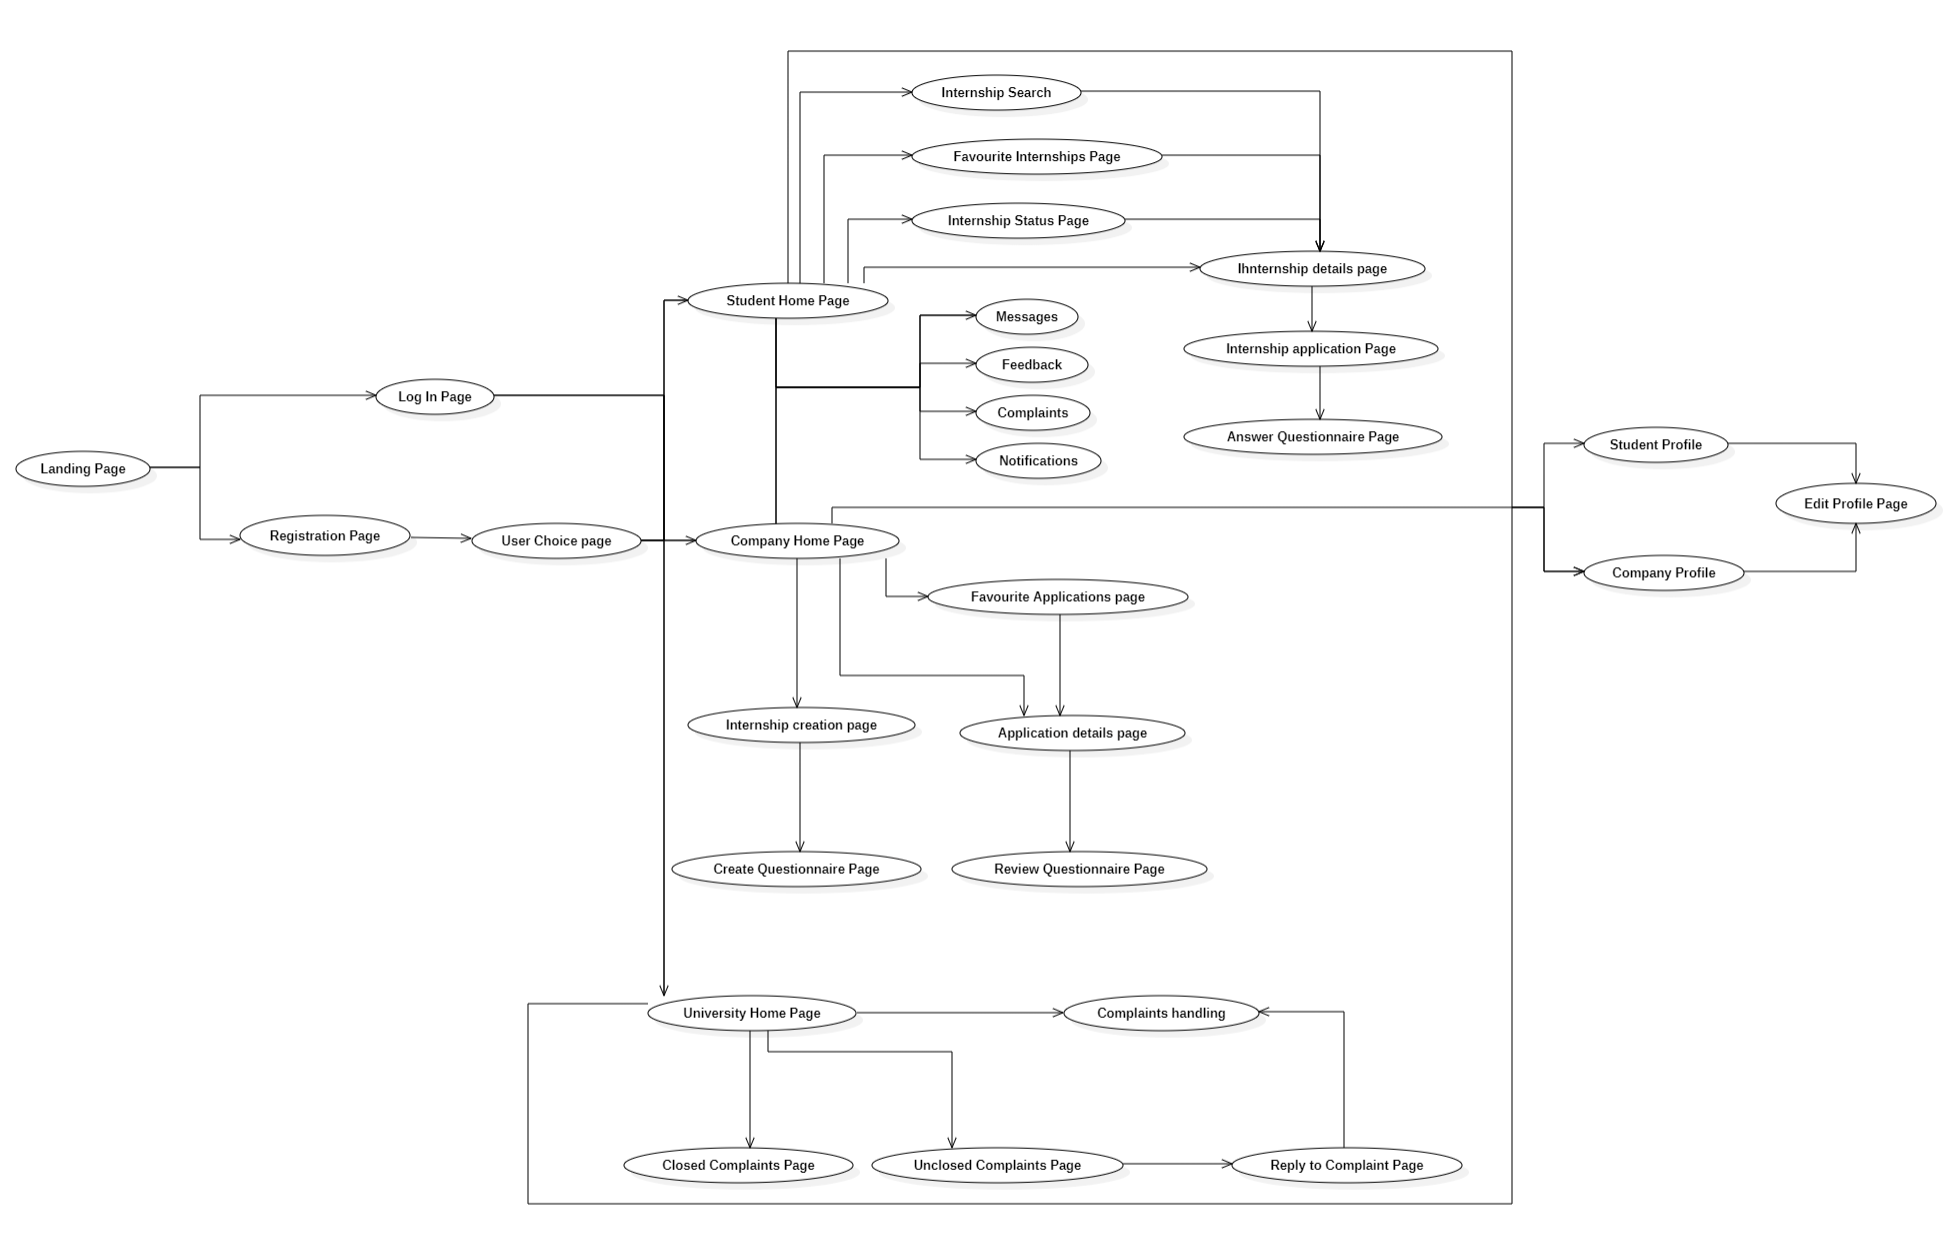
\includegraphics[width=1\linewidth]{DD/Images/Interface Images/usecasediagram.png}
    \caption{Enter Caption}
    \label{fig:enter-label}
\end{figure}

The provided graph offers a comprehensive overview of the S\&C system’s pages, illustrating their connections and navigation pathways for users. In the graph, interfaces that serve the same function for multiple users are shown only once, avoiding repetition and preventing confusion about their shared use. Communication between entities is represented separately, with arrows indicating their interactions. This approach is designed to enhance the clarity and ease of comprehension of the graph. Each page is described in the section below, providing further details on its functions and user interactions.





\section{Interfaces}

This initial illustration depicts the platform's homepage, where users can choose to log in or sign up. [Figure \ref{fig:Landing Page}]

\begin{figure}[H]
    \centering
    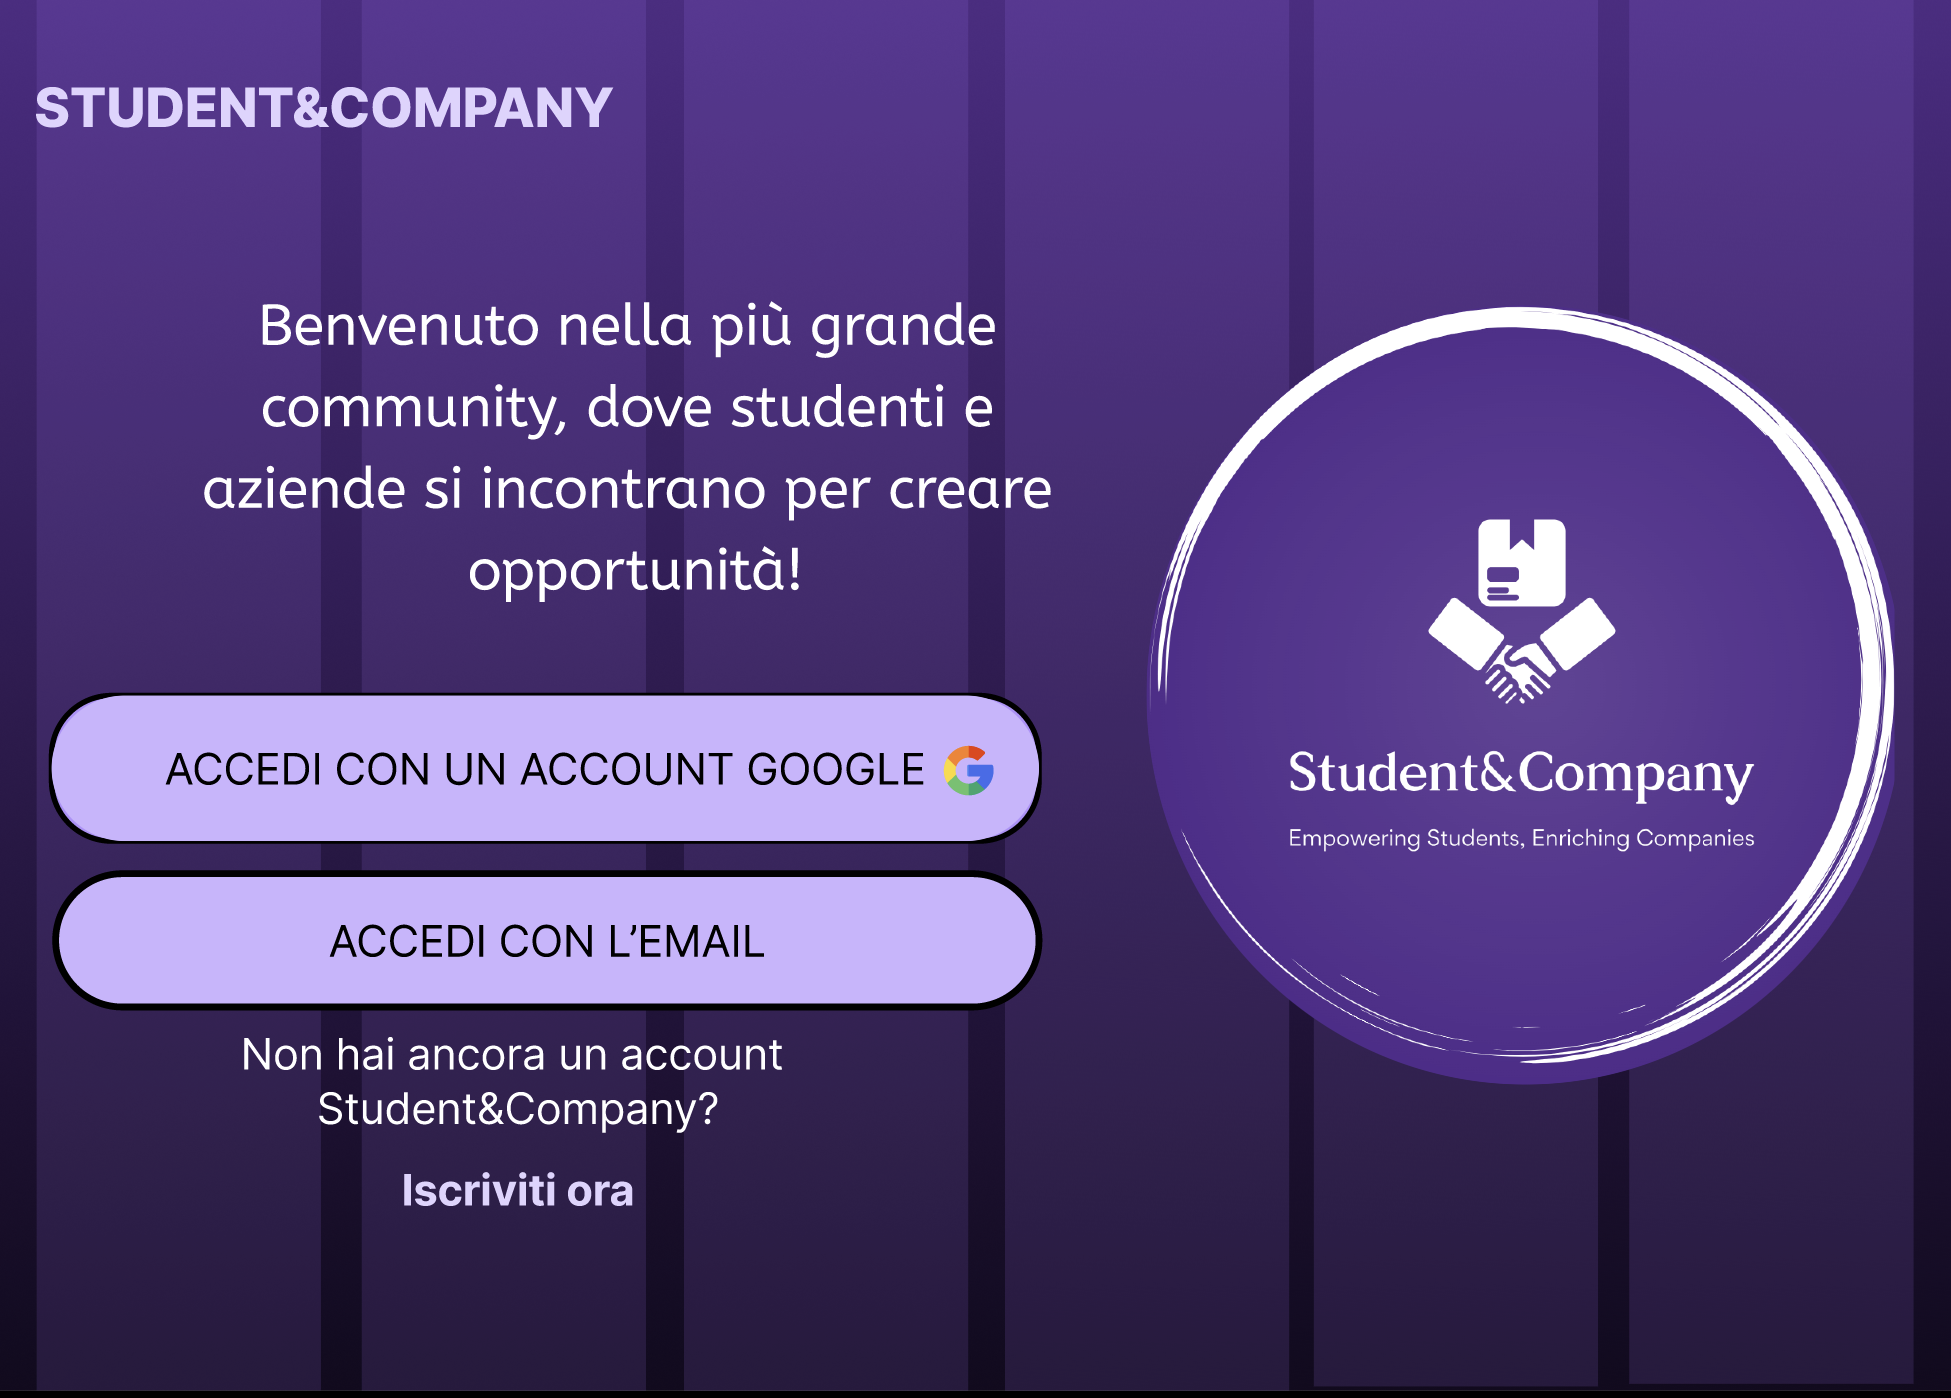
\includegraphics[width=0.5\linewidth]{Images/Interface Images//log in sing up/image.png}
    \caption{Landing Page}
    \label{fig:Landing Page}
\end{figure}

After a user decides to create an account, they will be asked their role as either a student, company or a university. [Figure \ref{fig:Choice page}] 

\begin{figure} [H]
    \centering
    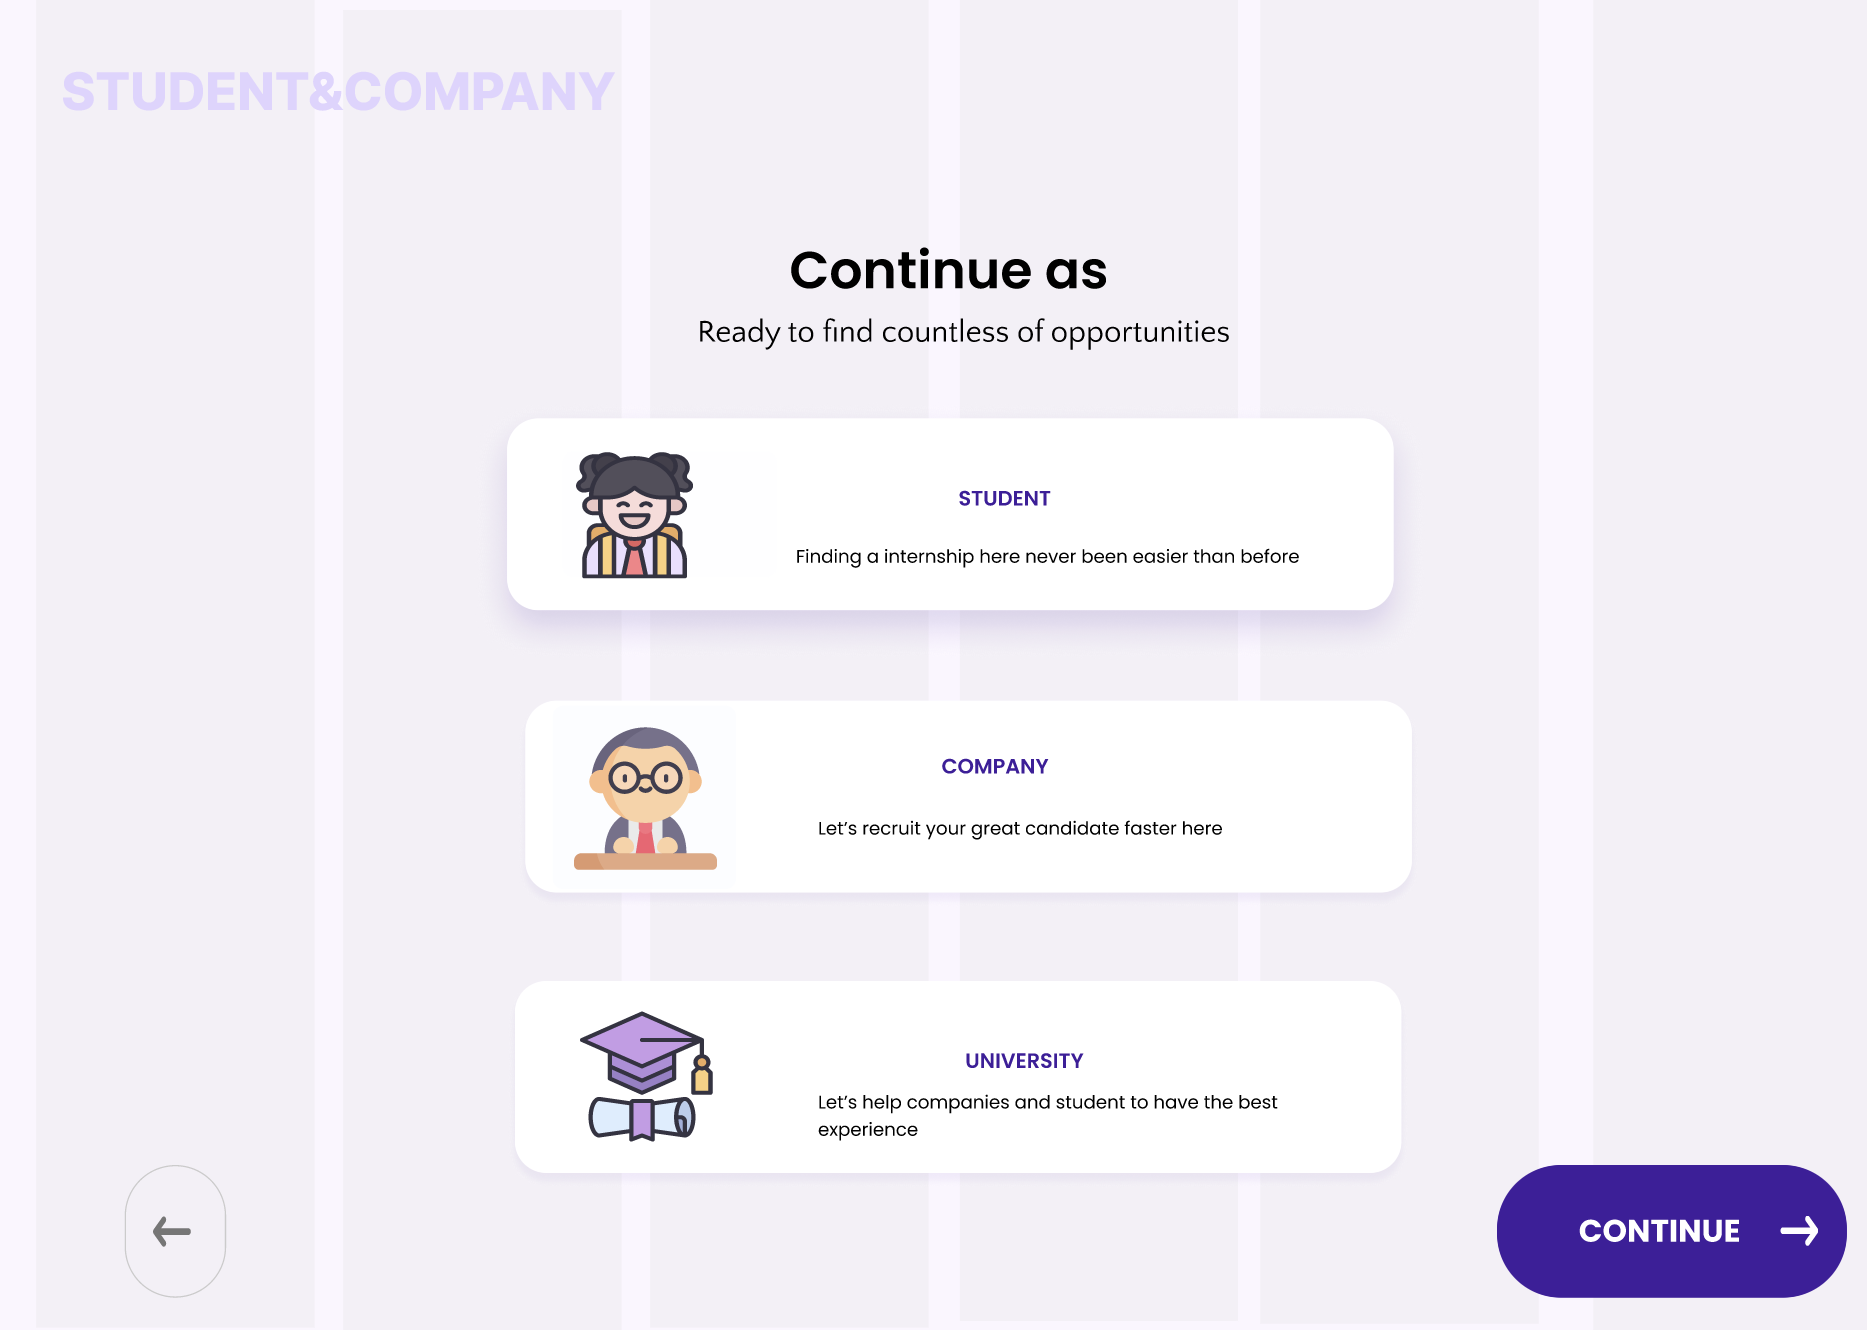
\includegraphics[width=0.5\linewidth]{Images/Interface Images/log in sing up/Screenshot 2024-12-03 110046.png}
    \caption{Choice page}
    \label{fig:Choice page}
\end{figure}

Depending on the role decided by the user, they will be prompted to input various information that can vary based on the specific role. [Figures \ref{fig:Create account for Students}, \ref{fig: Create account for companies}, \ref{fig:Create account for Universities}] 

\begin{figure} [H]
    \centering
    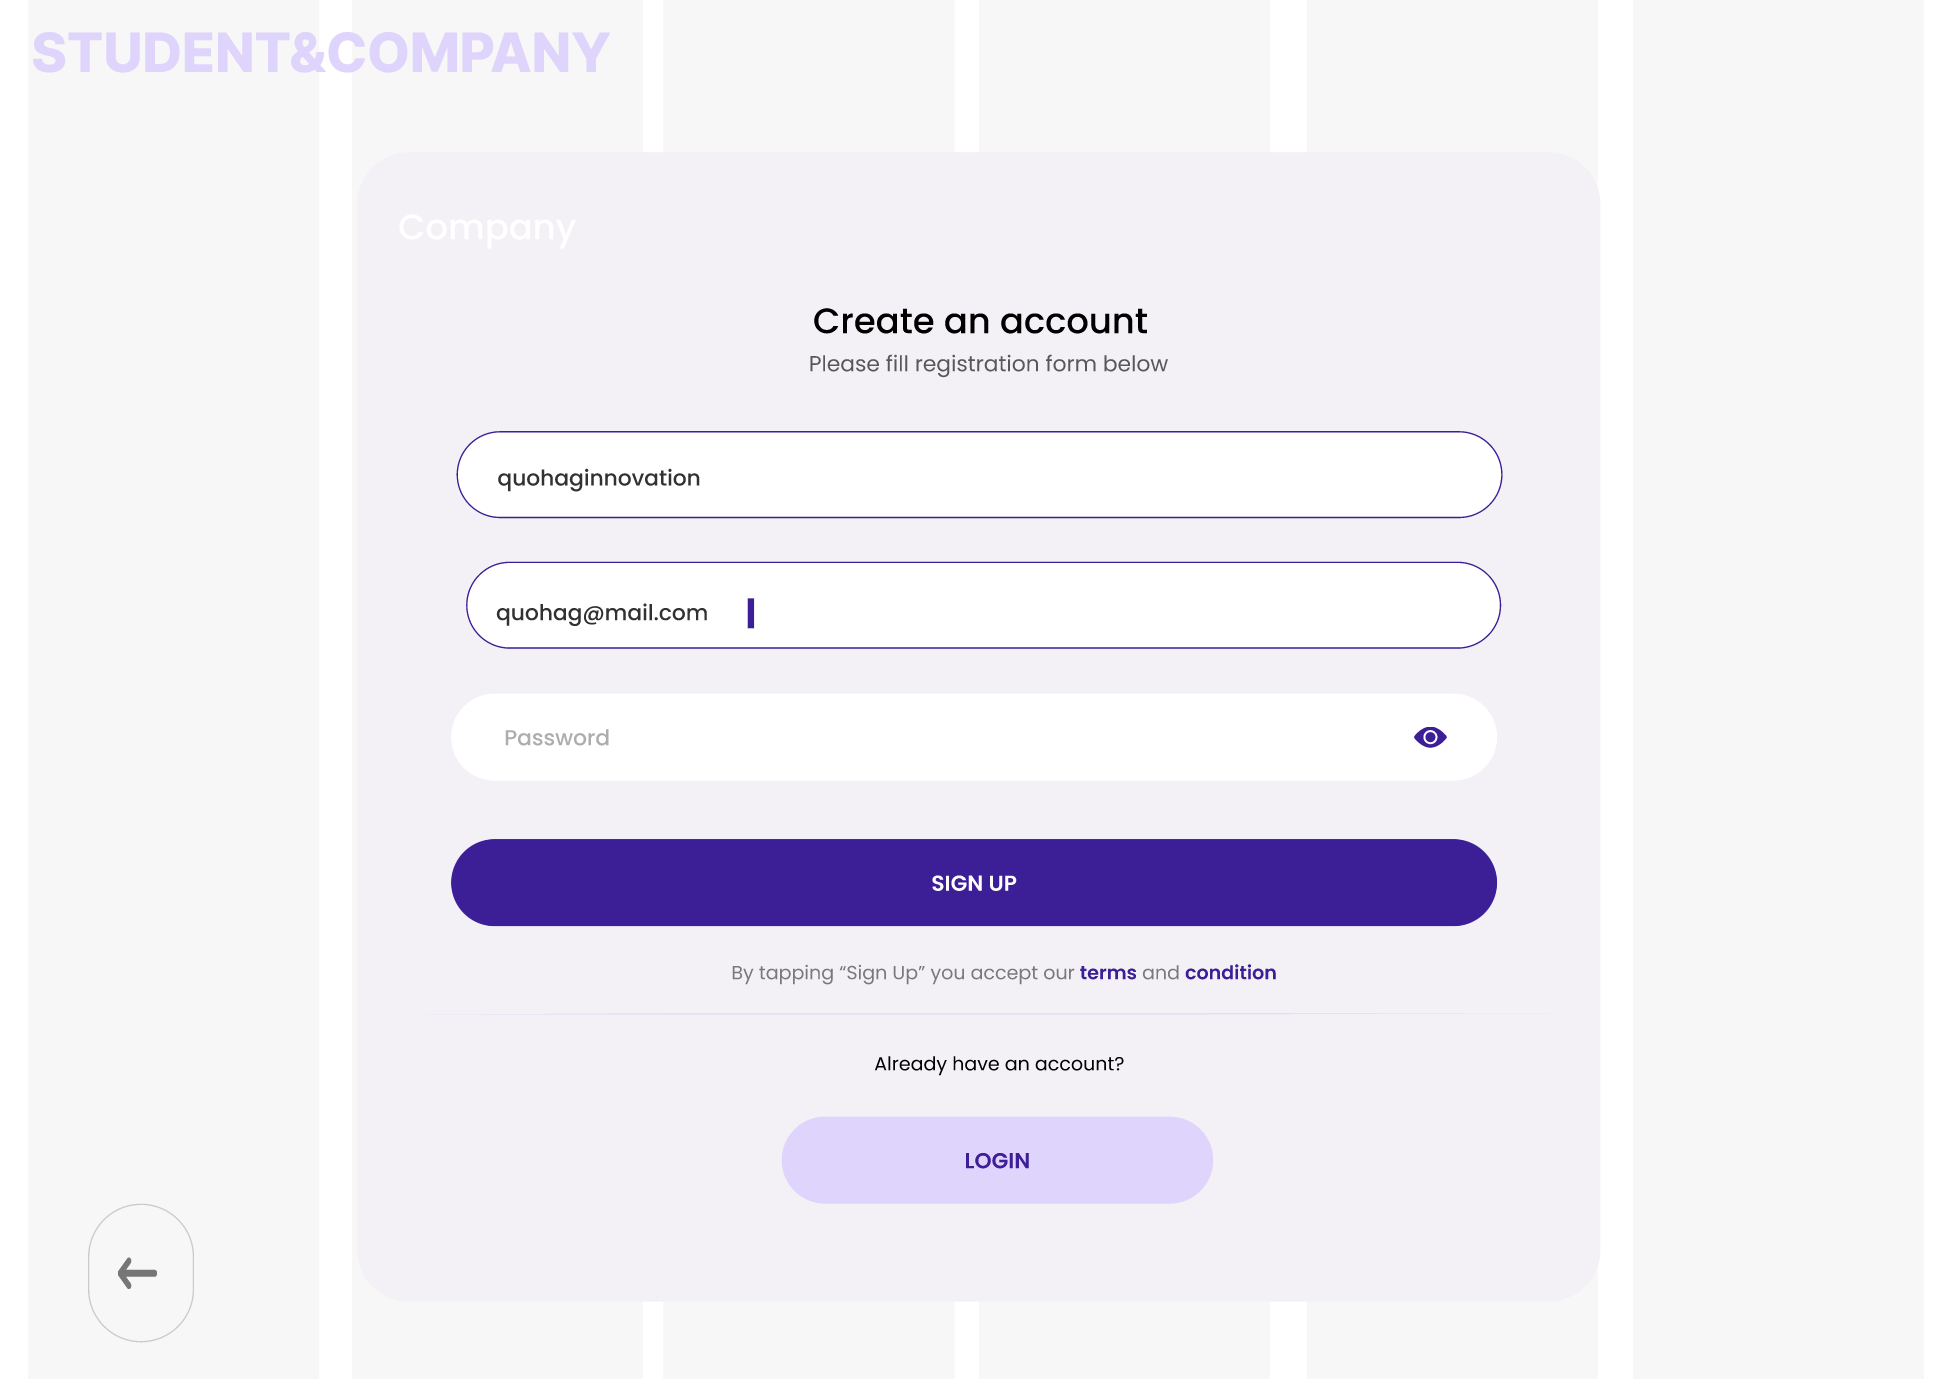
\includegraphics[width=0.5\linewidth]{Images/Interface Images/log in sing up/Screenshot 2024-12-12 045014.png}
    \caption{Create account for Companies }
    \label{fig: Create account for companies}
\end{figure}

\begin{figure} [H]
    \centering
    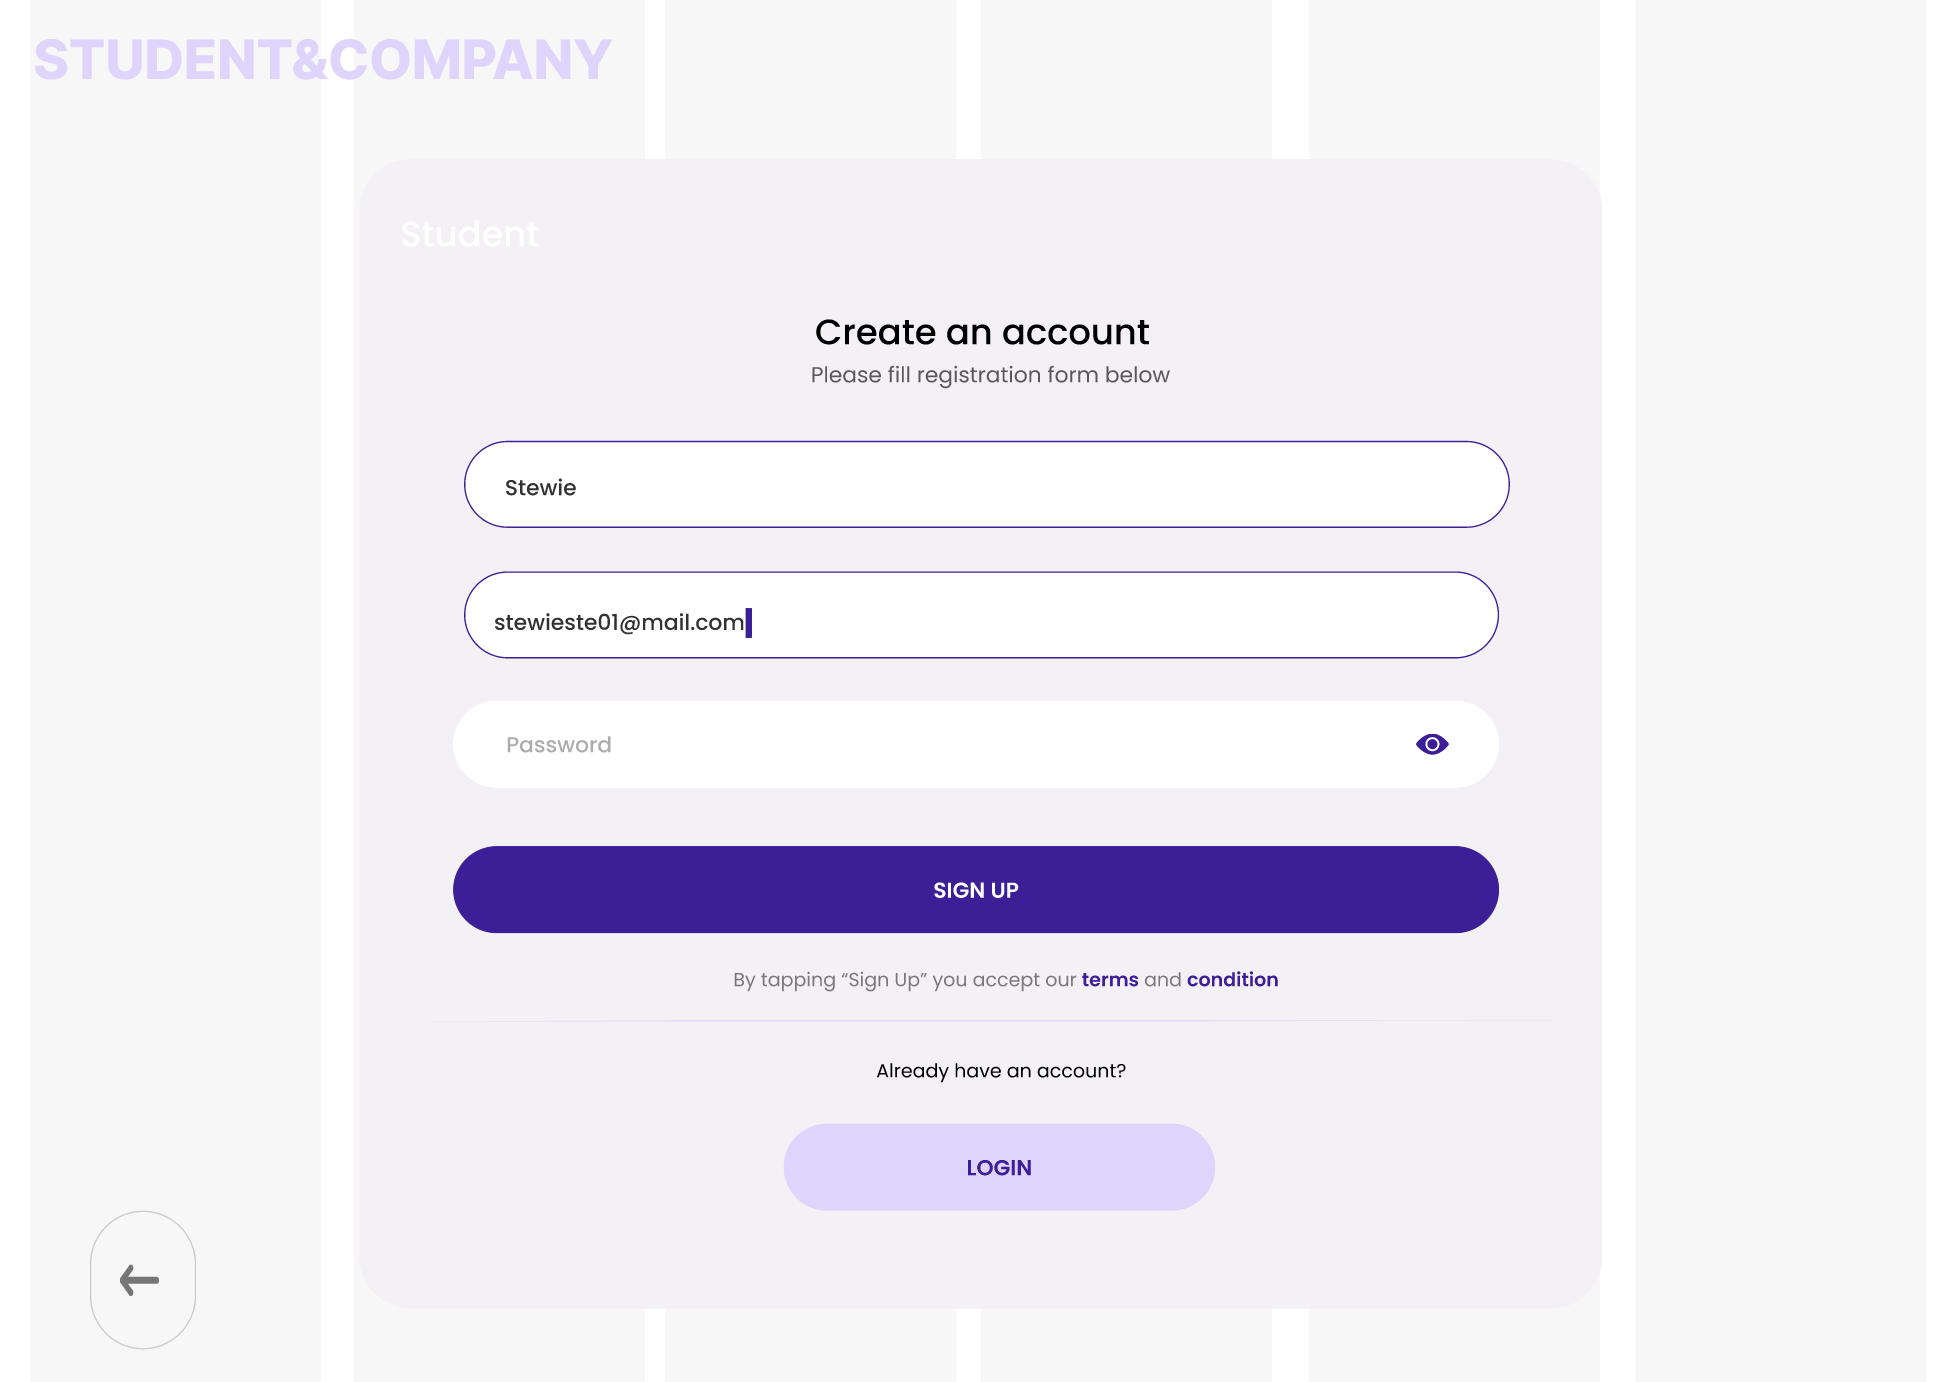
\includegraphics[width=0.5\linewidth]{Images/Interface Images/log in sing up/Screenshot 2024-12-12 045029.png}
    \caption{Create account for Students}
    \label{fig:Create account for Students}
\end{figure}

\begin{figure} [H]
    \centering
    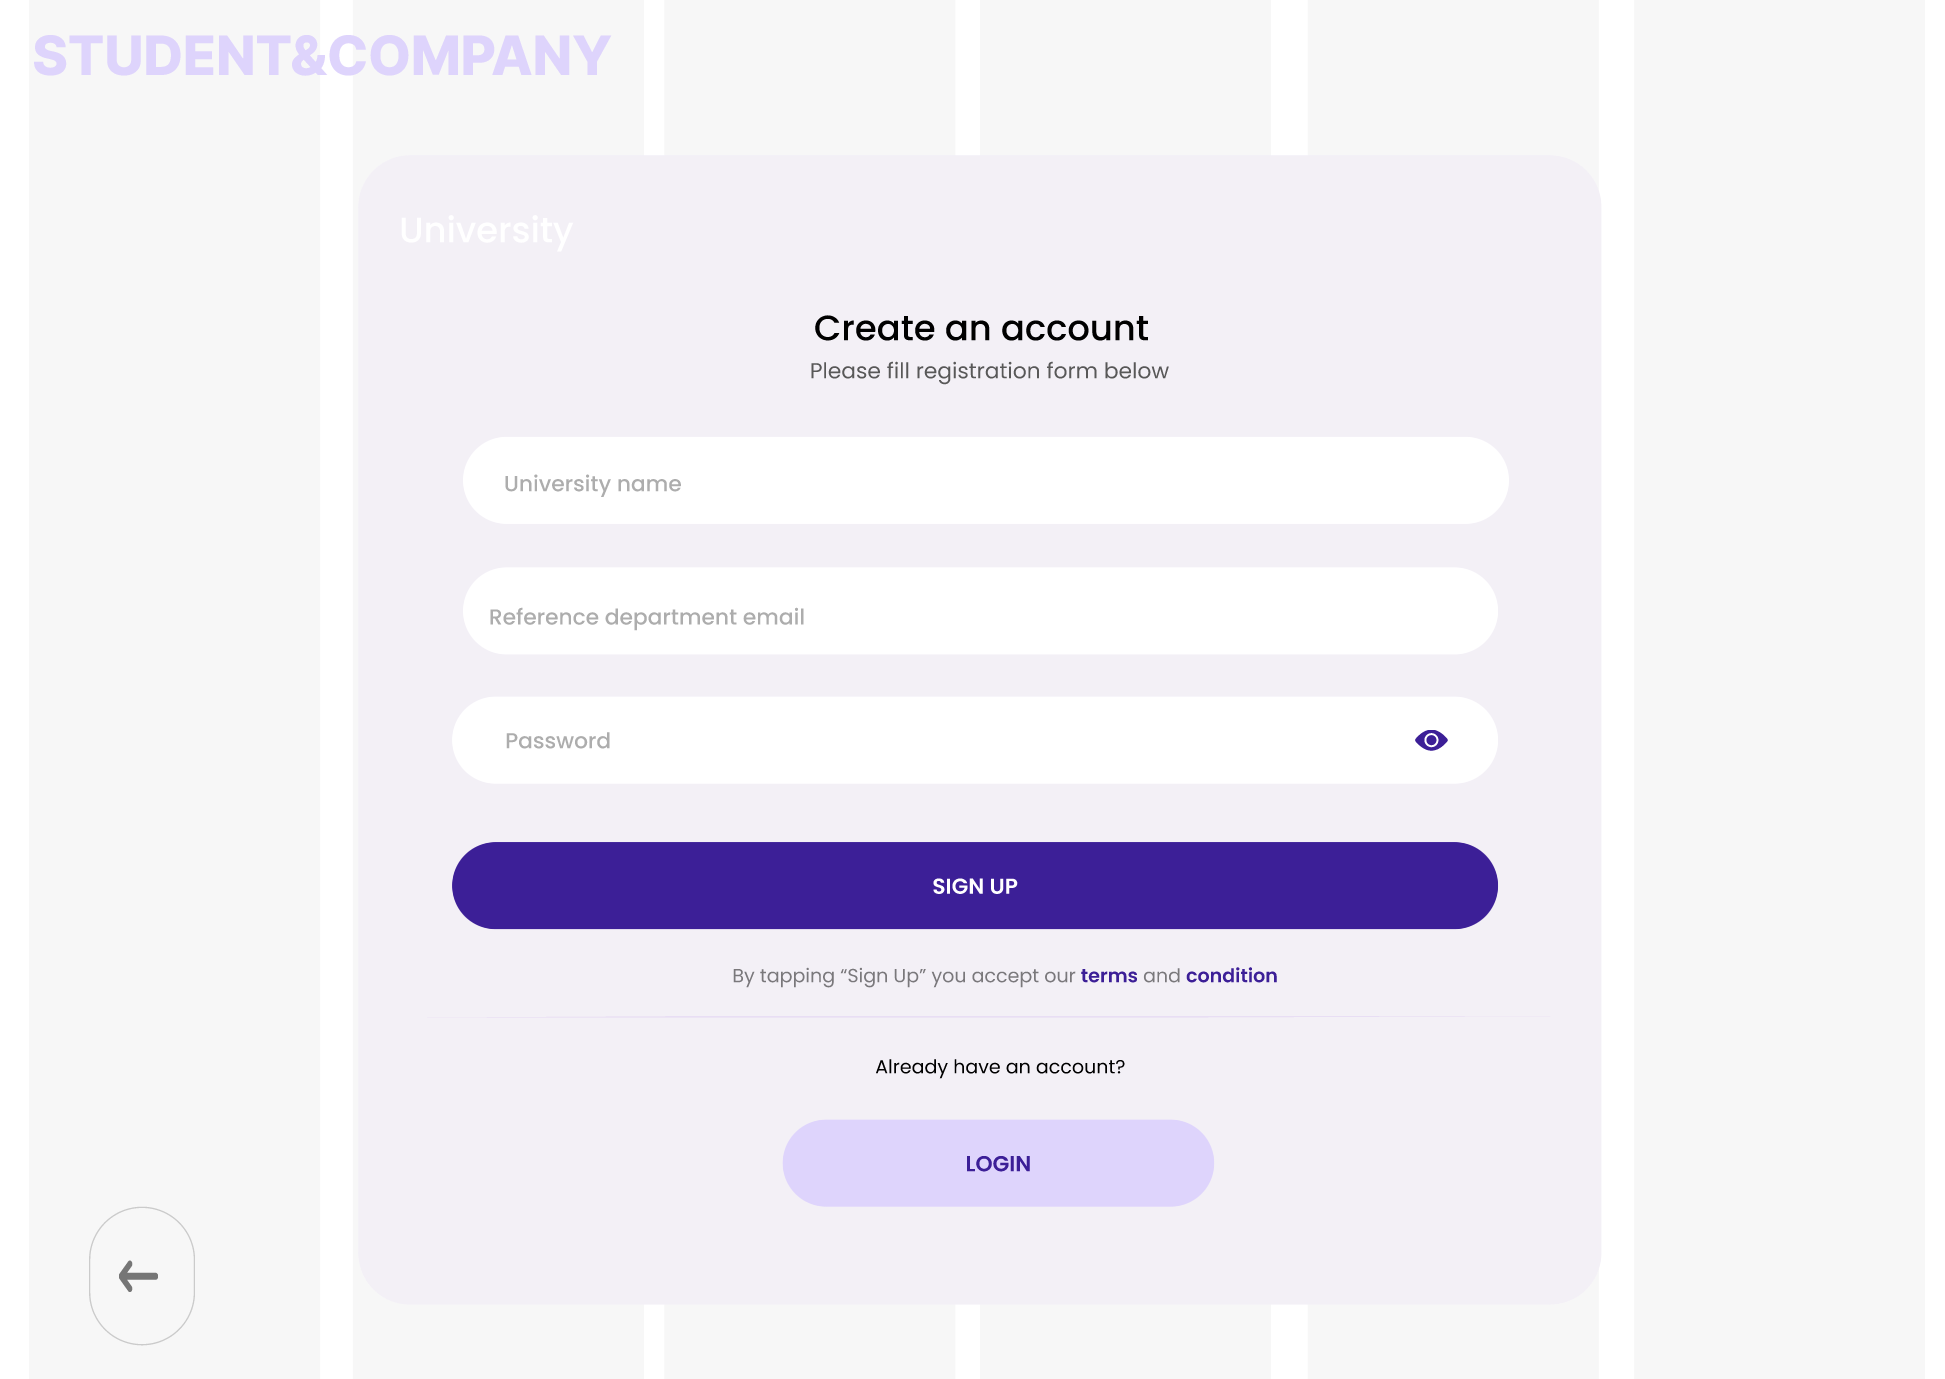
\includegraphics[width=0.5\linewidth]{Images/Interface Images/log in sing up/Screenshot 2024-12-12 045042.png}
    \caption{Create account for Universities}
    \label{fig:Create account for Universities}
\end{figure}

Users with an existing account can access the platform by clicking the appropriate button on the homepage, which directs them to the login page. From there, they can log in using their username and password or by signing in with their Google or Facebook account. If a user mistakenly selects the login option without having an account, they can simply click the "Create Account" button to navigate to the registration page. [Figures \ref{fig:Company Sign in}, \ref{fig: Student Sign in}, \ref{fig:University Sign in}]

\begin{figure} [H]
    \centering
    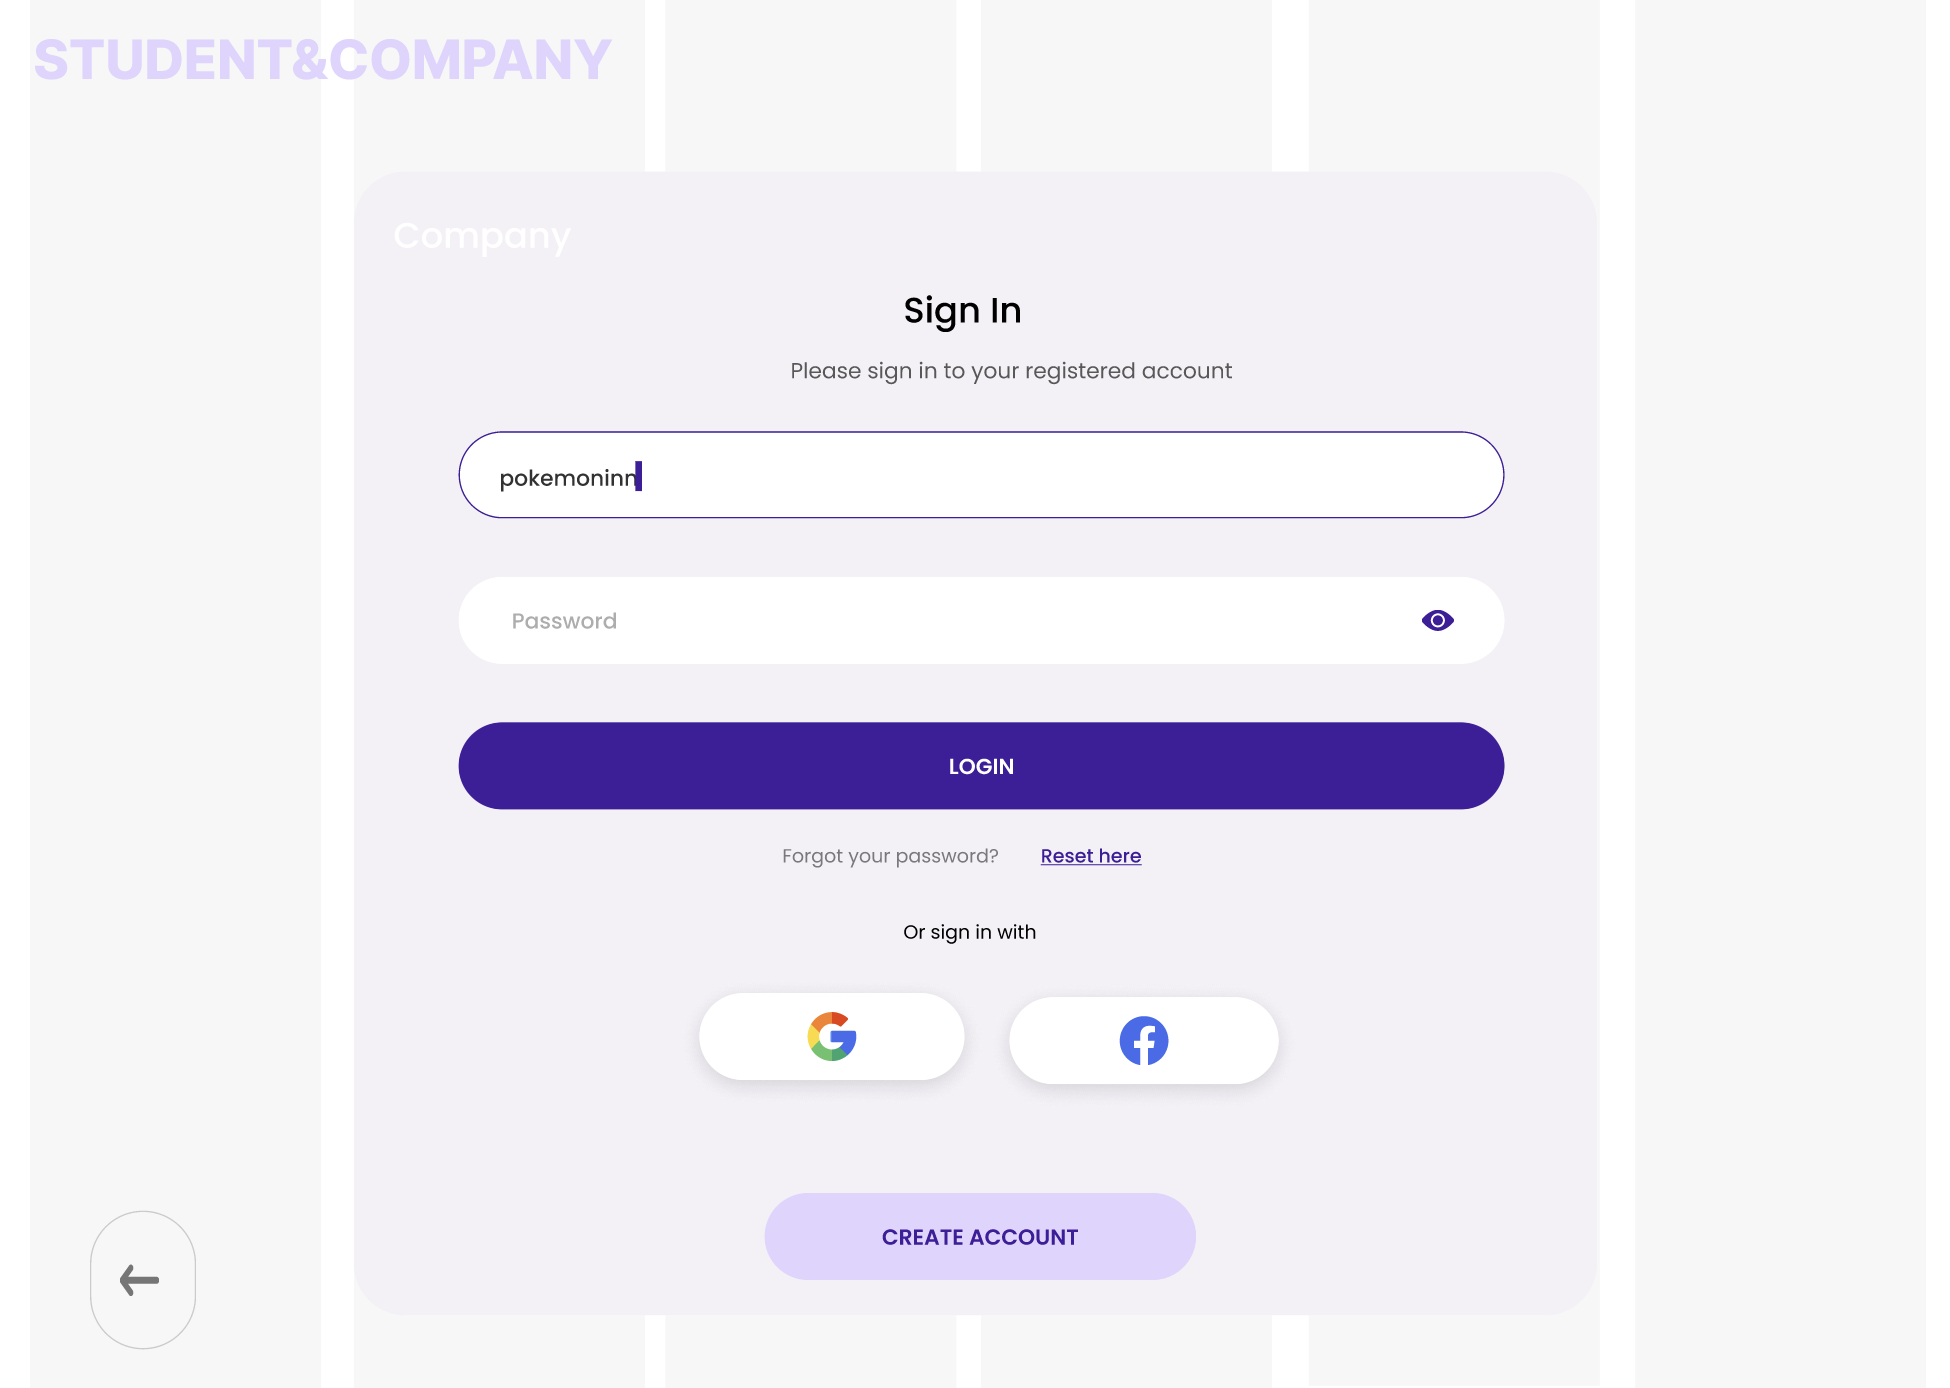
\includegraphics[width=0.5\linewidth]{Images/Interface Images/log in sing up/Screenshot 2024-12-12 045111.png}
    \caption{Company Sign in}
    \label{fig:Company Sign in}
\end{figure}

\begin{figure} [H]
    \centering
    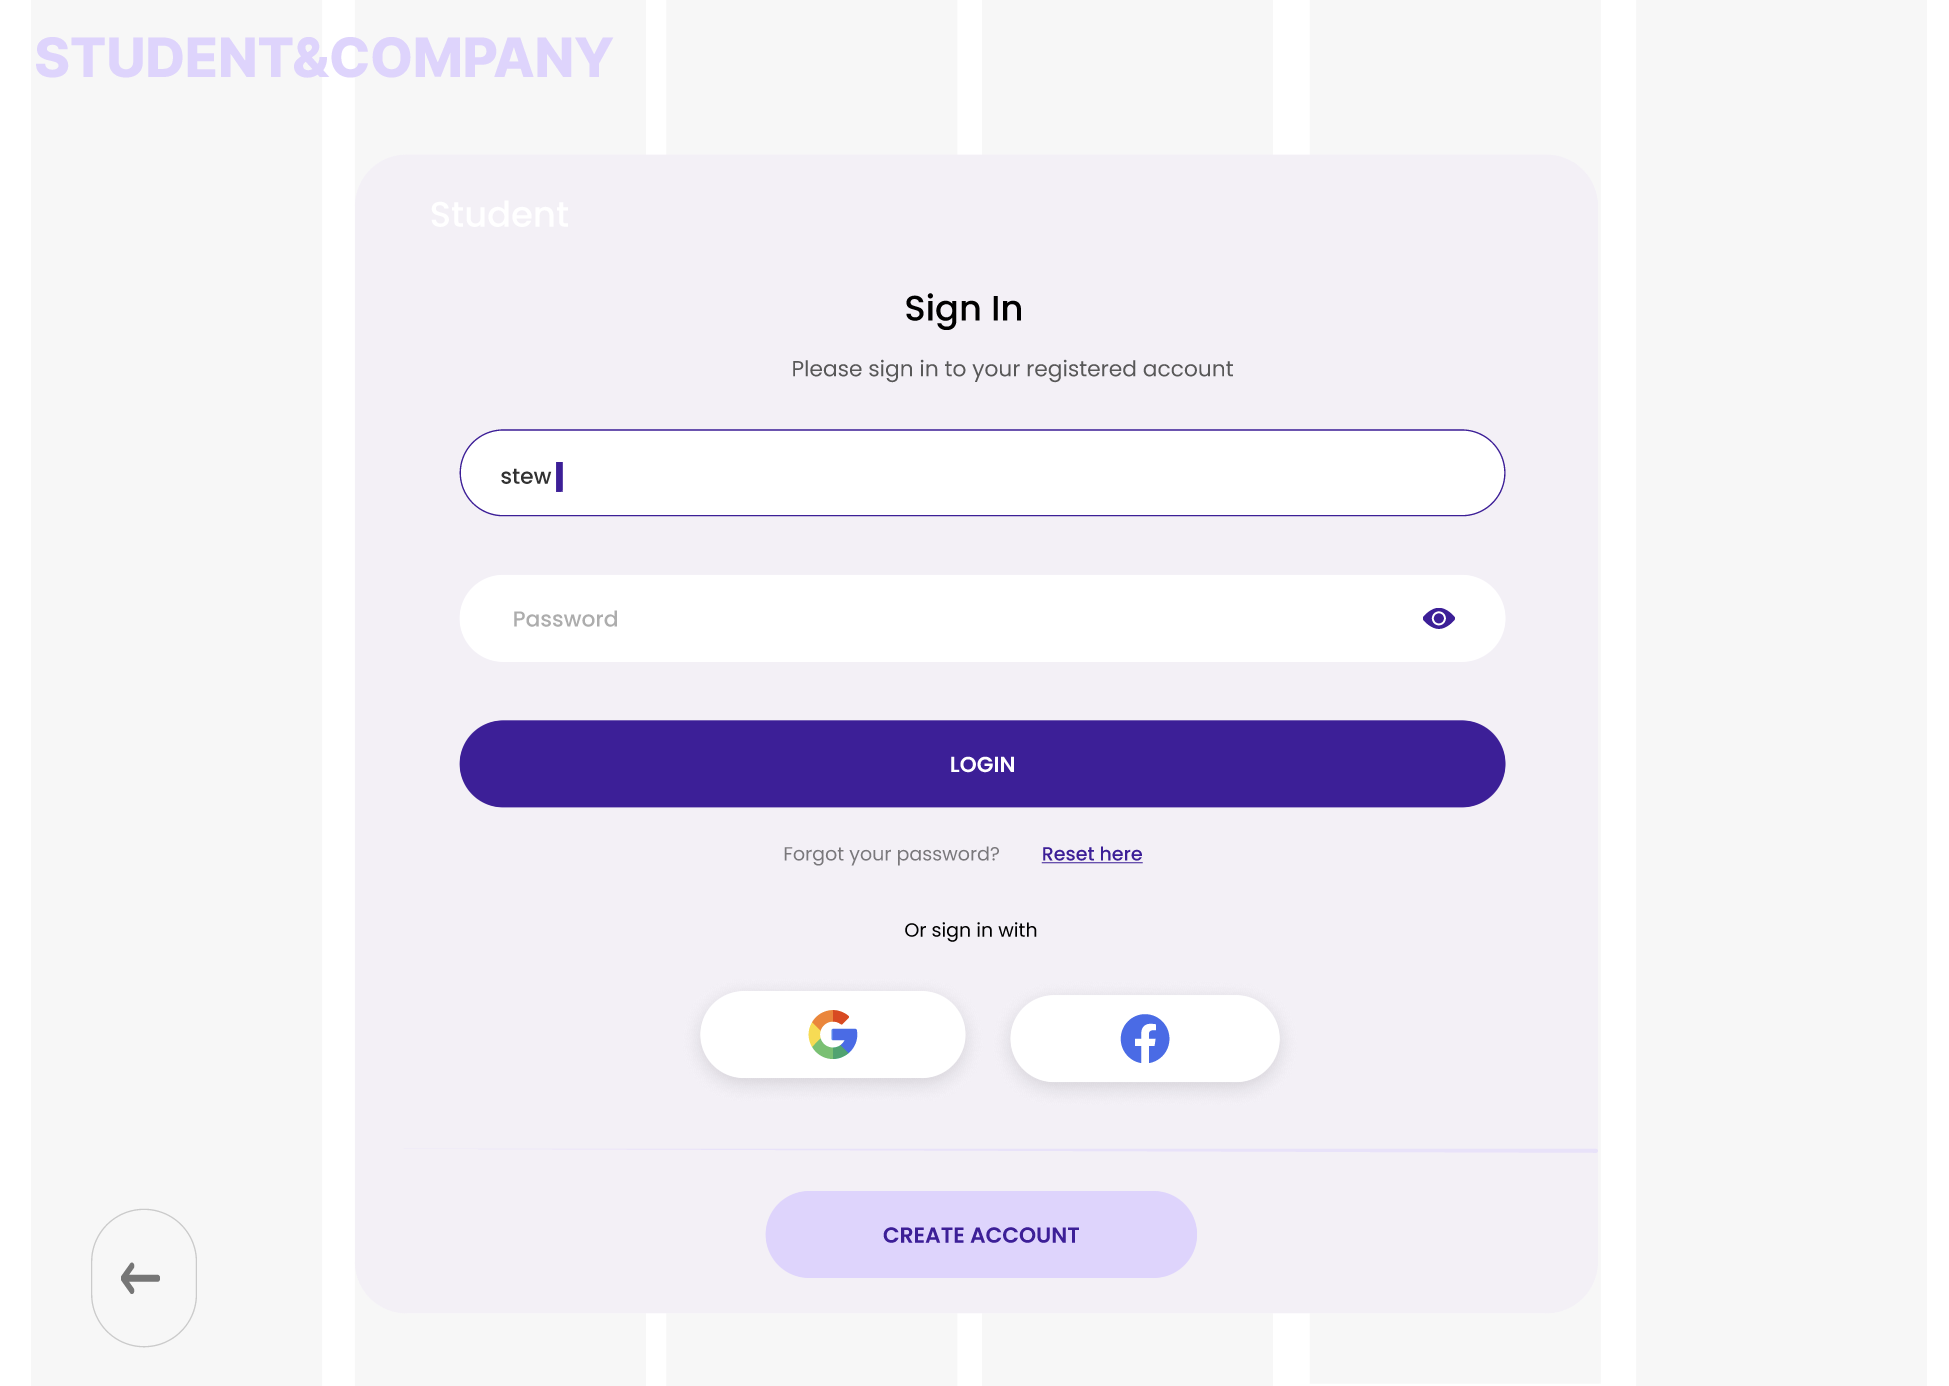
\includegraphics[width=0.5\linewidth]{Images/Interface Images/log in sing up/Screenshot 2024-12-12 045127.png}
    \caption{Student Sign in}
    \label{fig: Student Sign in}
\end{figure}

\begin{figure} [H]
    \centering
    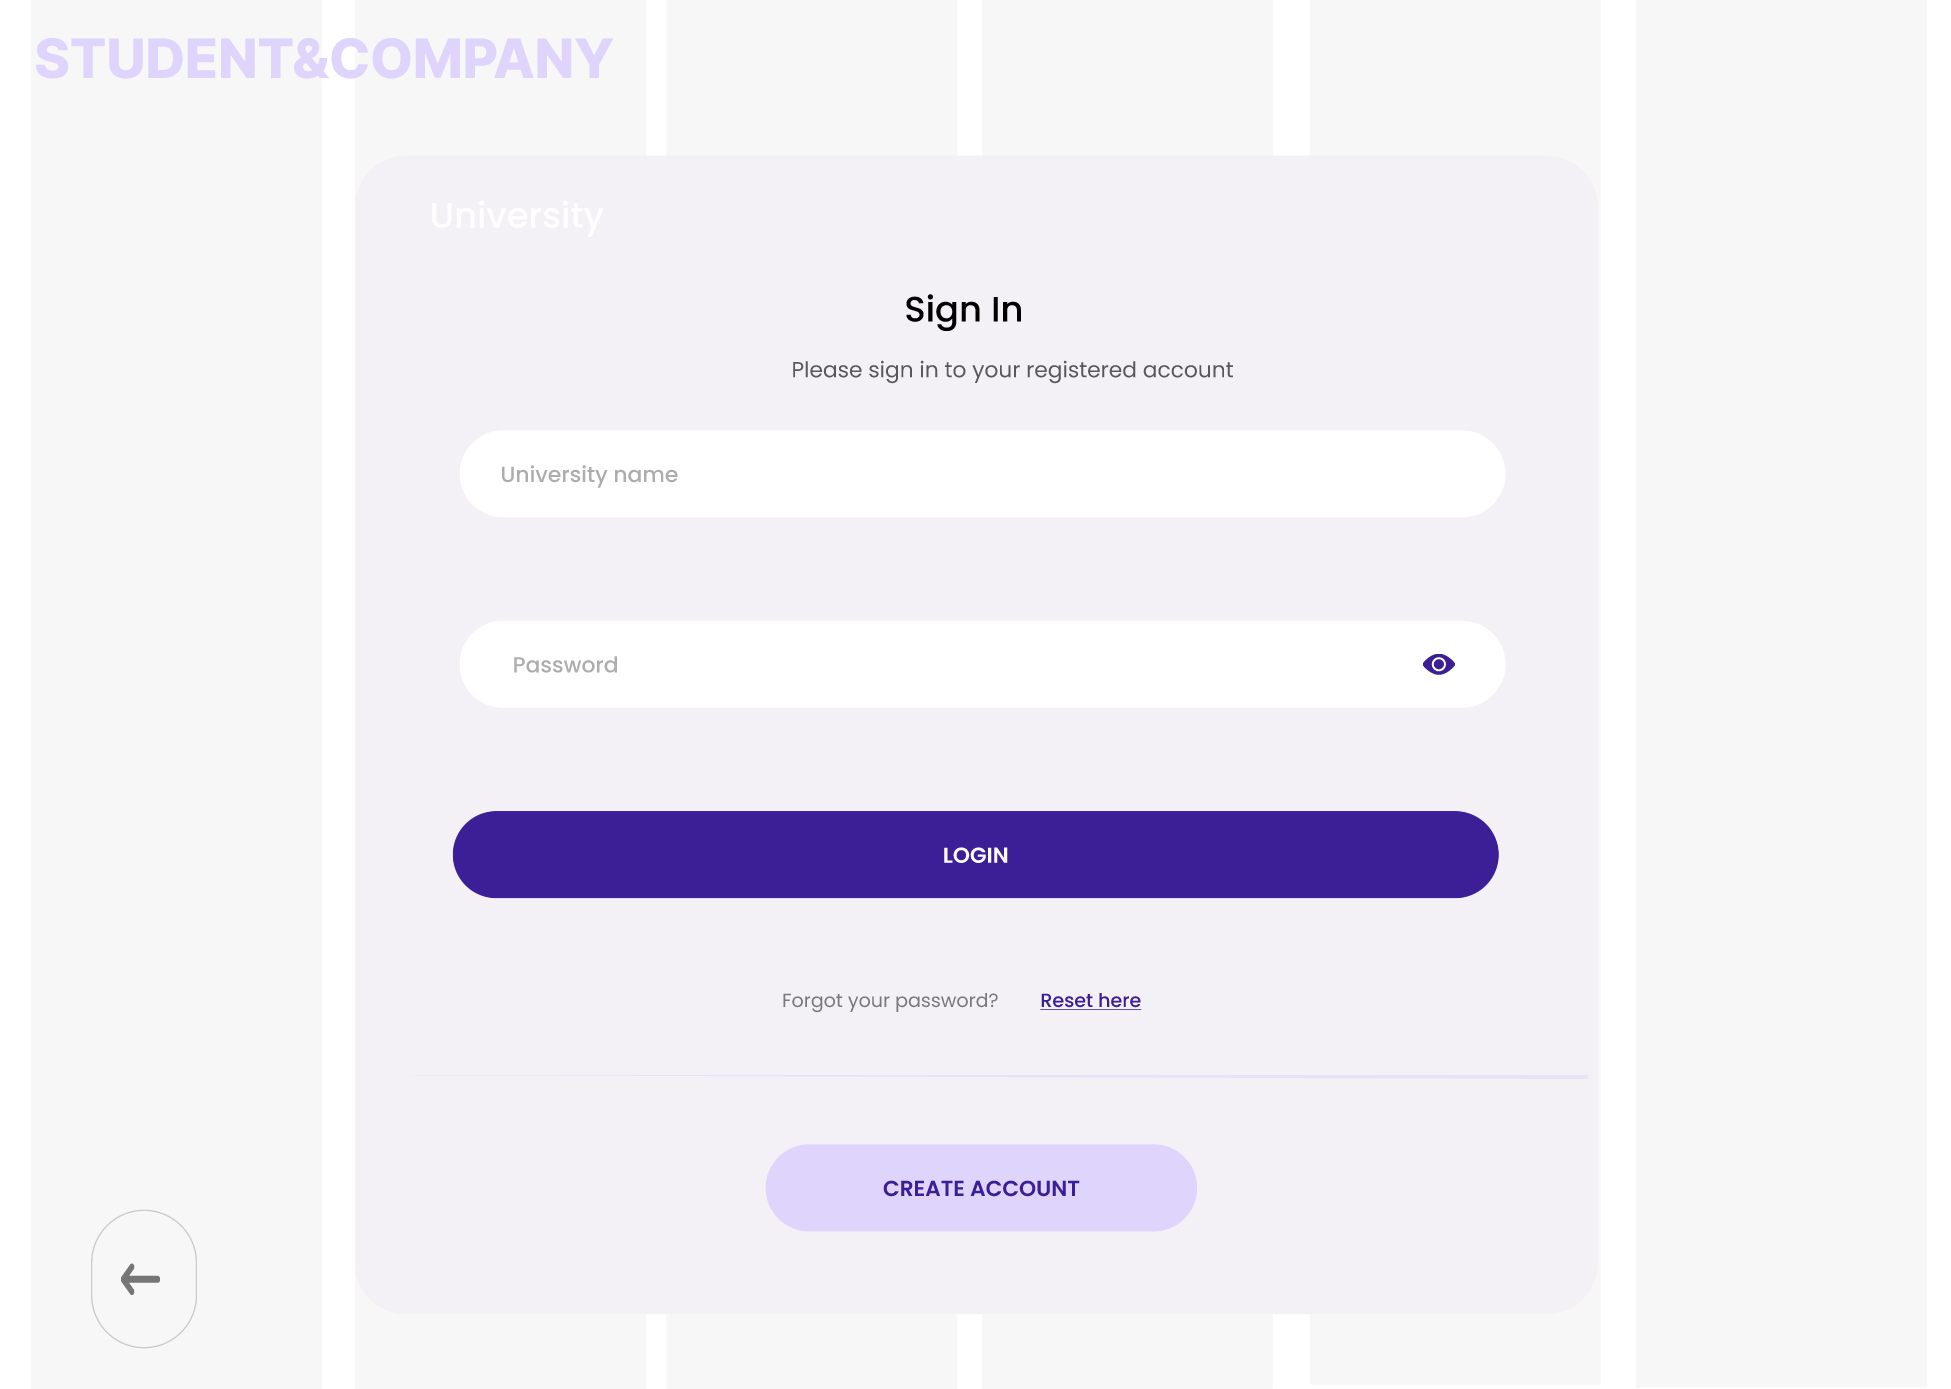
\includegraphics[width=0.5\linewidth]{RASD/Interface Images/log in sing up/Screenshot 2024-12-12 045139.png}
    \caption{University Sign in}
    \label{fig:University Sign in}
\end{figure}


\subsection{Company Interfaces}

The company's Dashboard [Figure \ref{fig:Company Home page}] serves as the central hub for all platform operations. From this main page, the company can easily access essential information, including its profile, notifications, proposed internships, and applications submitted by students. Additionally, it allows the company to communicate with students after the internship application process, as well as provide feedback or submit complaints.

\begin{figure} [H]
    \centering
    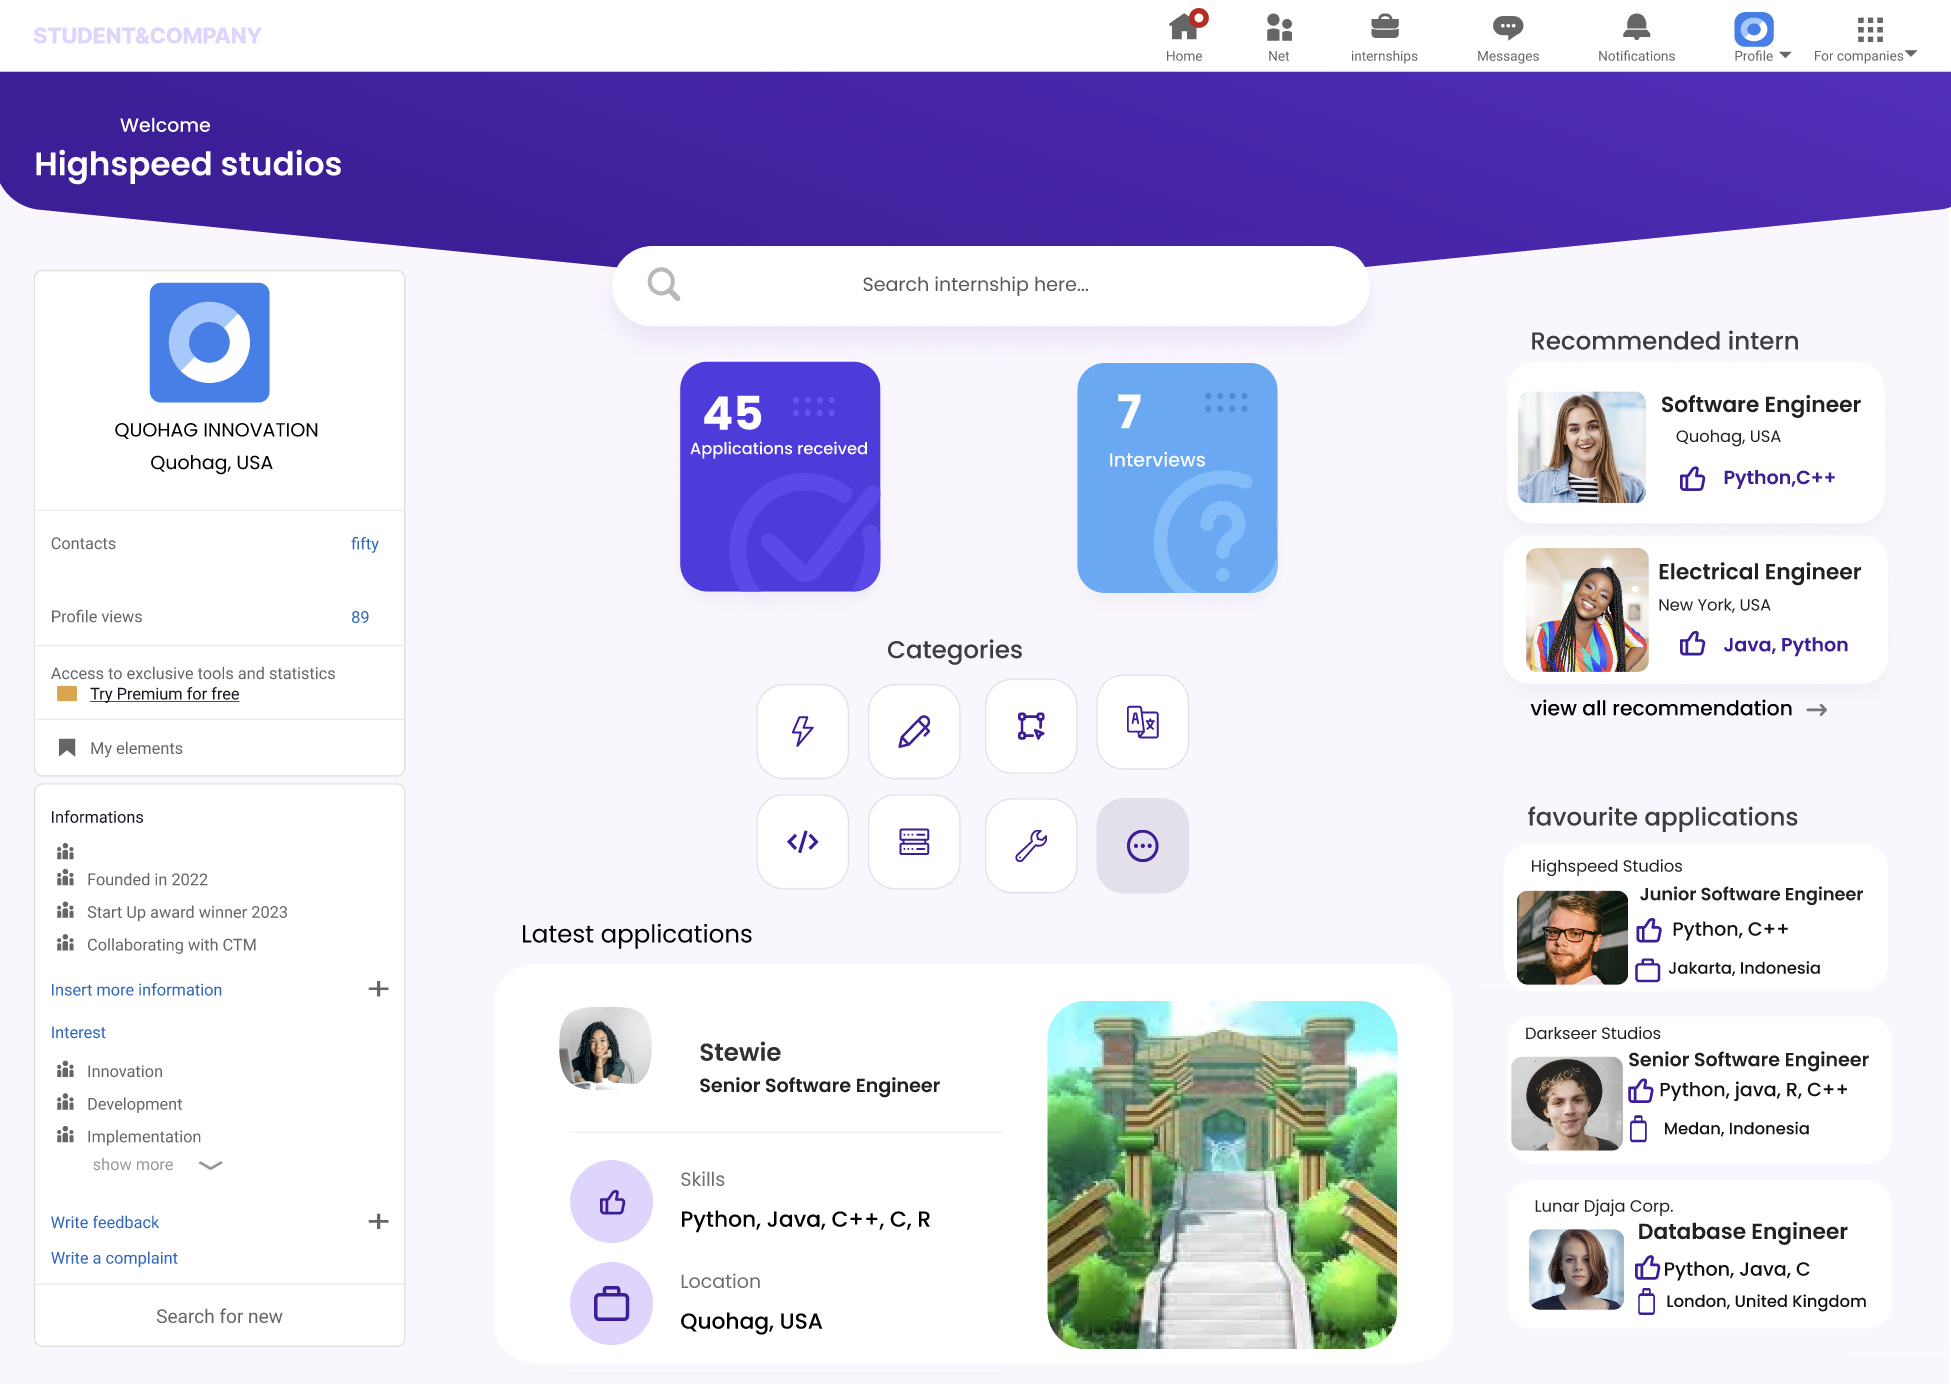
\includegraphics[width=0.5\linewidth]{Images/Interface Images/company interface/Screenshot 2024-12-12 045319.png}
    \caption{Company Home page}
    \label{fig:Company Home page}
\end{figure}

Below, we can see the structure of a company's personal profile. It includes key details such as location, field of activity, objectives, and a dedicated section for managing internships. To edit the profile, the company simply clicks on the desired section and follows the platform's guidance. Additionally, the platform offers suggestions to enhance the provided information, making it more appealing to potential viewers[ Figures \ref{fig:Company Personal profile}, \ref{fig:Company - Managing account}].


\begin{figure} [H]
    \centering
    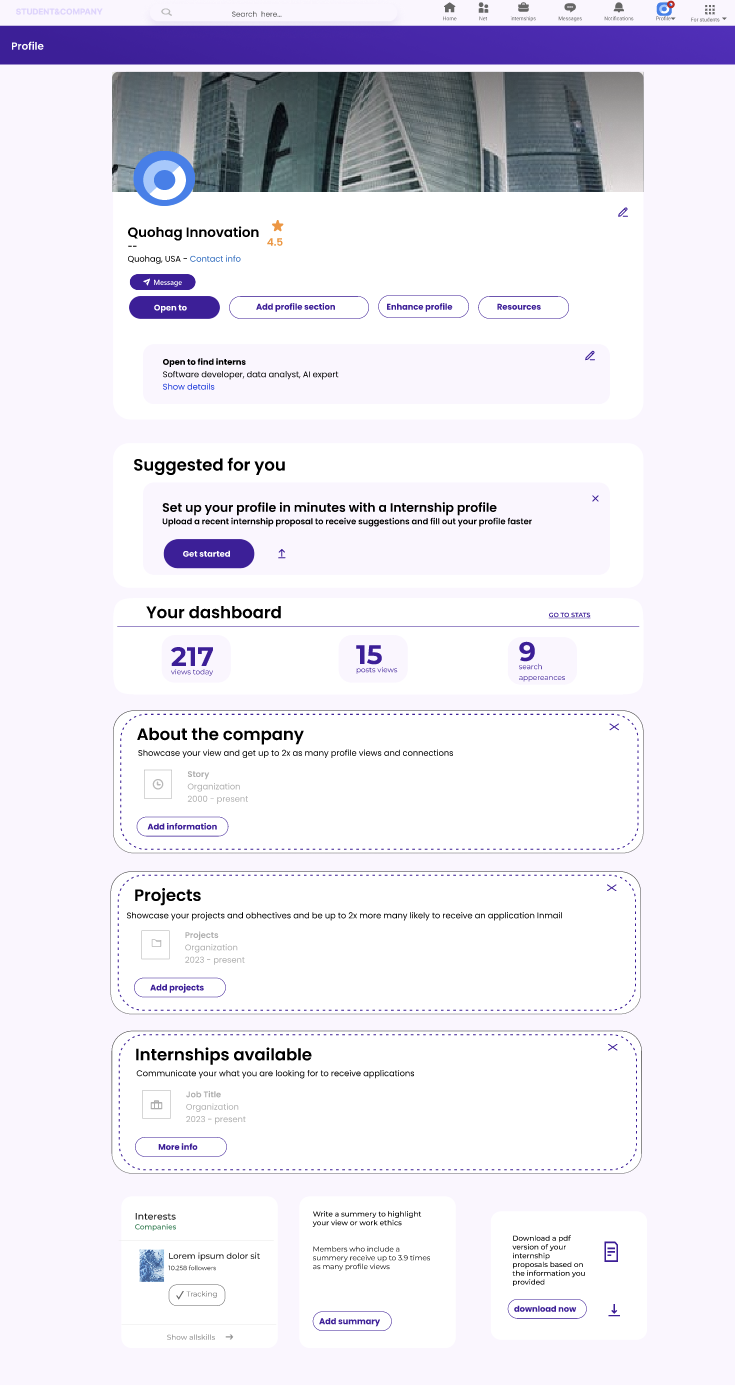
\includegraphics[width=0.5\linewidth]{Images/Interface Images/company interface/Screenshot 2024-12-12 045502.png}
    \caption{Company Personal profile}
    \label{fig:Company Personal profile}
\end{figure}

\begin{figure} [H]
    \centering
    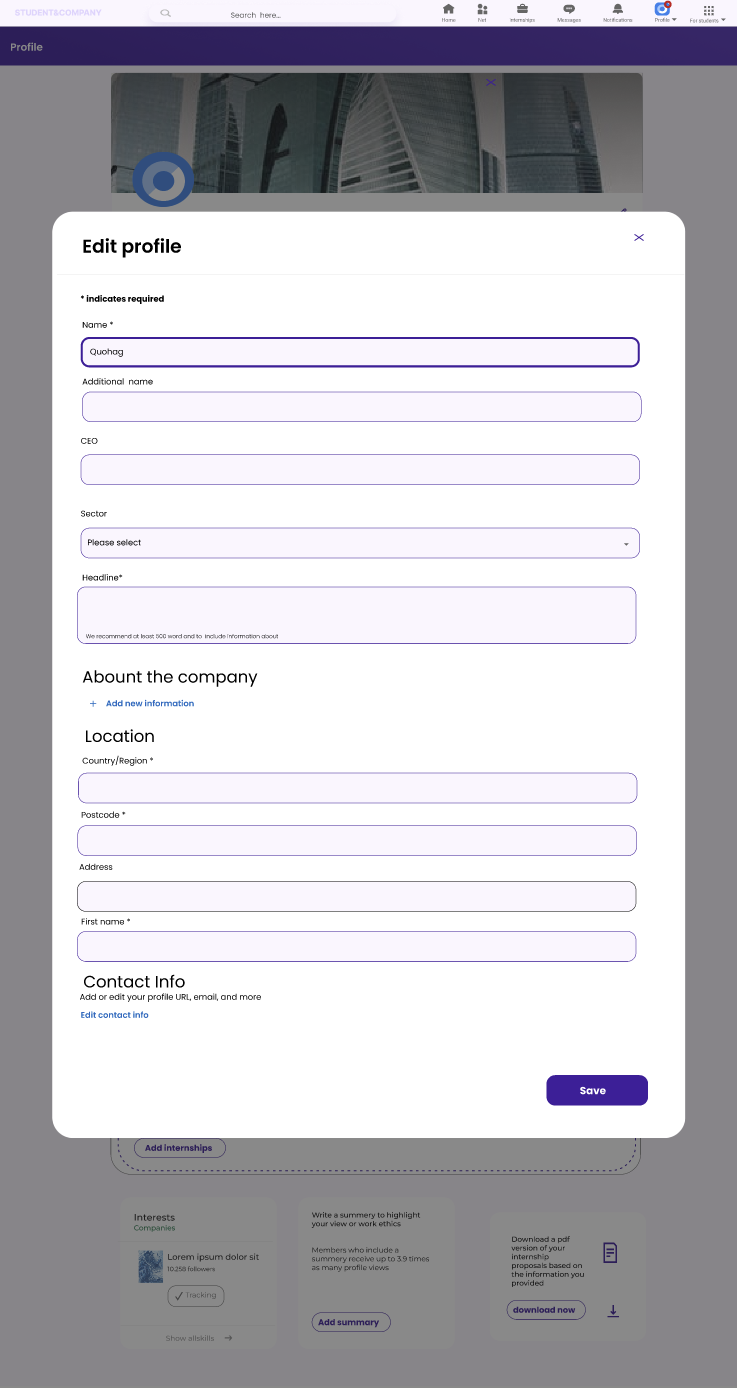
\includegraphics[width=0.5\linewidth]{Images/Interface Images/company interface/Screenshot 2024-12-12 045535.png}
    \caption{Company - Managing account}
    \label{fig:Company - Managing account}
\end{figure}


To edit internship information, the company can click on the designated button within its personal profile. From there, it can manage the internship details while also benefiting from suggestion.s provided by the platform [Figure \ref{fig:Internships management}]. 

\begin{figure} [H]
    \centering
    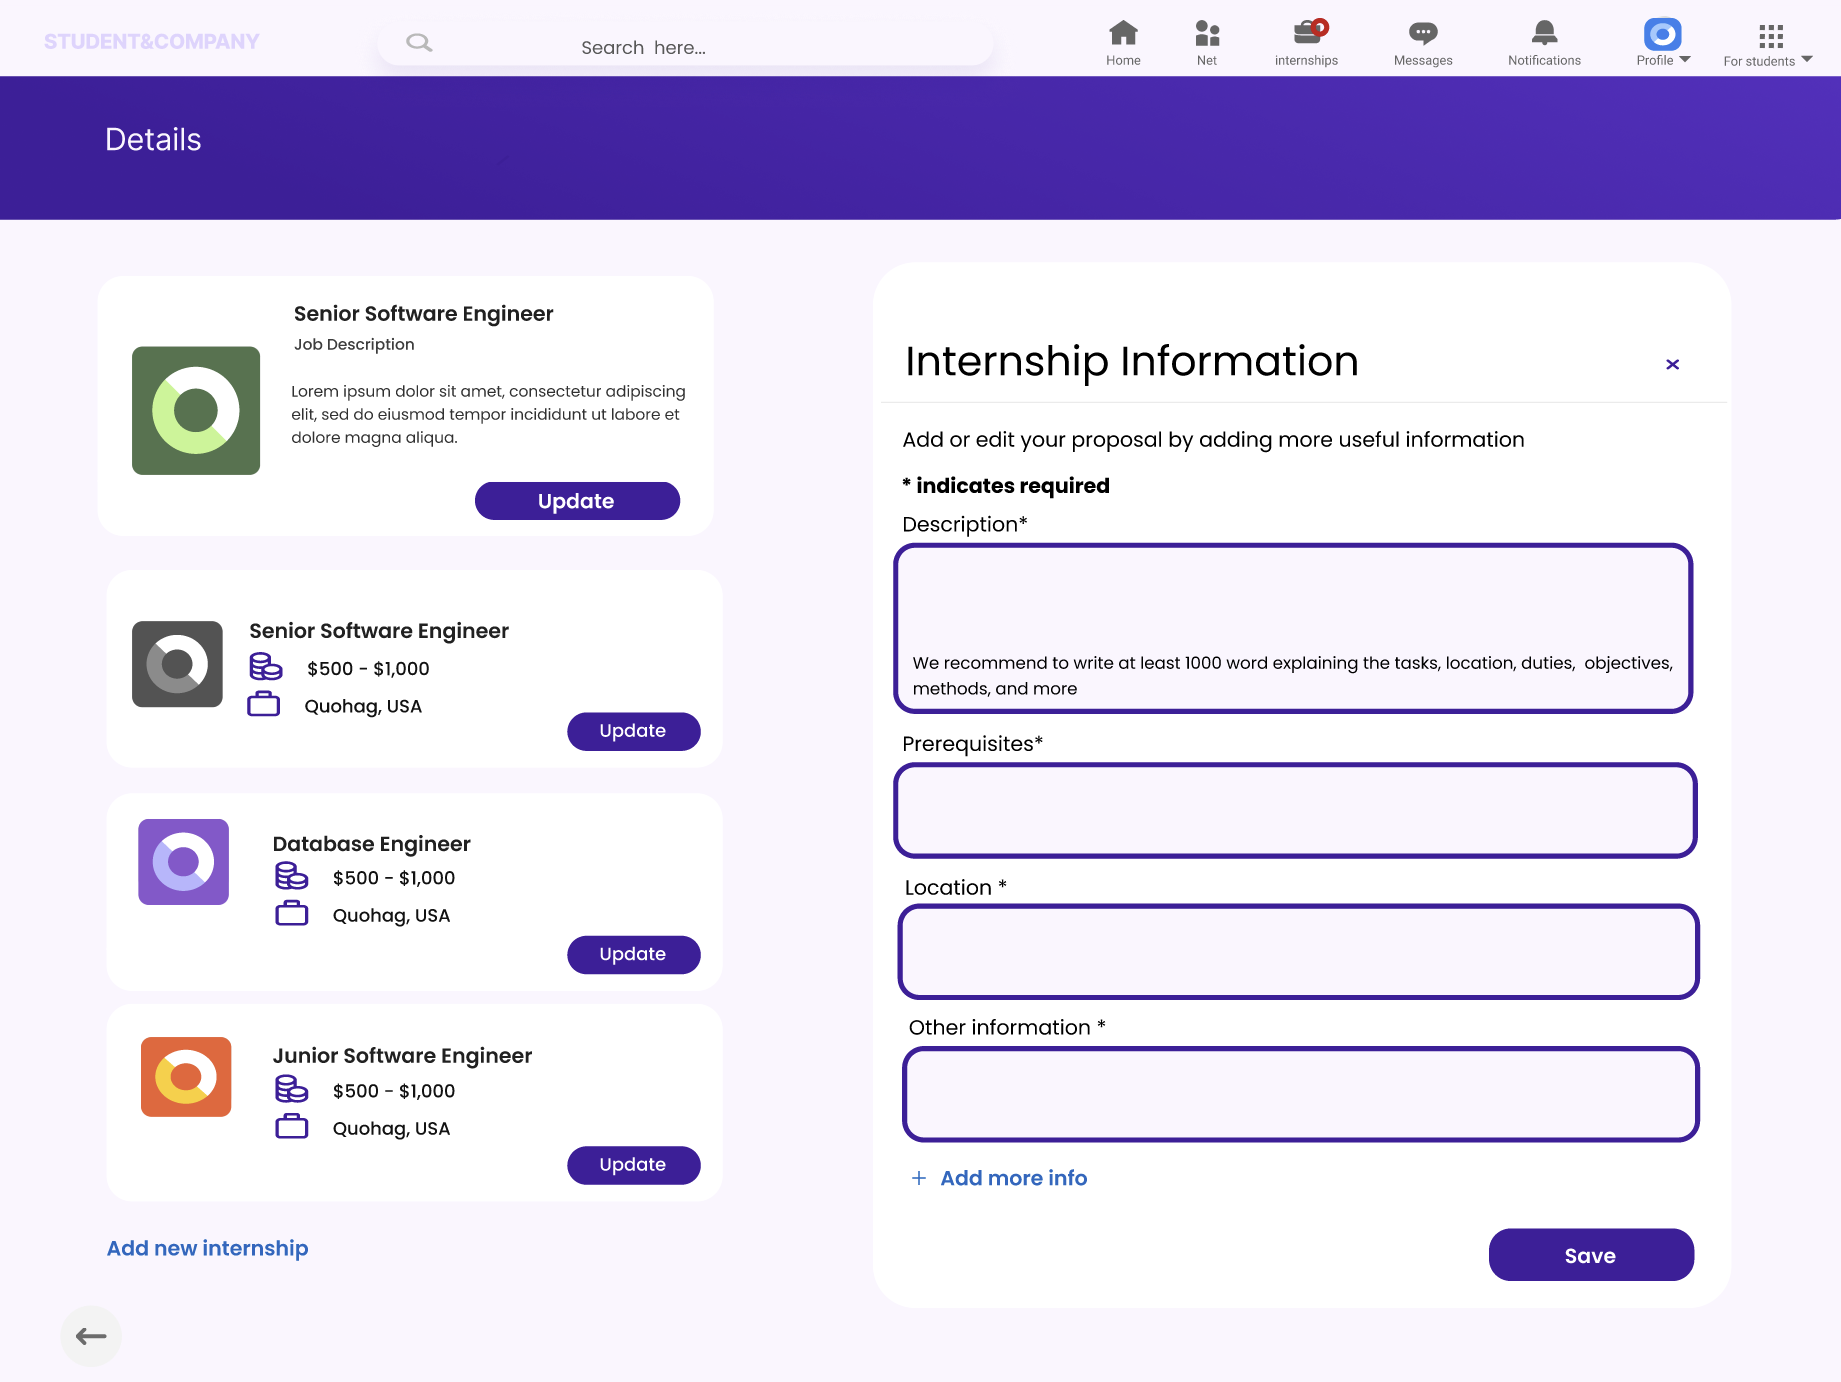
\includegraphics[width=0.5\linewidth]{Images/Interface Images/company interface/Screenshot 2024-12-12 050044.png}
    \caption{Internships management}
    \label{fig:Internships management}
\end{figure}

On the homepage, a company can access the applications section to view all submitted applications. By selecting a specific application, the company can review its details in full, evaluate it positively or negatively, or save it for easier access later [Figure \ref{fig:Application review}] 

\begin{figure} [H]
    \centering
    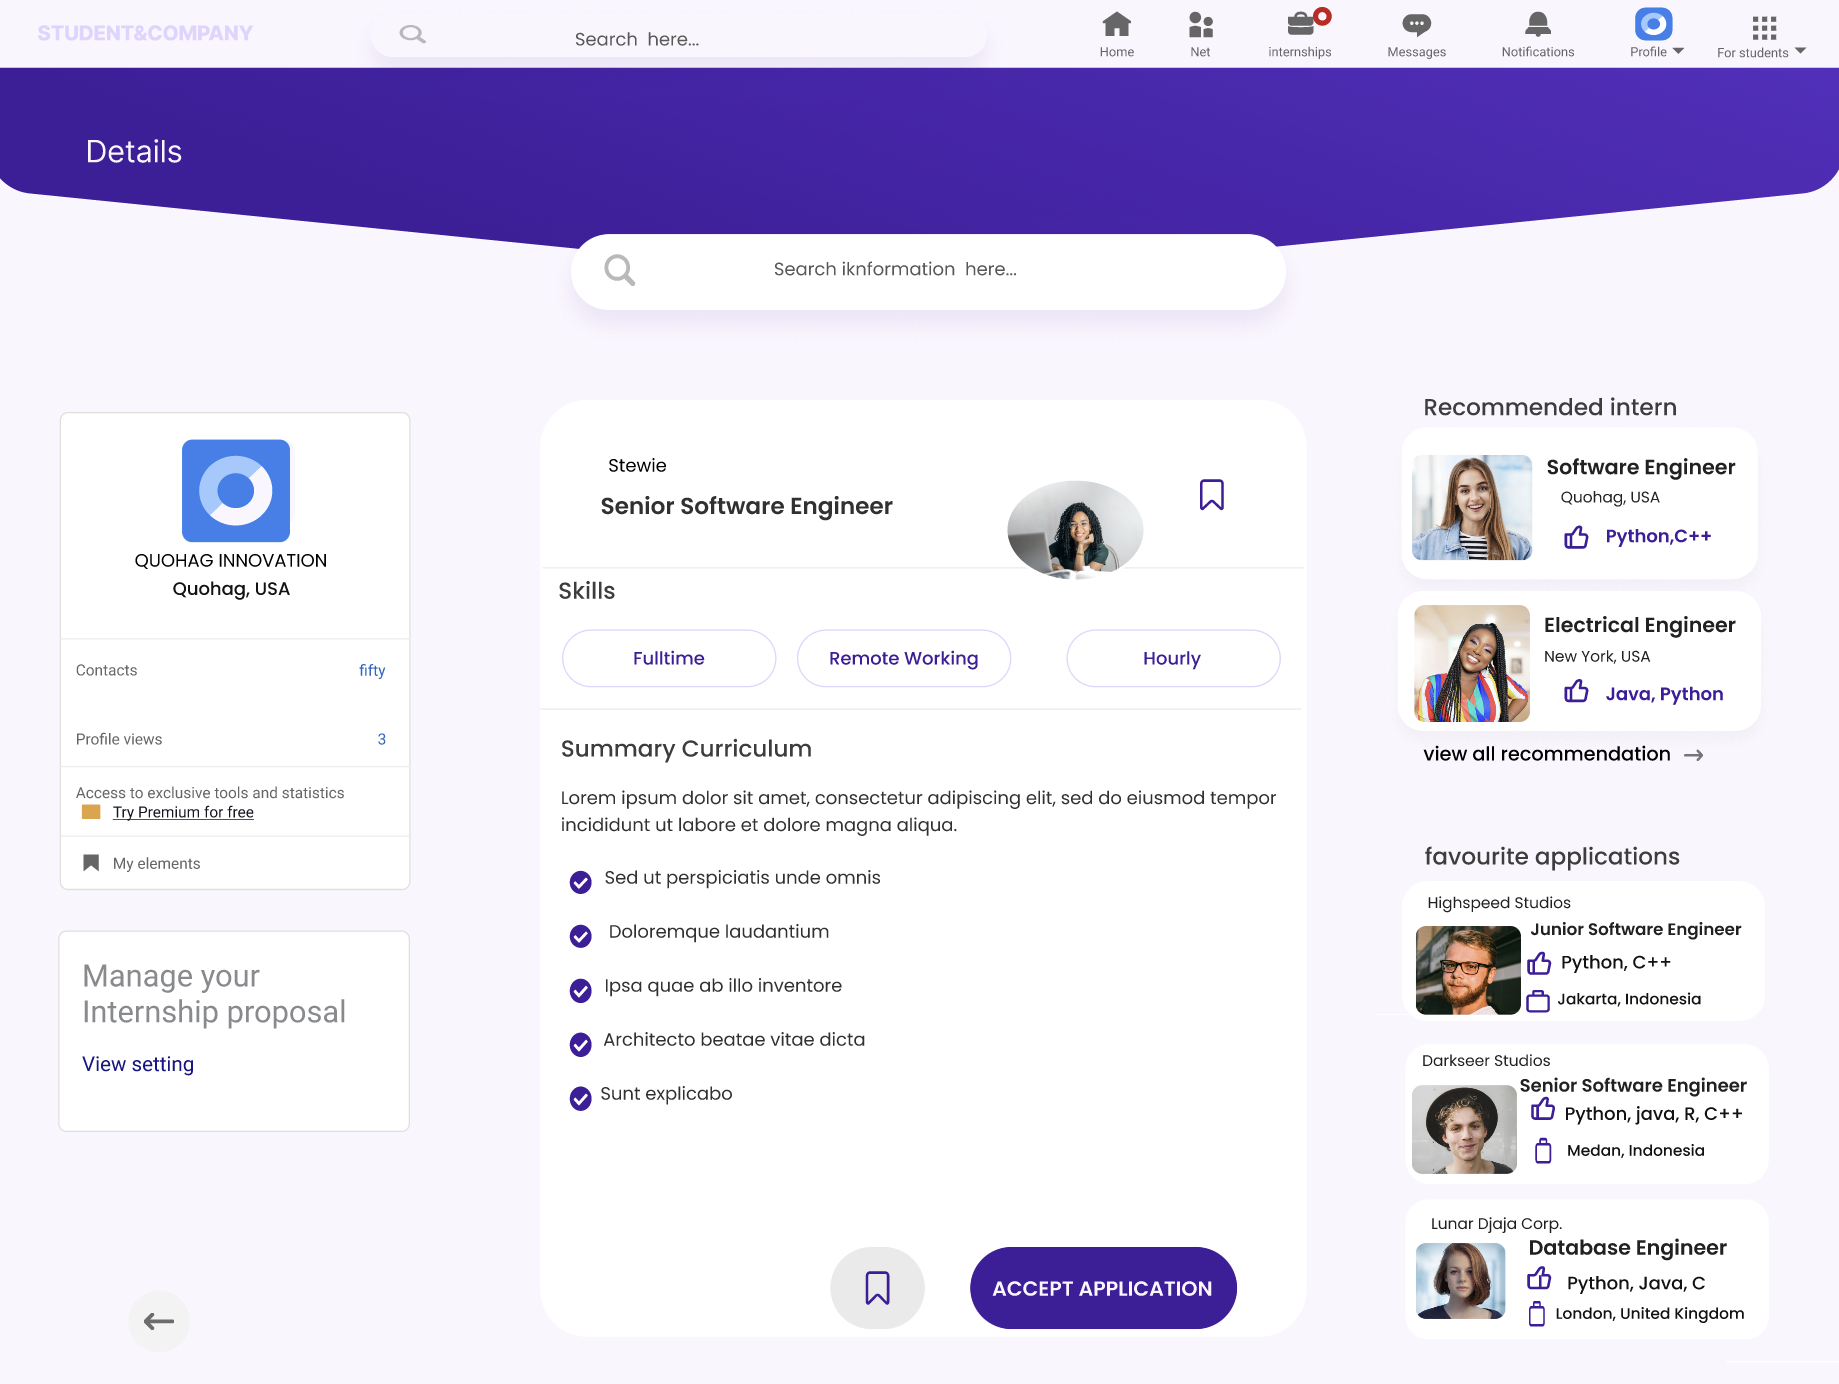
\includegraphics[width=0.5\linewidth]{Images/Interface Images/company interface/Screenshot 2024-12-12 045731.png}
    \caption{Applications review}
    \label{fig:Application review}
\end{figure}


After positively evaluating an application, the company can interview the applicant using a structured questionnaire tailored for each internship proposal. This questionnaire is created by the company and can be enhanced with suggestions provided by the platform [Figure \ref{fig:Interview and questionnaire creation}].

\begin{figure} [H]
    \centering
    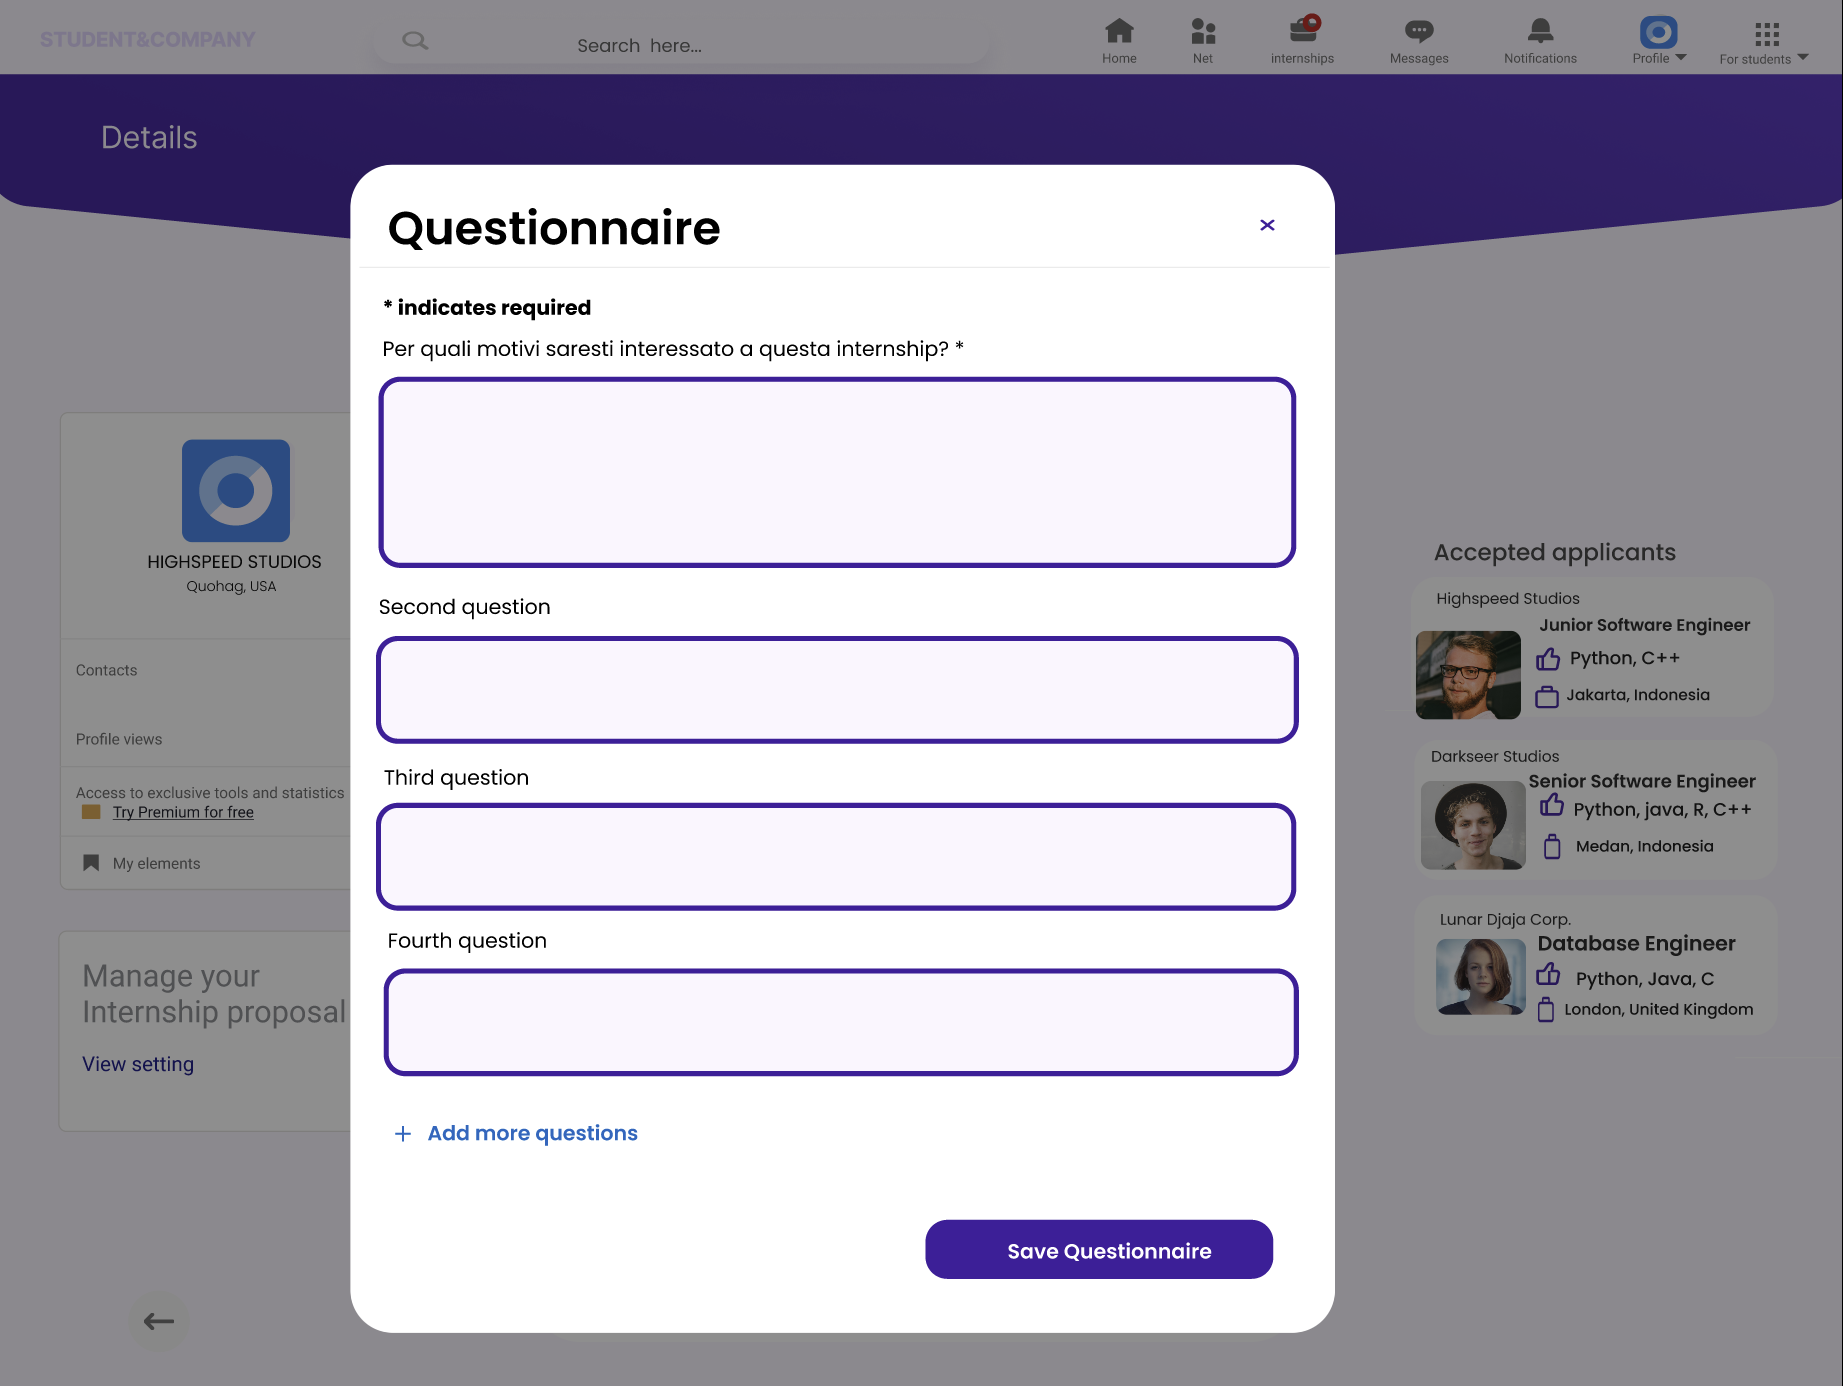
\includegraphics[width=0.5\linewidth]{Images/Interface Images/company interface/Screenshot 2024-12-12 045749.png}
    \caption{Interview and questionnaire creation}
    \label{fig:Interview and questionnaire creation}
\end{figure}

Once a student has completed the questionnaire, the company reviews the submitted answers and evaluates the application. The company can either decline it by providing a negative evaluation or accept it, officially initiating the internship [Figure \ref{fig:Interviews evaluation}].

\begin{figure} [H]
    \centering
    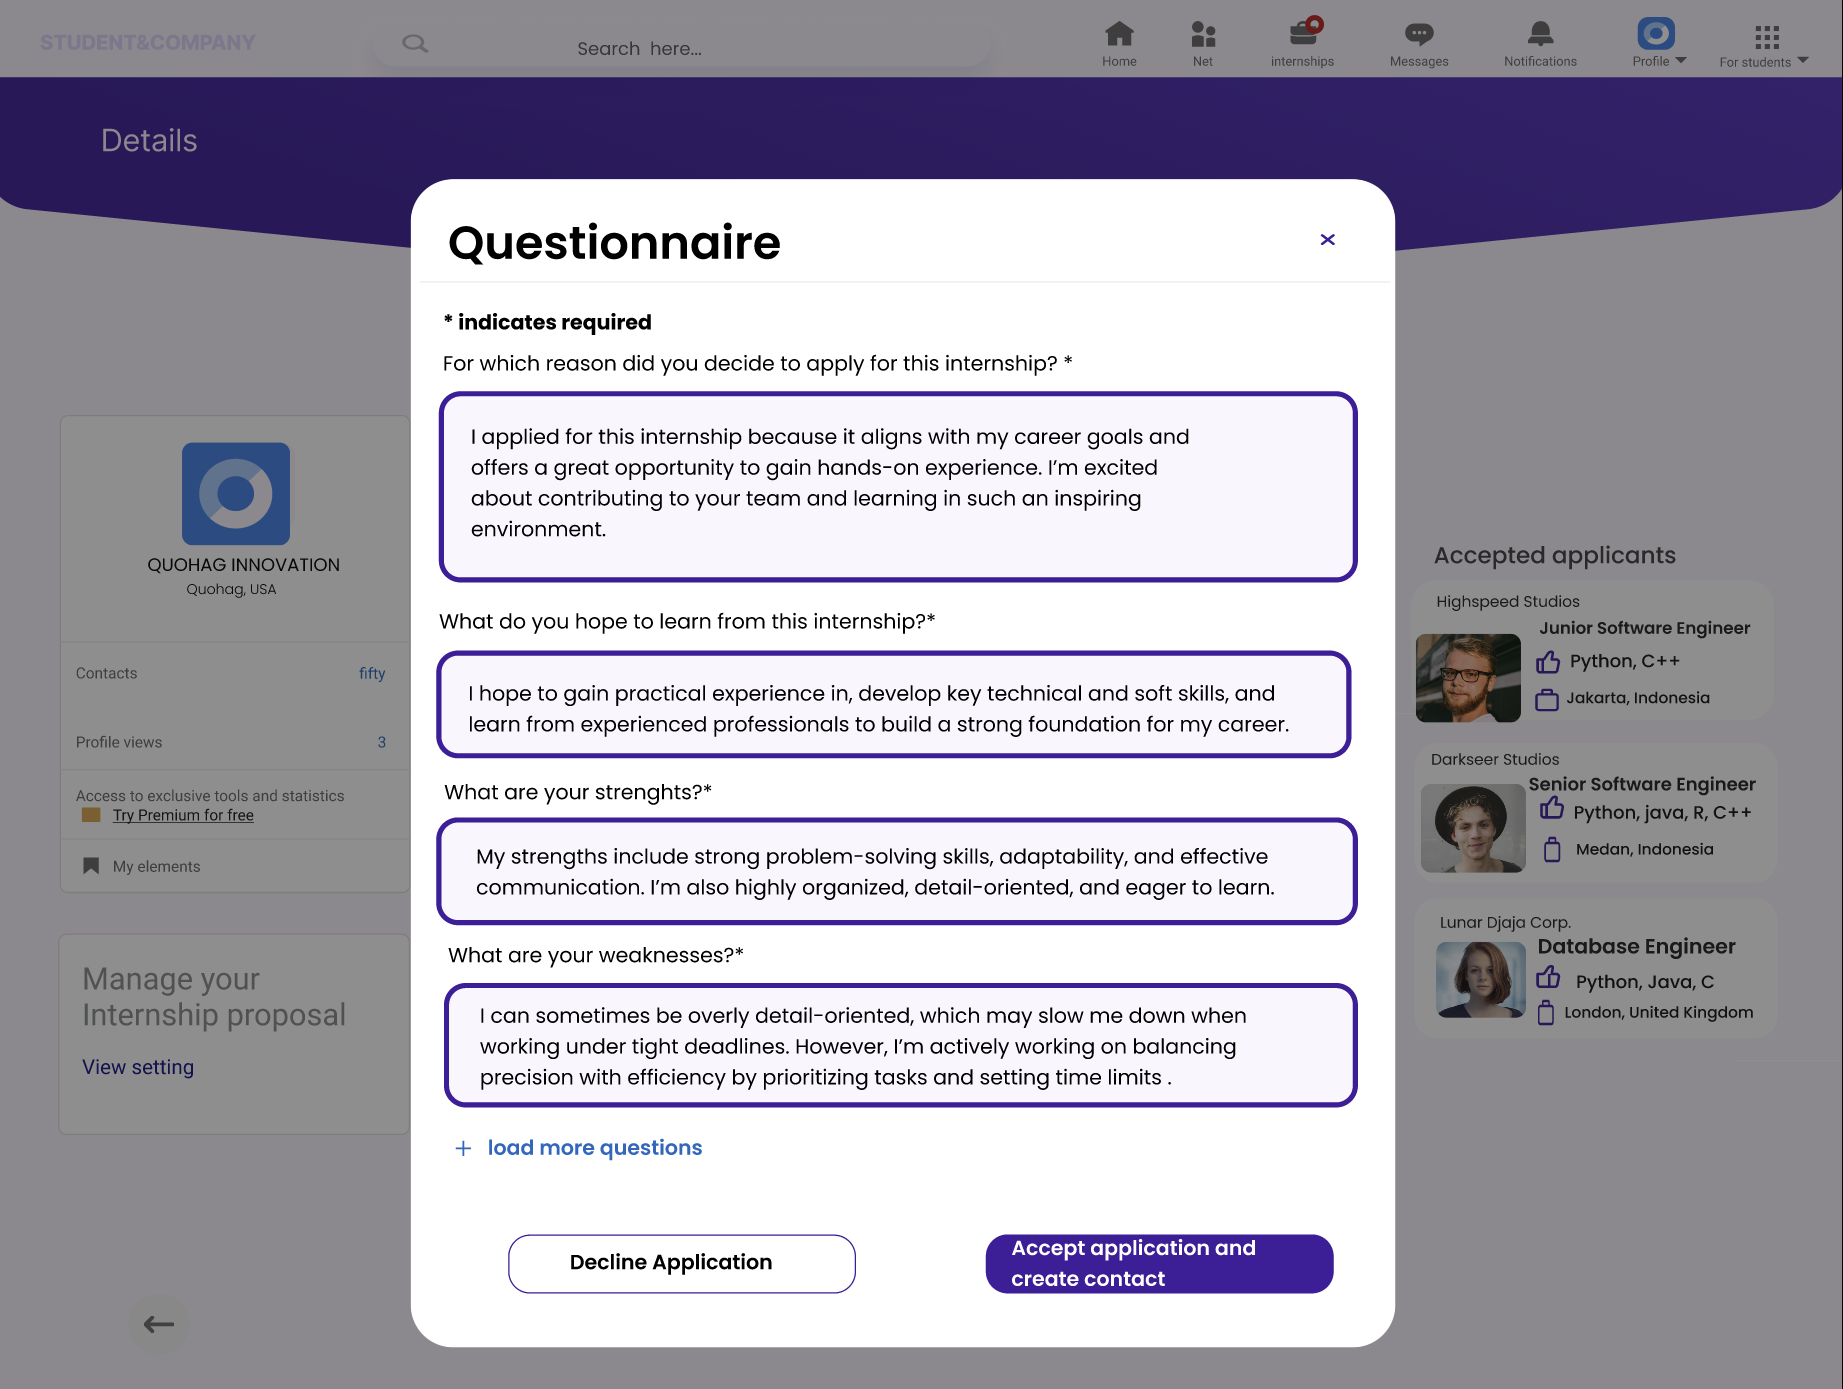
\includegraphics[width=0.5\linewidth]{Images/Interface Images/company interface/Screenshot 2024-12-12 045902.png}
    \caption{Interview evaluation}
    \label{fig:Interviews evaluation}
\end{figure}


\subsection{Student Interfaces}

The student dashboard [Figure \ref{fig:Student Home page}] is the centre of all possible operations on the platform. From this main page, the student can have access to all essential information,
including their personal profile, notifications, available internships, and applications submitted to companies. In addition, it allows the student to communicate with the company after the internship application process is over, as well as provide feedback or submit complaints.

\begin{figure} [H]
    \centering
    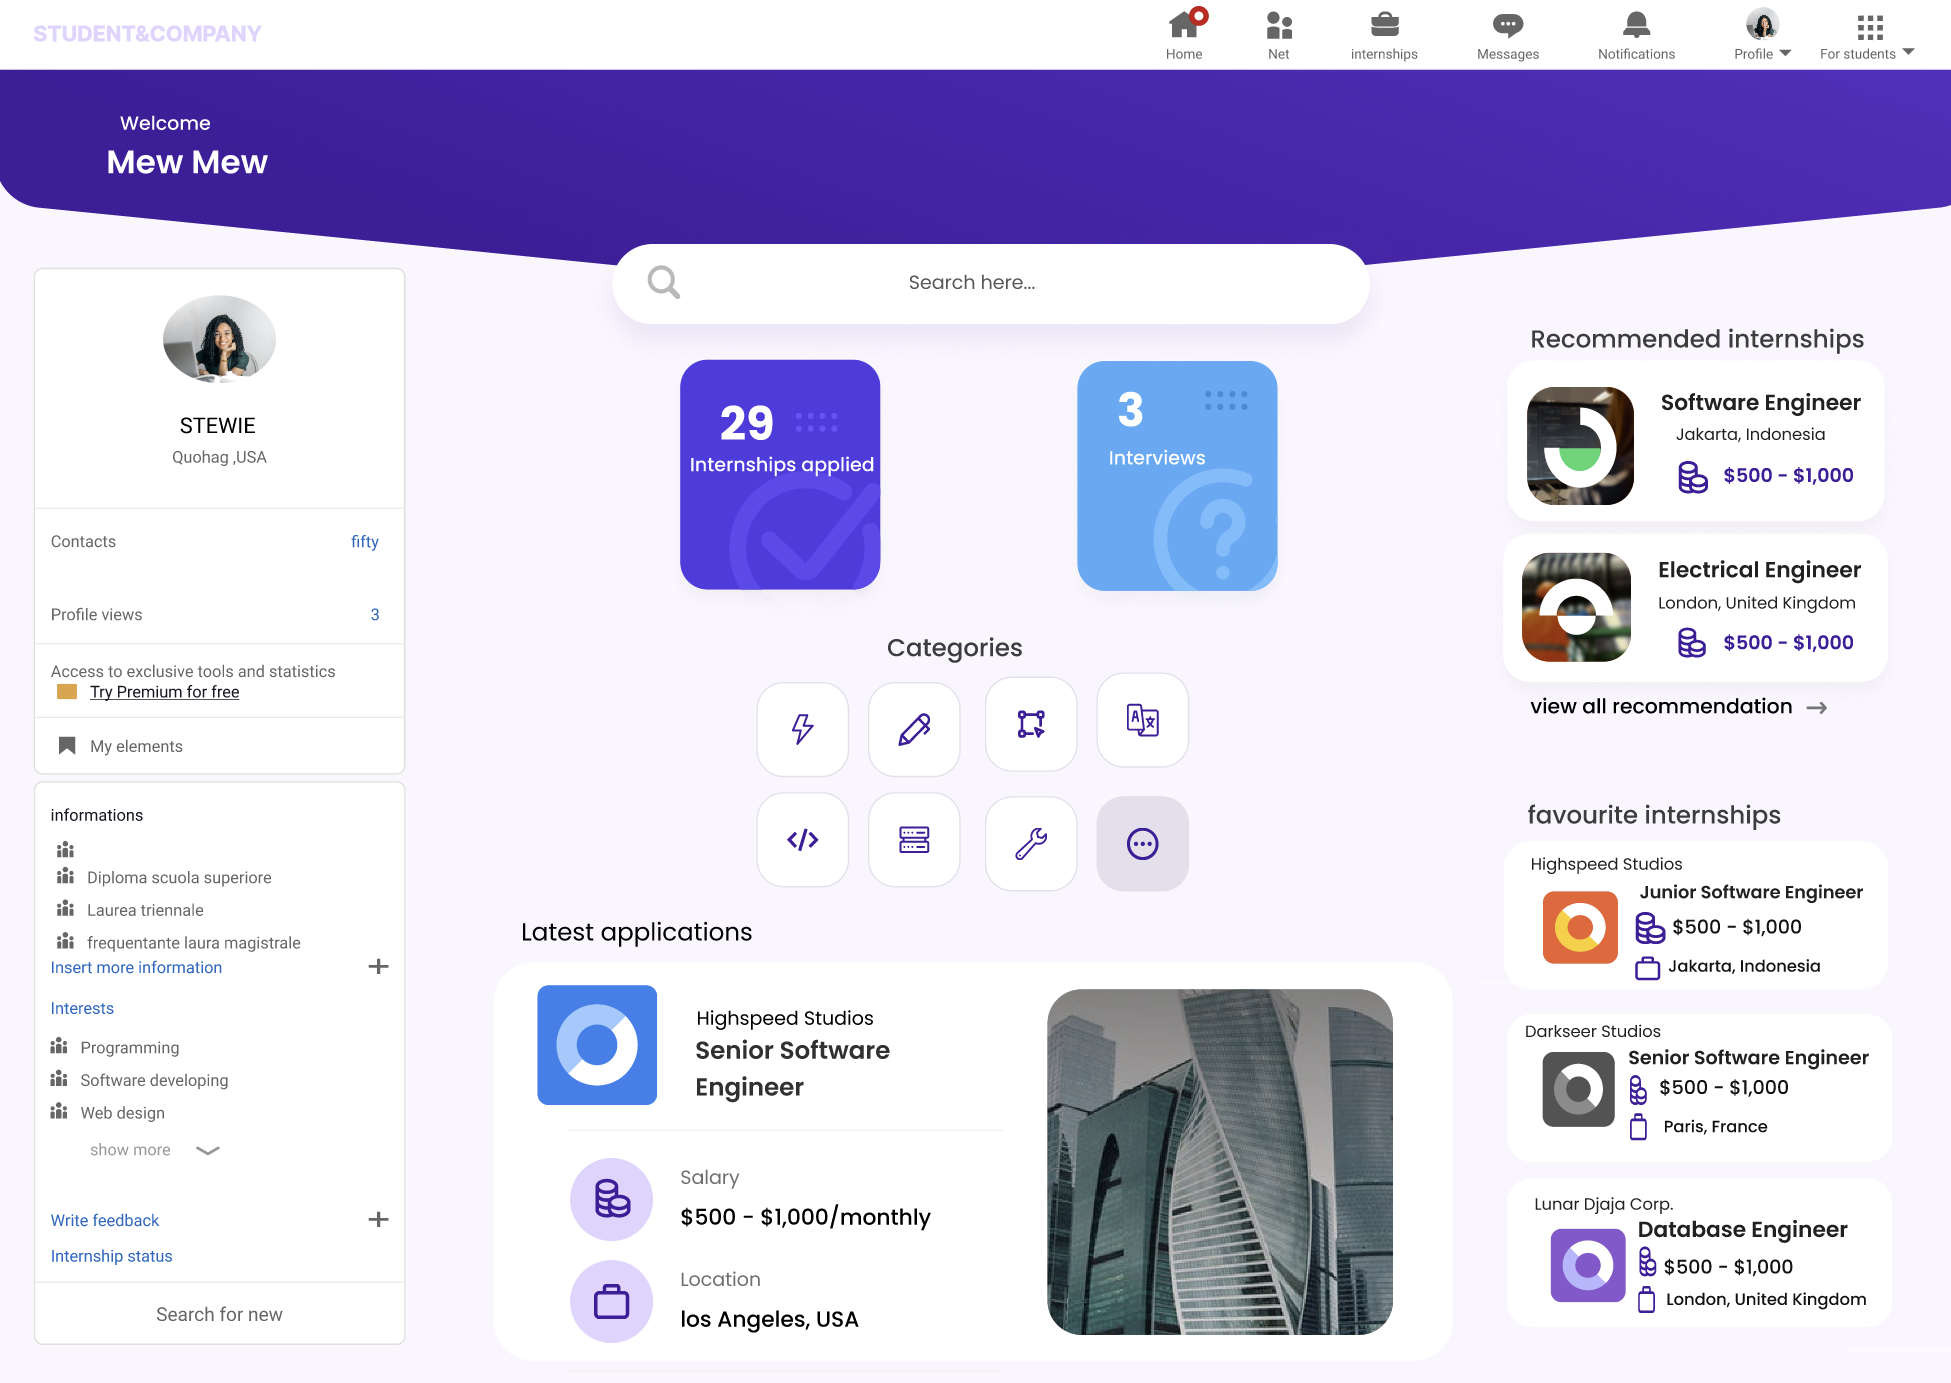
\includegraphics[width=0.5\linewidth]{Images/Interface Images/student interface/Screenshot 2024-12-12 045307.png}
    \caption{Student Home page}
    \label{fig:Student Home page}
\end{figure}

In the personal profile section, students can input their personal details as well as information relevant to creating a CV for internship applications. Students have the option to enter this information independently or follow platform suggestions and tips to enhance their CV, making it more appealing to potential employers. The information is organized into sections and will be visible to companies later on.

\begin{figure} [H]
    \centering
    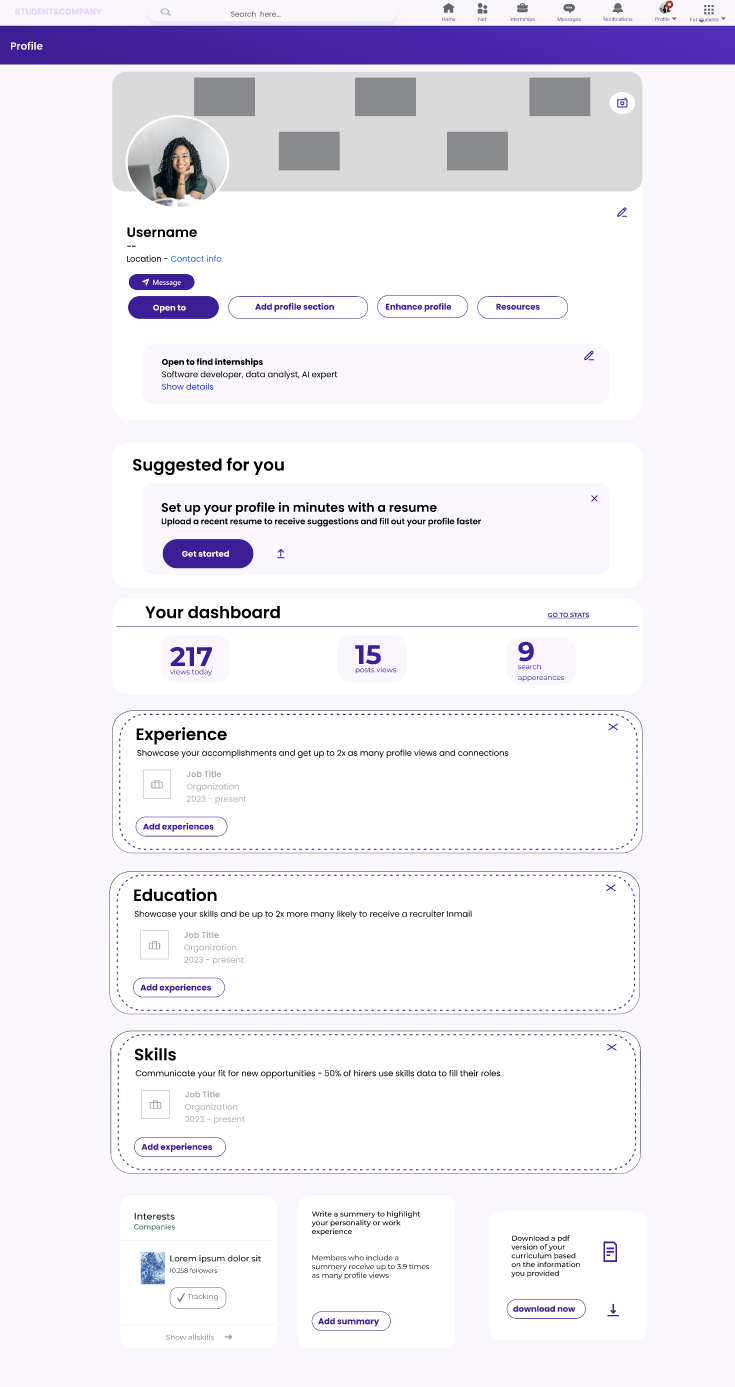
\includegraphics[width=0.5\linewidth]{Images/Interface Images/student interface/Screenshot 2024-12-12 045421.png}
    \caption{Student Personal profile}
    \label{fig:Student Personal profile}
\end{figure}

\begin{figure} [H]
    \centering
    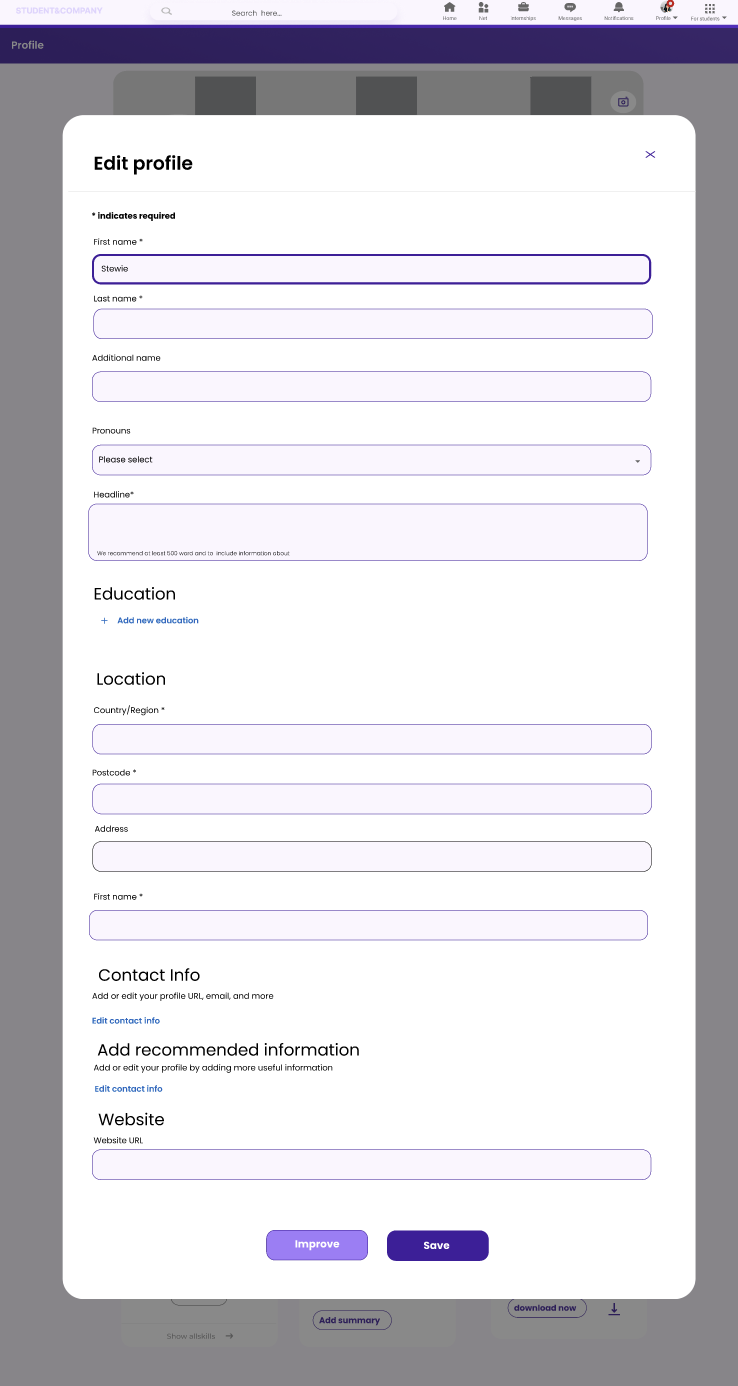
\includegraphics[width=0.5\linewidth]{Images/Interface Images/student interface/Screenshot 2024-12-12 045447.png}
    \caption{Student Profile management}
    \label{fig:Student Profile management}
\end{figure}


In the search section, students can explore all available internships on the platform. To make the search more relevant and tailored to their personal interests, several filters are provided, allowing students to select internships based on criteria they specify. The internships will be displayed in a list, showing only key details. By clicking on a specific internship, students can view all the information and find the option to apply if they're interested in that particular opportunity.

\begin{figure} [H]
    \centering
    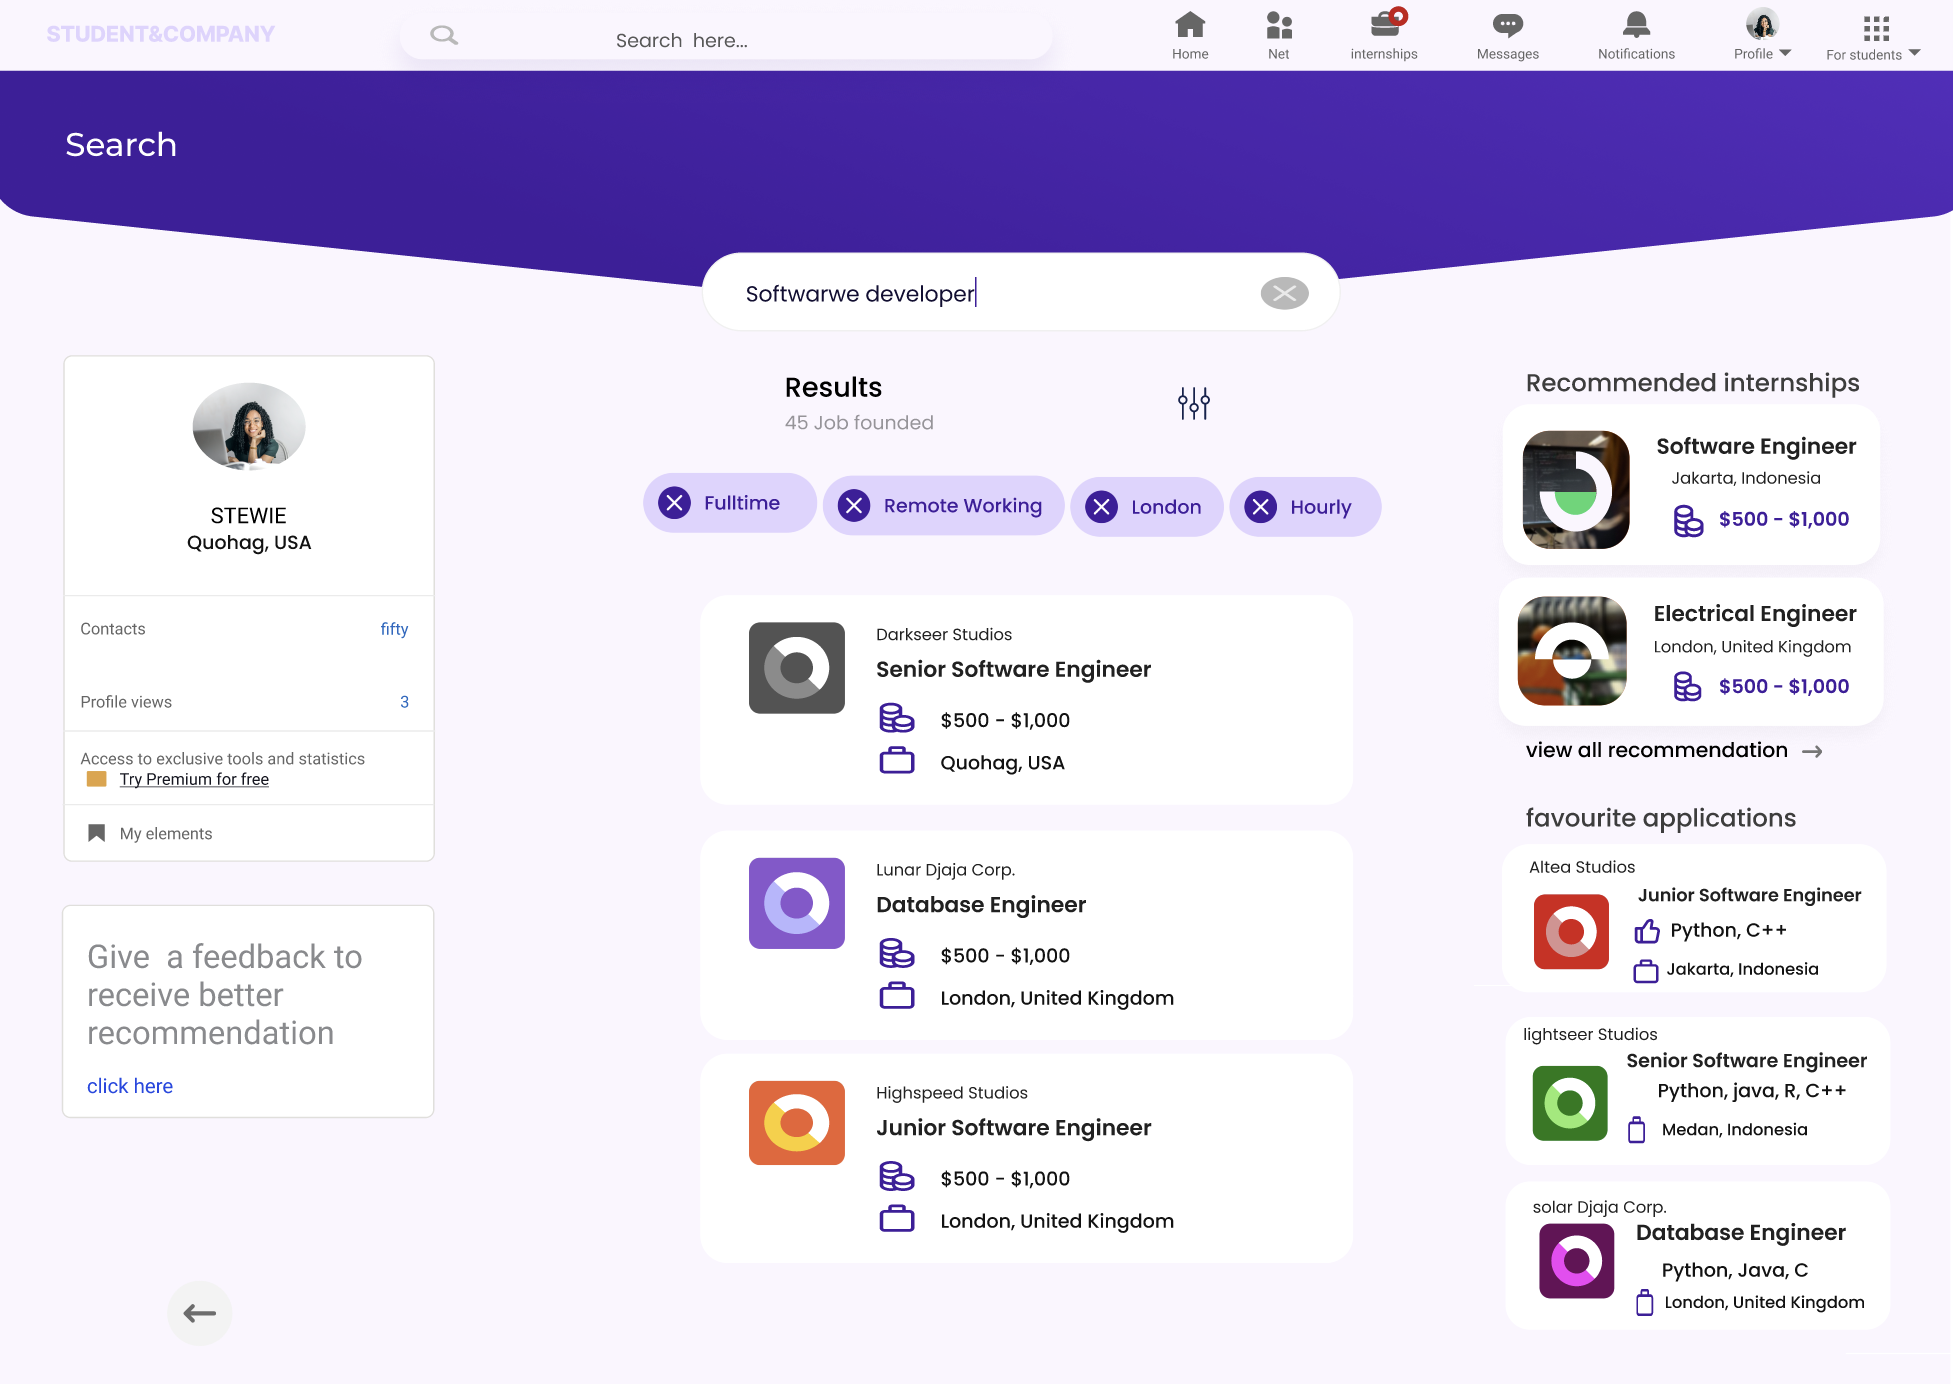
\includegraphics[width=0.5\linewidth]{Images/Interface Images/student interface/Screenshot 2024-12-12 045606.png}
    \caption{Internships lookup}
    \label{fig: Internships lookup}
\end{figure}

\begin{figure} [H]
    \centering
    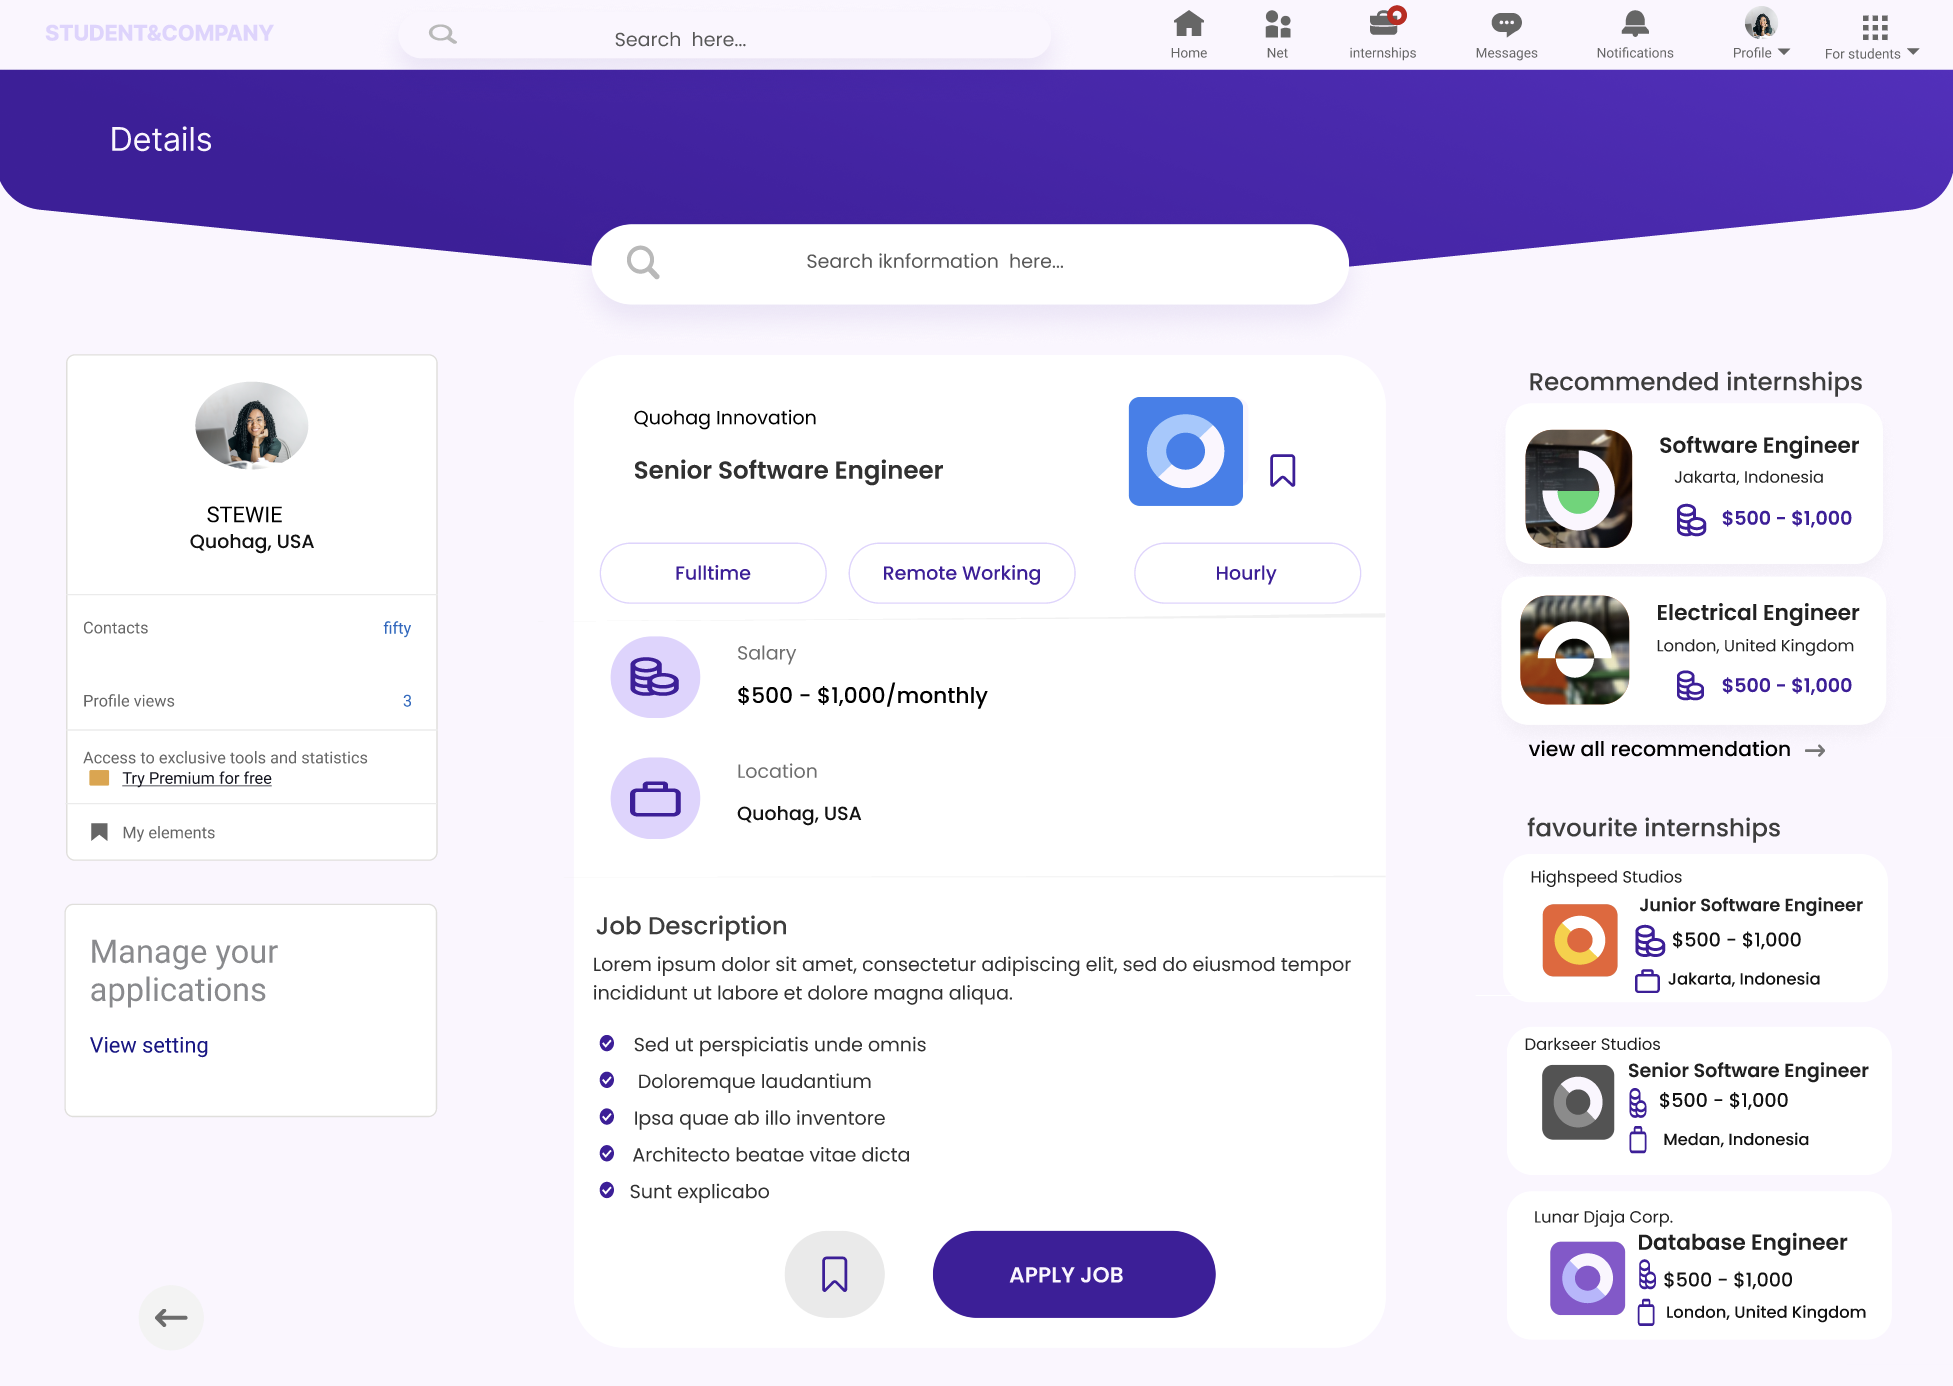
\includegraphics[width=0.5\linewidth]{Images/Interface Images/student interface/Screenshot 2024-12-12 045619.png}
    \caption{Internship details}
    \label{fig:Internship details}
\end{figure}

After clicking the "Apply" button, the student can proceed with the internship application. To complete the application, the student must either upload their CV or consent to share their personal profile information with the company. Additionally, the student will need to provide other personal details, such as their name, surname, and email. Once all the required information is submitted, the student can send the application.

\begin{figure} [H]
    \centering
    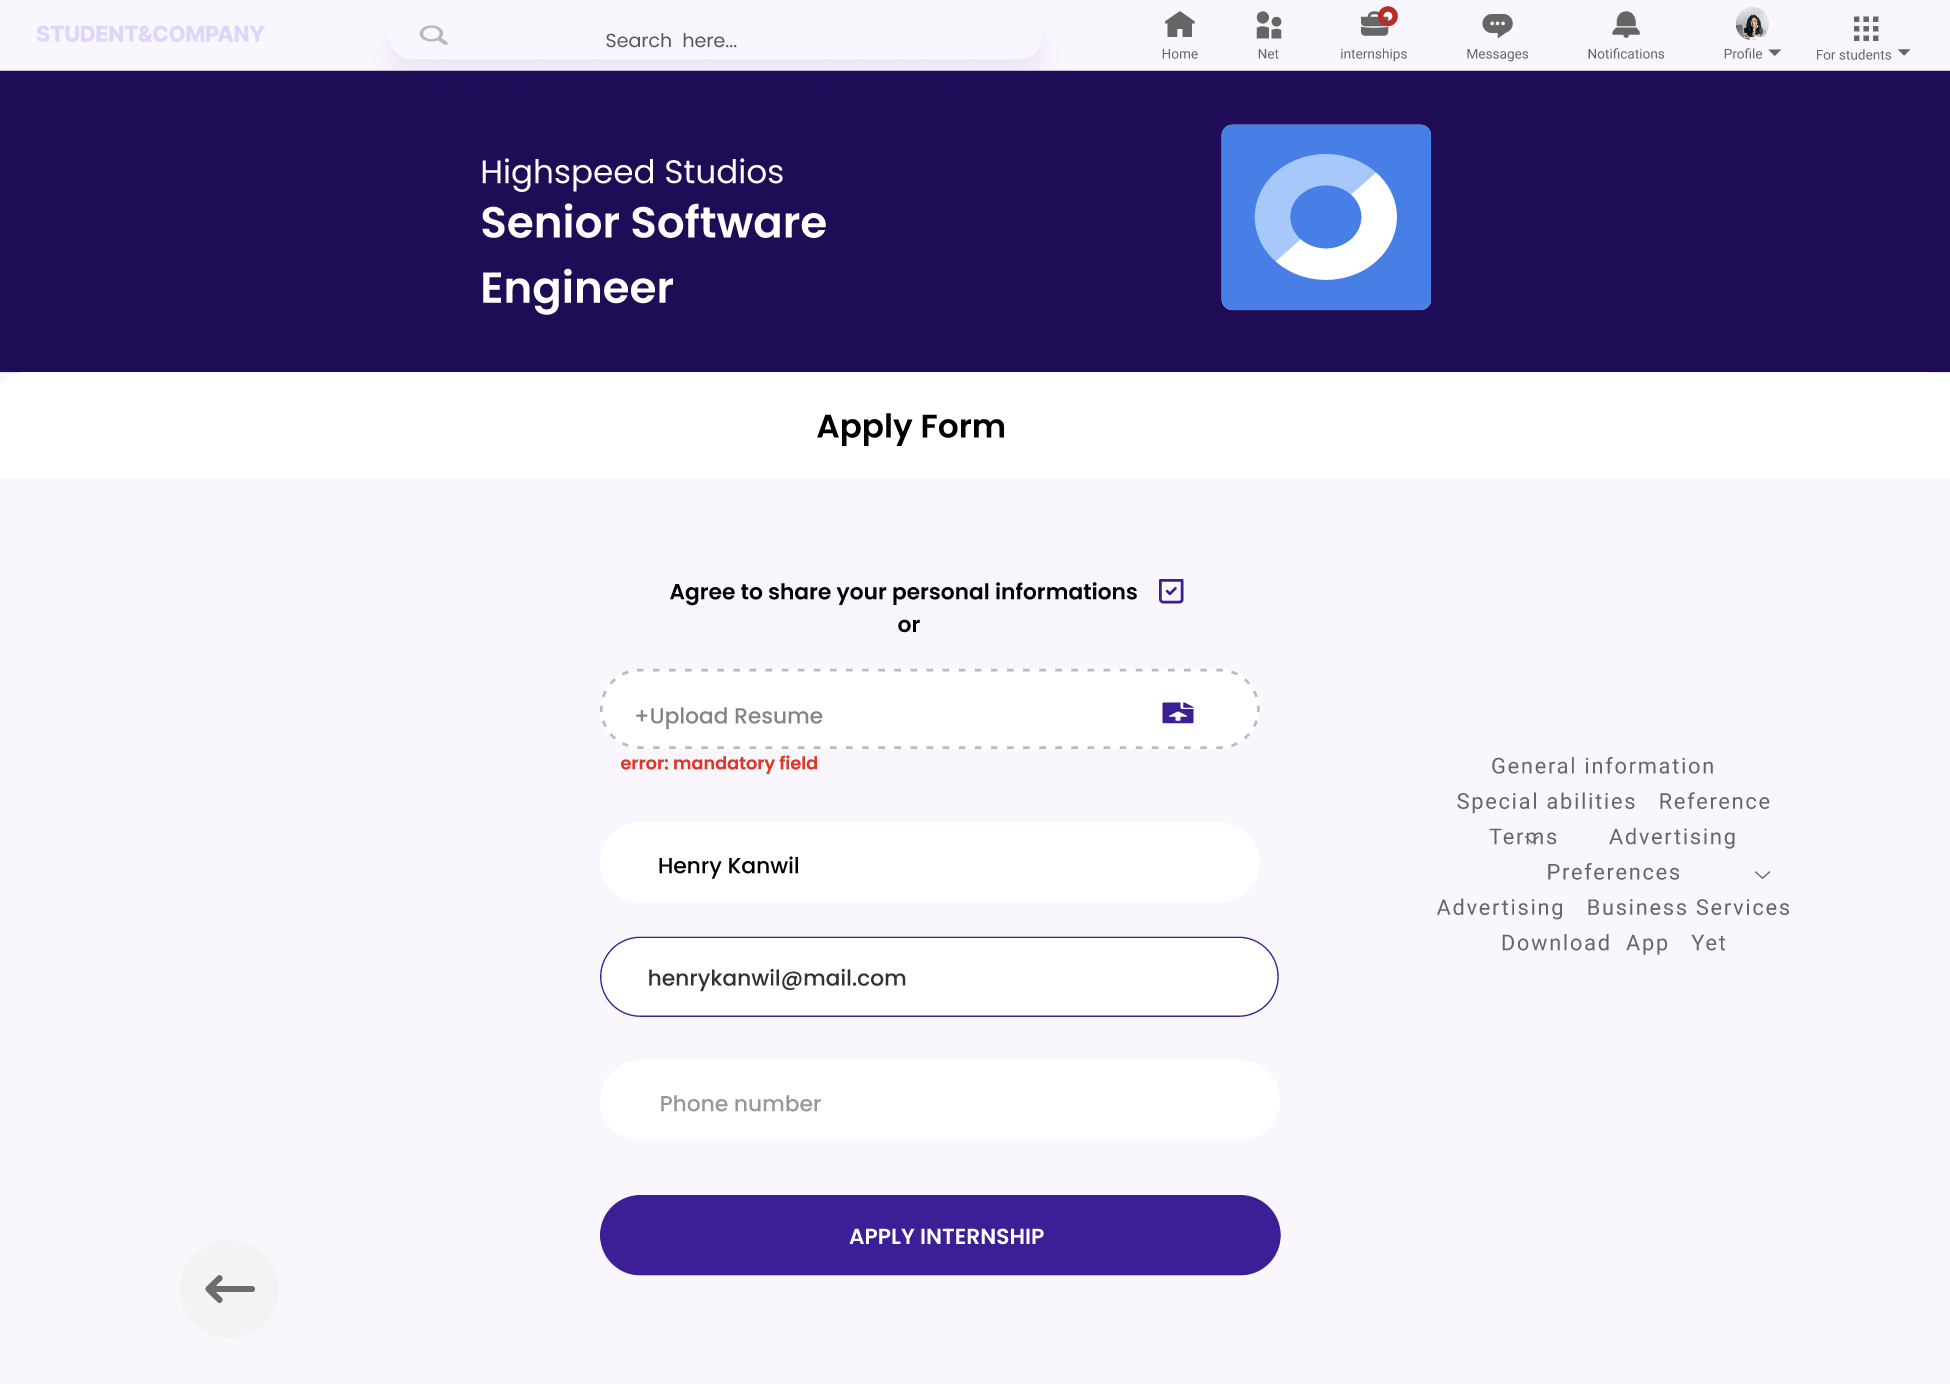
\includegraphics[width=0.5\linewidth]{Images/Interface Images/student interface/Screenshot 2024-12-12 045639.png}
    \caption{Application form}
    \label{fig:Application form}
\end{figure}

Once an application is submitted and a positive evaluation is received, the interview section will become available on the internship page. The interview is structured as a questionnaire, which is pre-prepared by the company for each specific internship. The student must answer all questions in the questionnaire before submitting it back to the company for final evaluation. Based on this evaluation, the company will make the final decision on whether to proceed with the internship.


\begin{figure} [H]
    \centering
    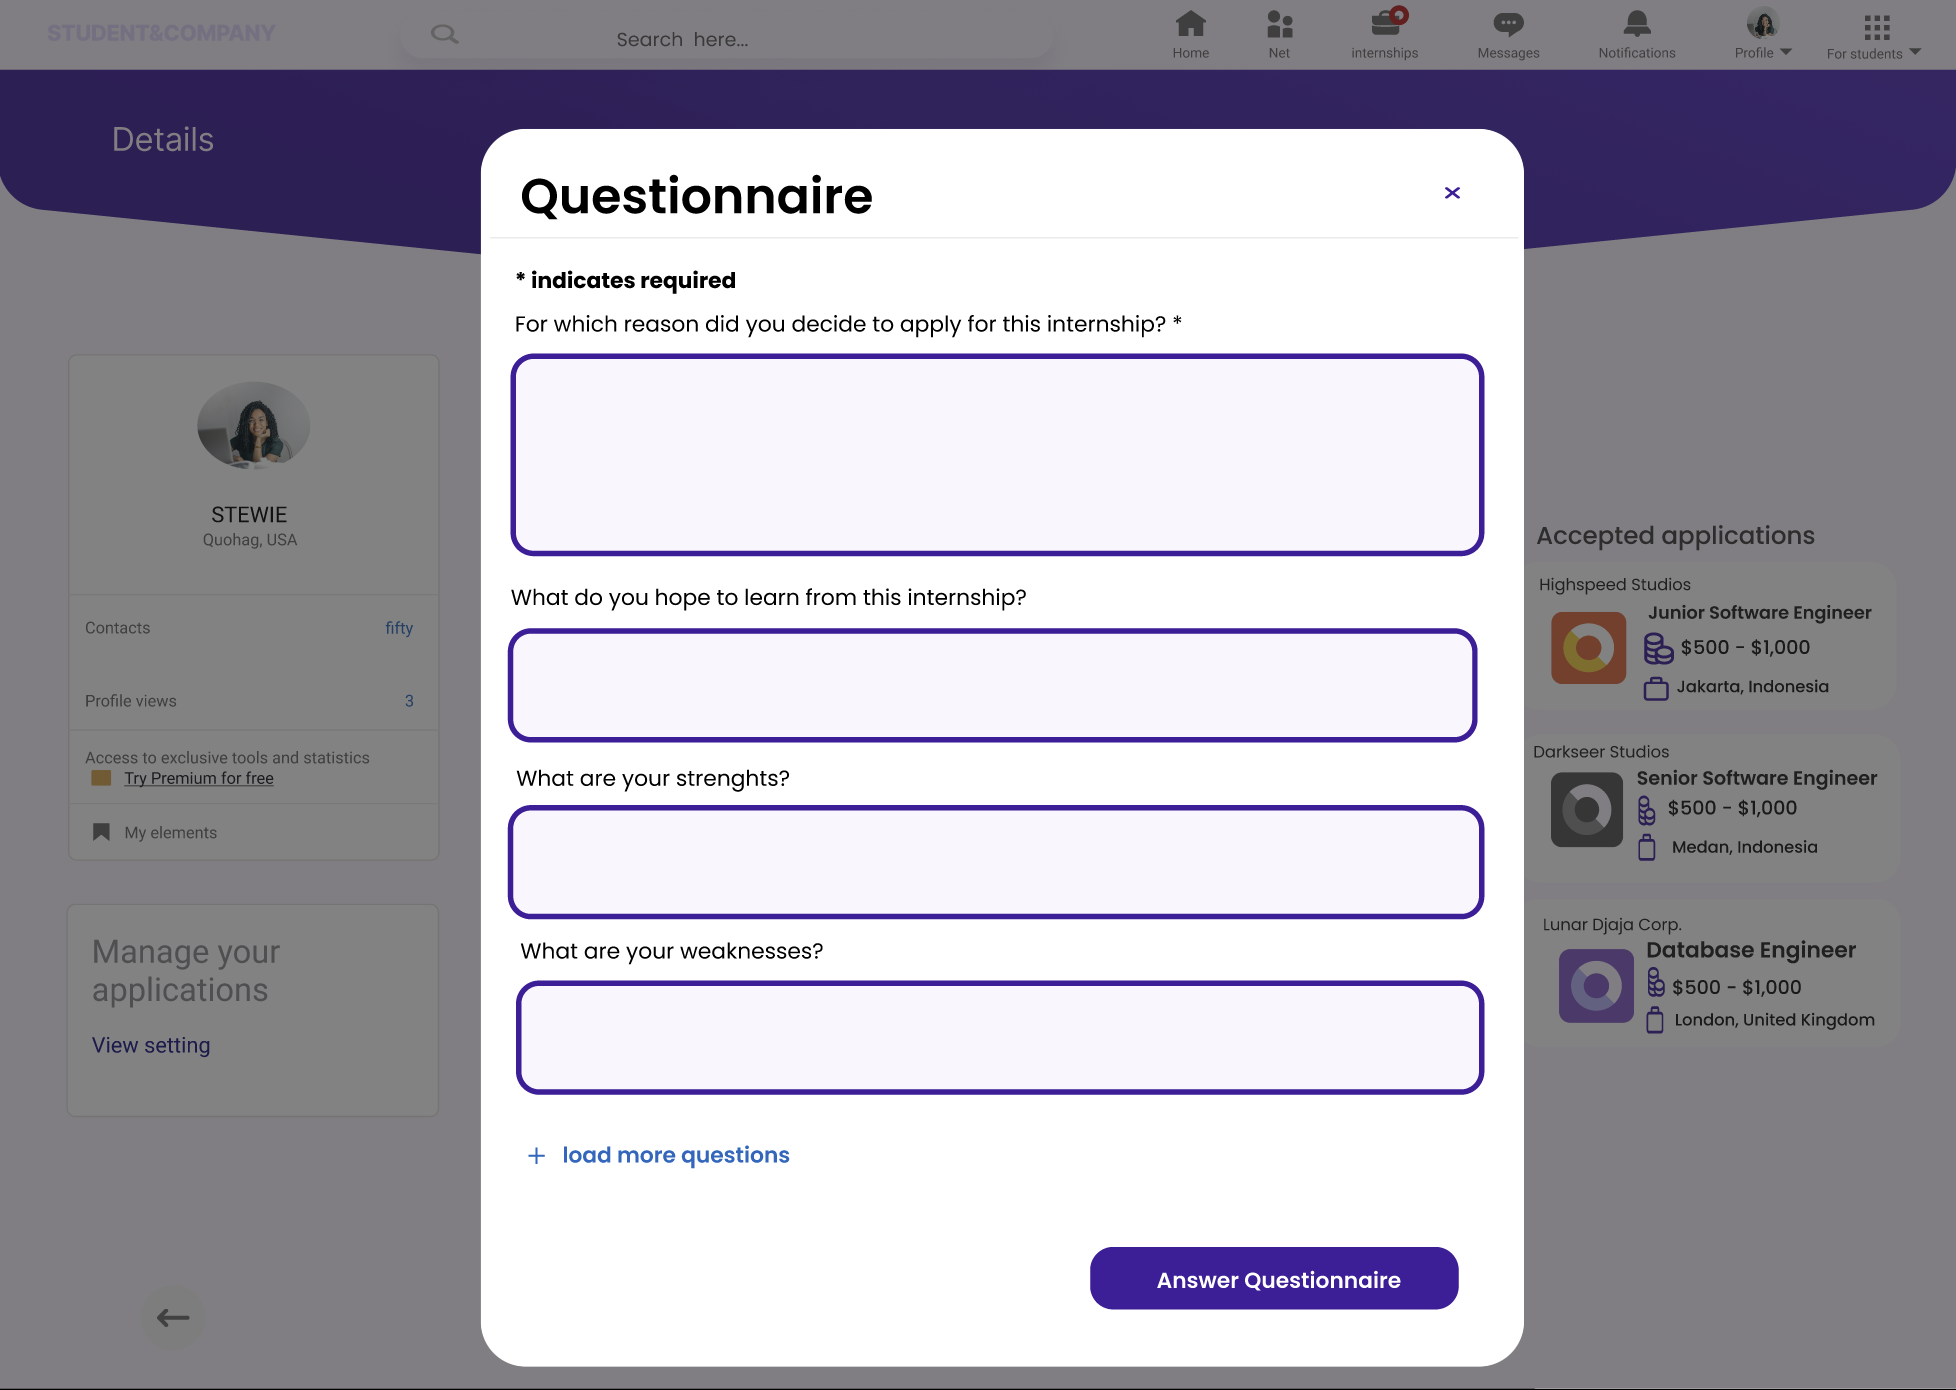
\includegraphics[width=0.5\linewidth]{Images/Interface Images/student interface/Screenshot 2024-12-12 045852.png}
    \caption{Interview reply}
    \label{fig:Interview reply}
\end{figure}

Throughout the application process, the student will be able to monitor the status of their application and receive notifications whenever there is a change. The status will update based on different stages, including: application sent, awaiting review, evaluated negatively, evaluated positively, interview ready, interview submitted, and interview evaluated.

\begin{figure} [H]
    \centering
    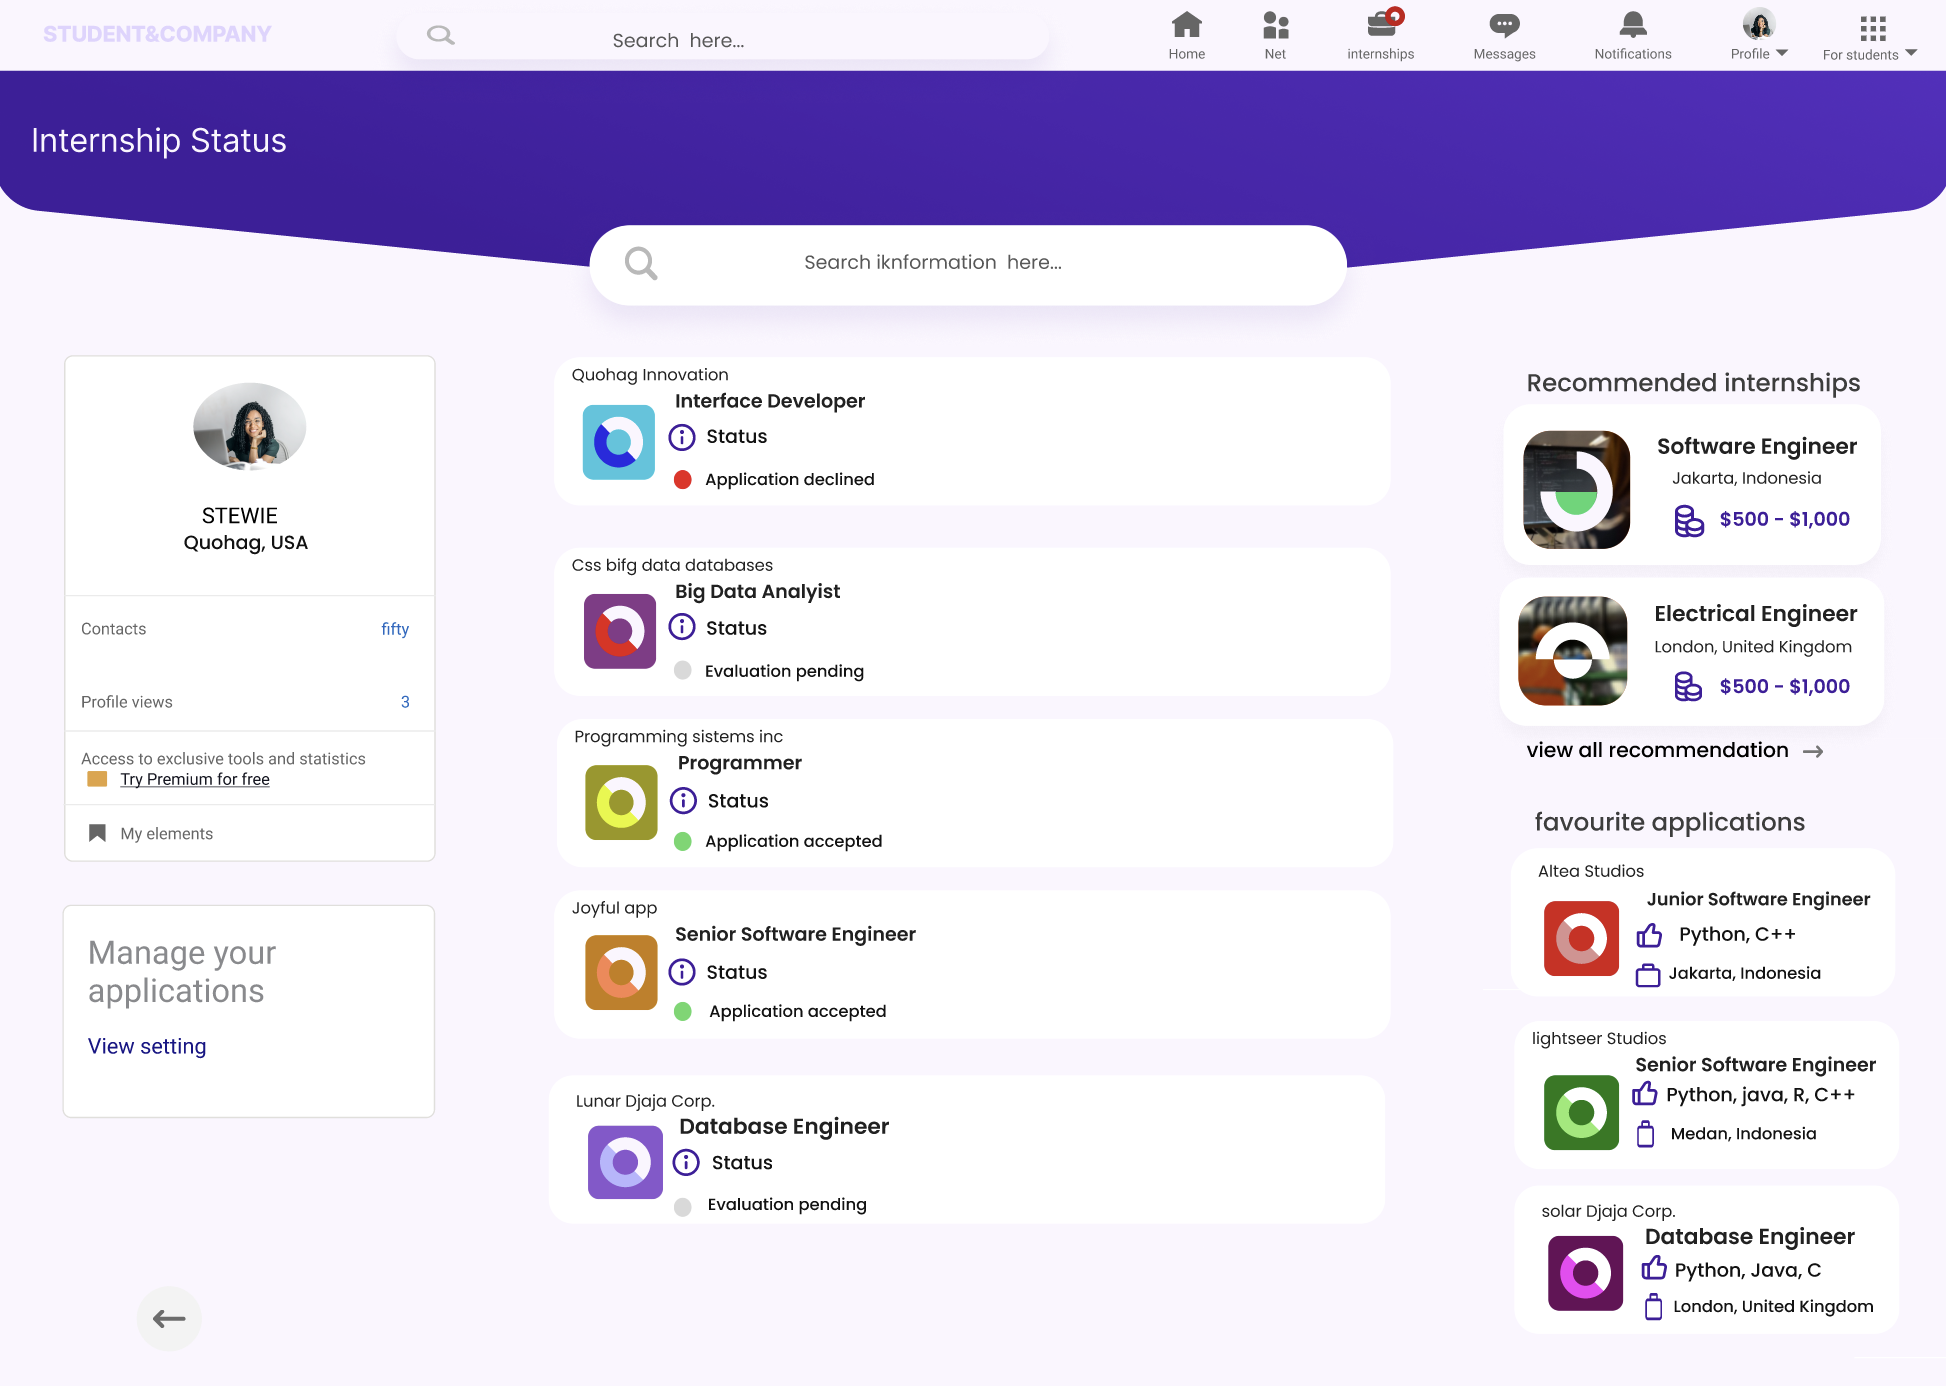
\includegraphics[width=0.5\linewidth]{Images/Interface Images/student interface/Screenshot 2024-12-12 050031.png}
    \caption{Application status}
    \label{fig:Application status}
\end{figure}

\subsection{University Interfaces}


The university's Dashboard [Figure \ref{fig: University Home page}] serves as the central hub for all platform operations. From this main page, the university can easily access essential information, including its notifications the personal profiles of the students enrolled, and all complaints sent by both students and companies. Additionally, it allows the university to communicate with students and companies after a complaint has been submitted, allowing for a better resolution of the problems.

\begin{figure} [H]
    \centering
    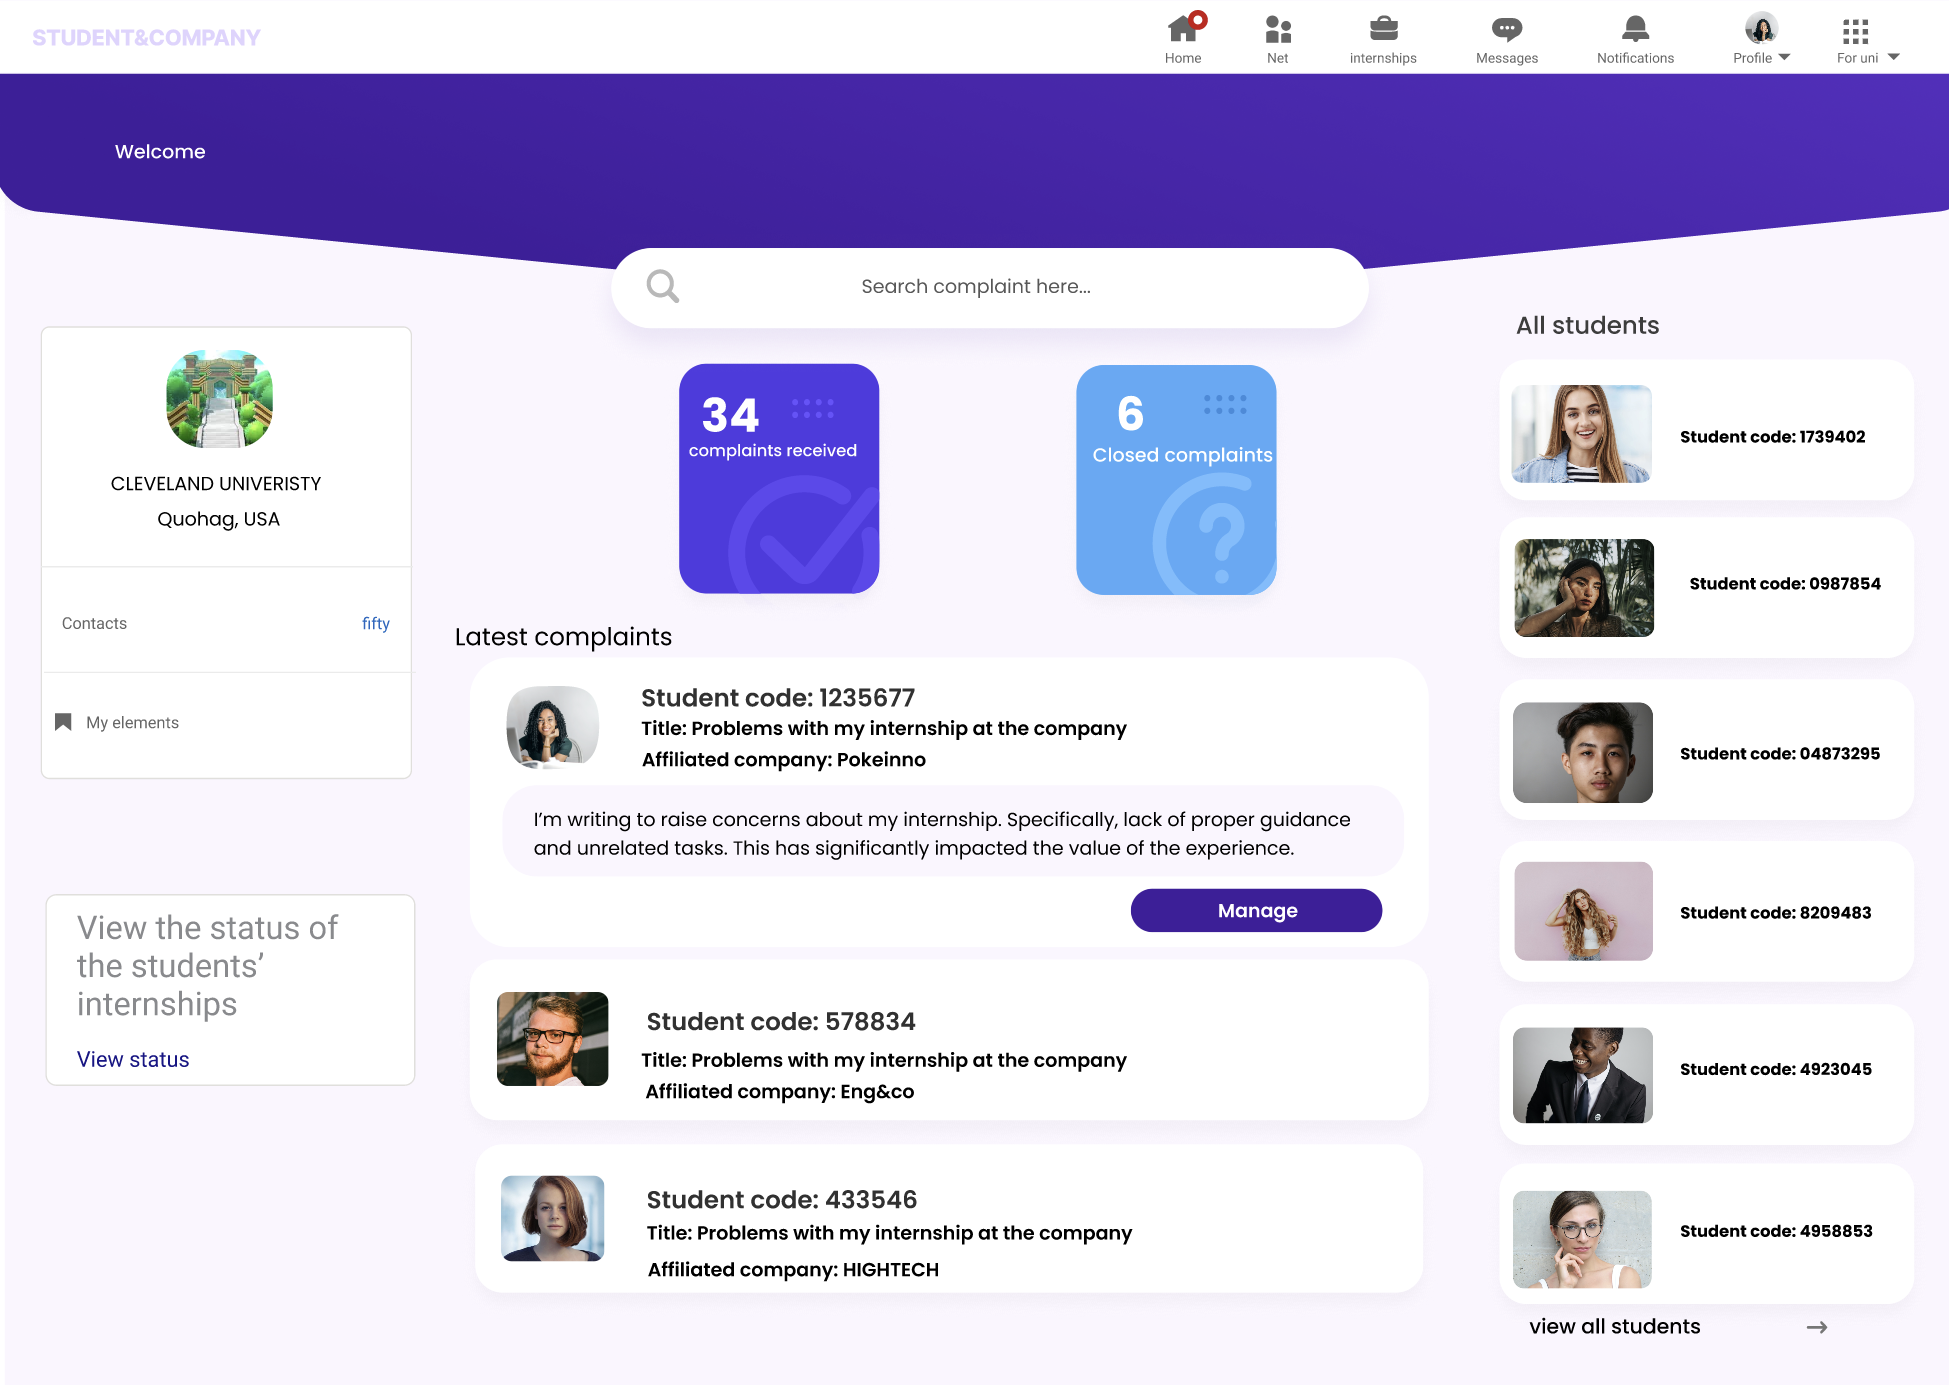
\includegraphics[width=0.5\linewidth]{Images/Interface Images/university interface/Screenshot 2024-12-12 045335.png}
    \caption{University Home page}
    \label{fig: University Home page}
\end{figure}


By clicking on a complaint, the university can respond directly by sending a reply message to the user who submitted it [Figure \ref{fig:Complaints visualization}].

\begin{figure} [H]
    \centering
    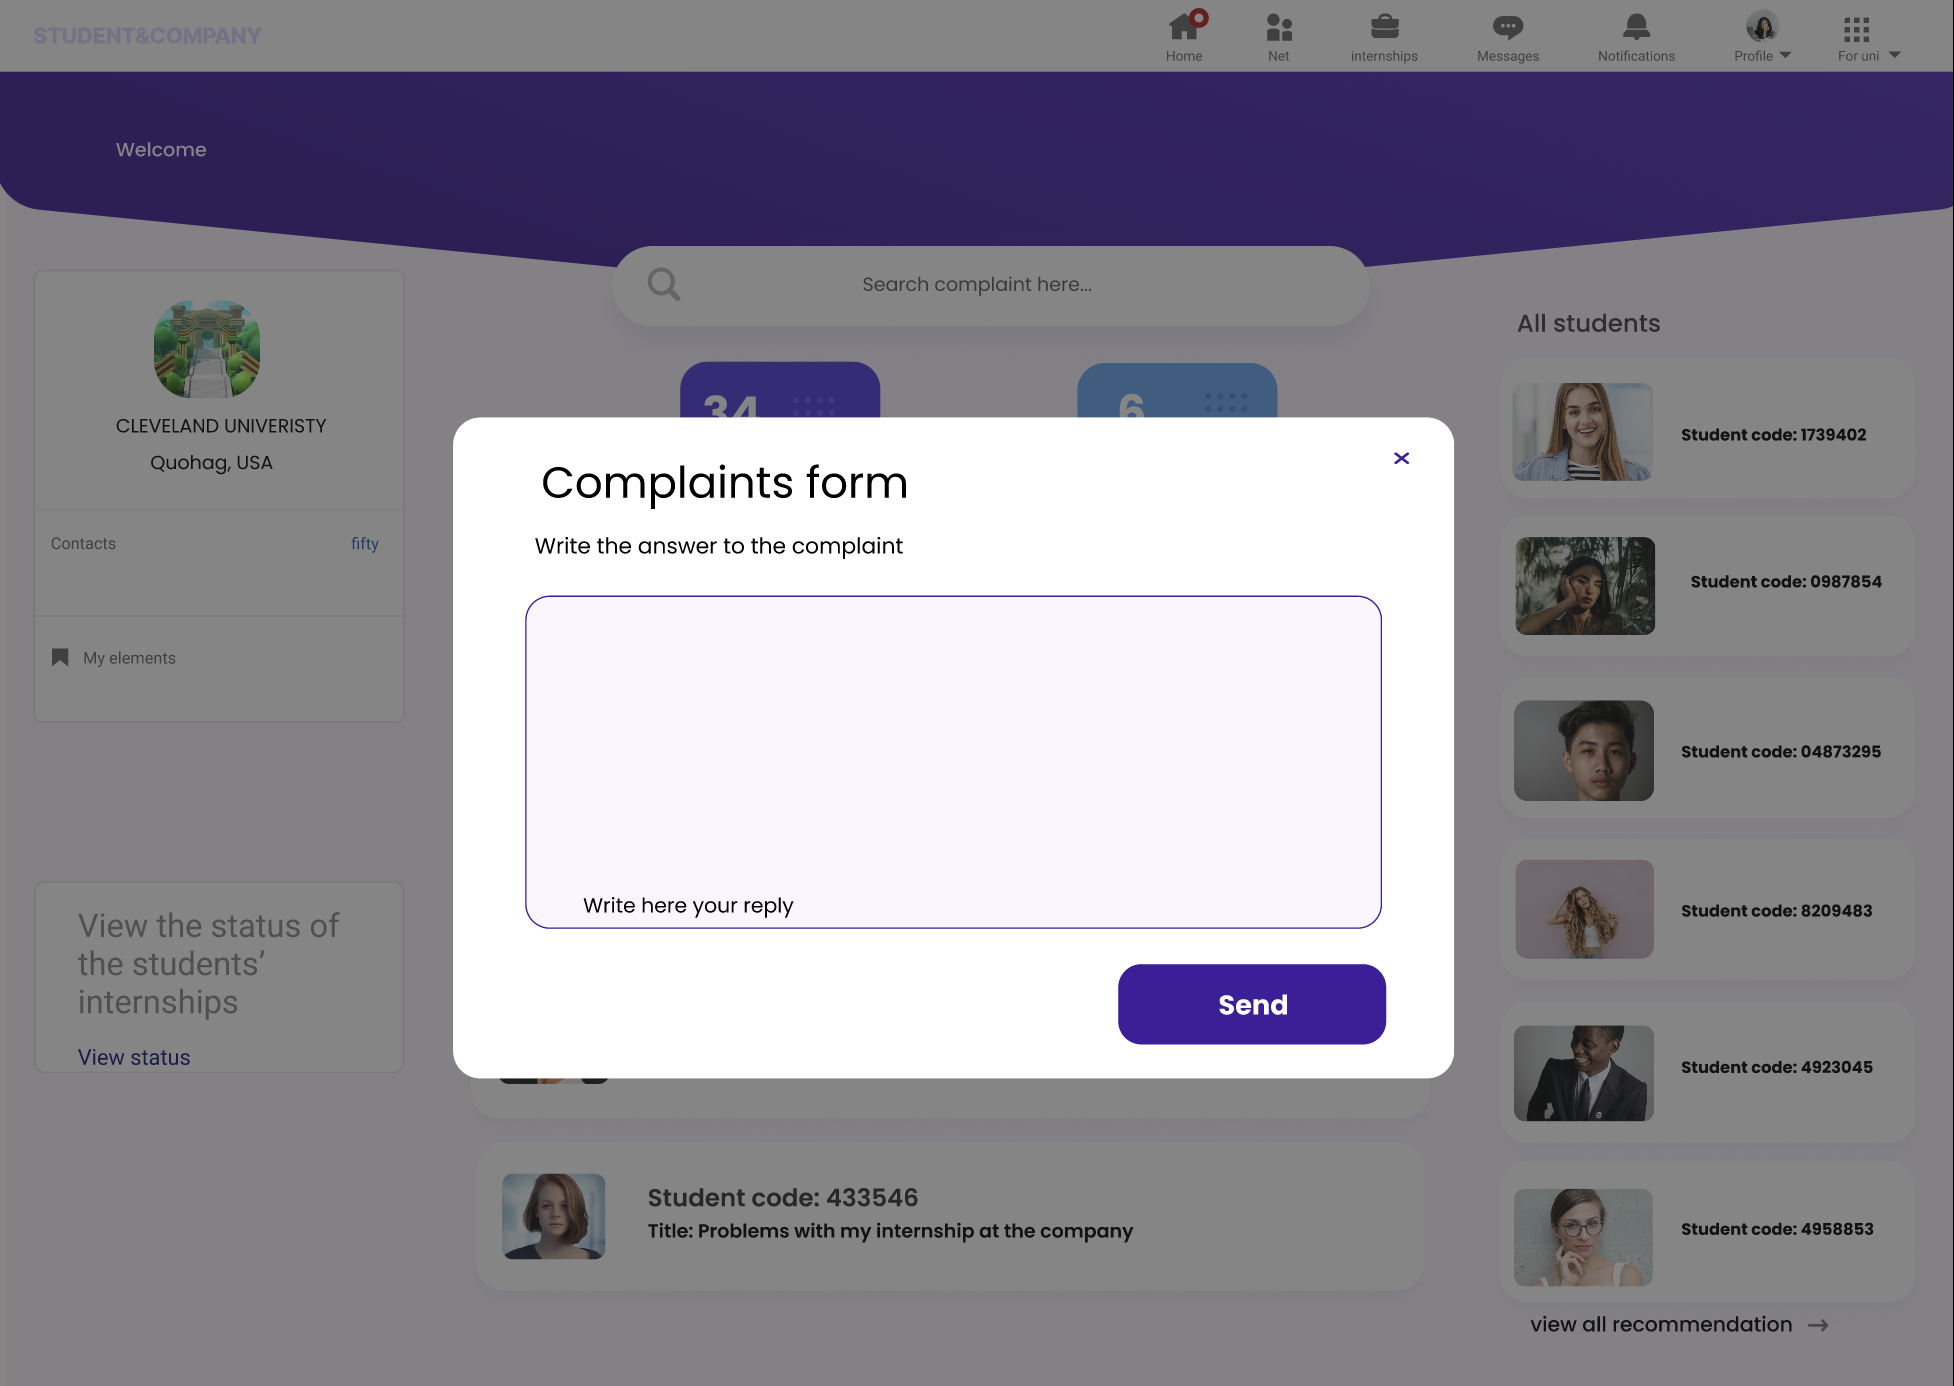
\includegraphics[width=0.5\linewidth]{Images/Interface Images/university interface/Screenshot 2024-12-12 050002.png}
    \caption{Complaints visualization}
    \label{fig:Complaints visualization}
\end{figure}


Complaints are managed through a chat between the university and the involved users, allowing the university to act as an intermediary. This enables the university to assist in resolving the issue or, if necessary, proceed with the conclusion of the internship [Figure \ref{fig: Complaints handling}]

\begin{figure} [H]
    \centering
    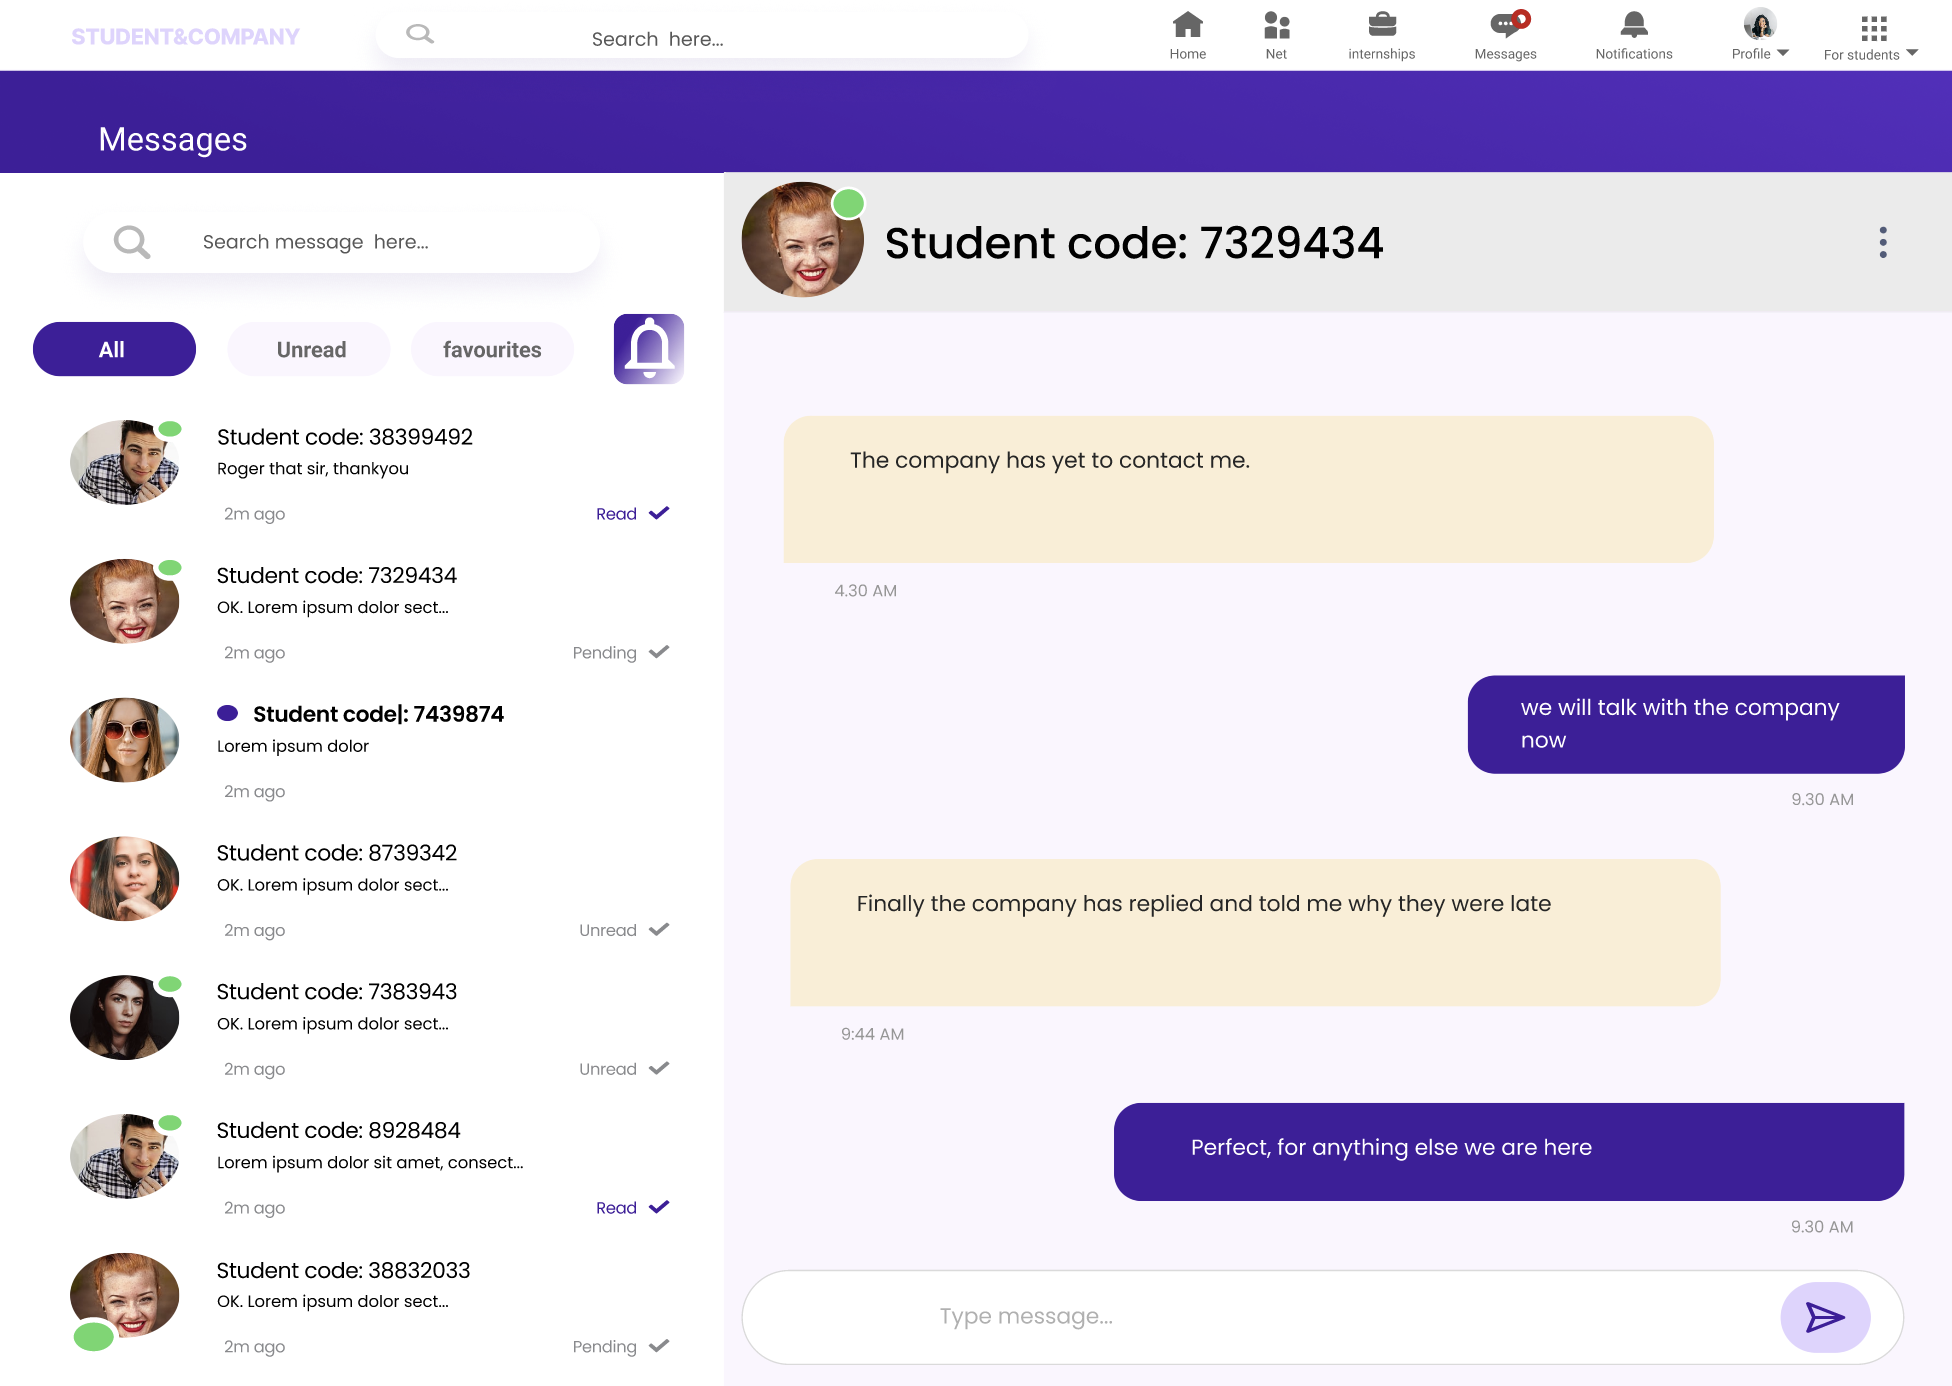
\includegraphics[width=0.5\linewidth]{Images/Interface Images/university interface/Screenshot 2024-12-12 050017.png}
    \caption{Complaints handling}
    \label{fig: Complaints handling}
\end{figure}

\subsection{Common Interfaces}

By clicking on the designated button, users can view all notifications related to important updates, such as changes in internship details, application status, or new internship opportunities that may be of interest to students [Figure \ref{fig:Notifications}].

\begin{figure} [H]
    \centering
    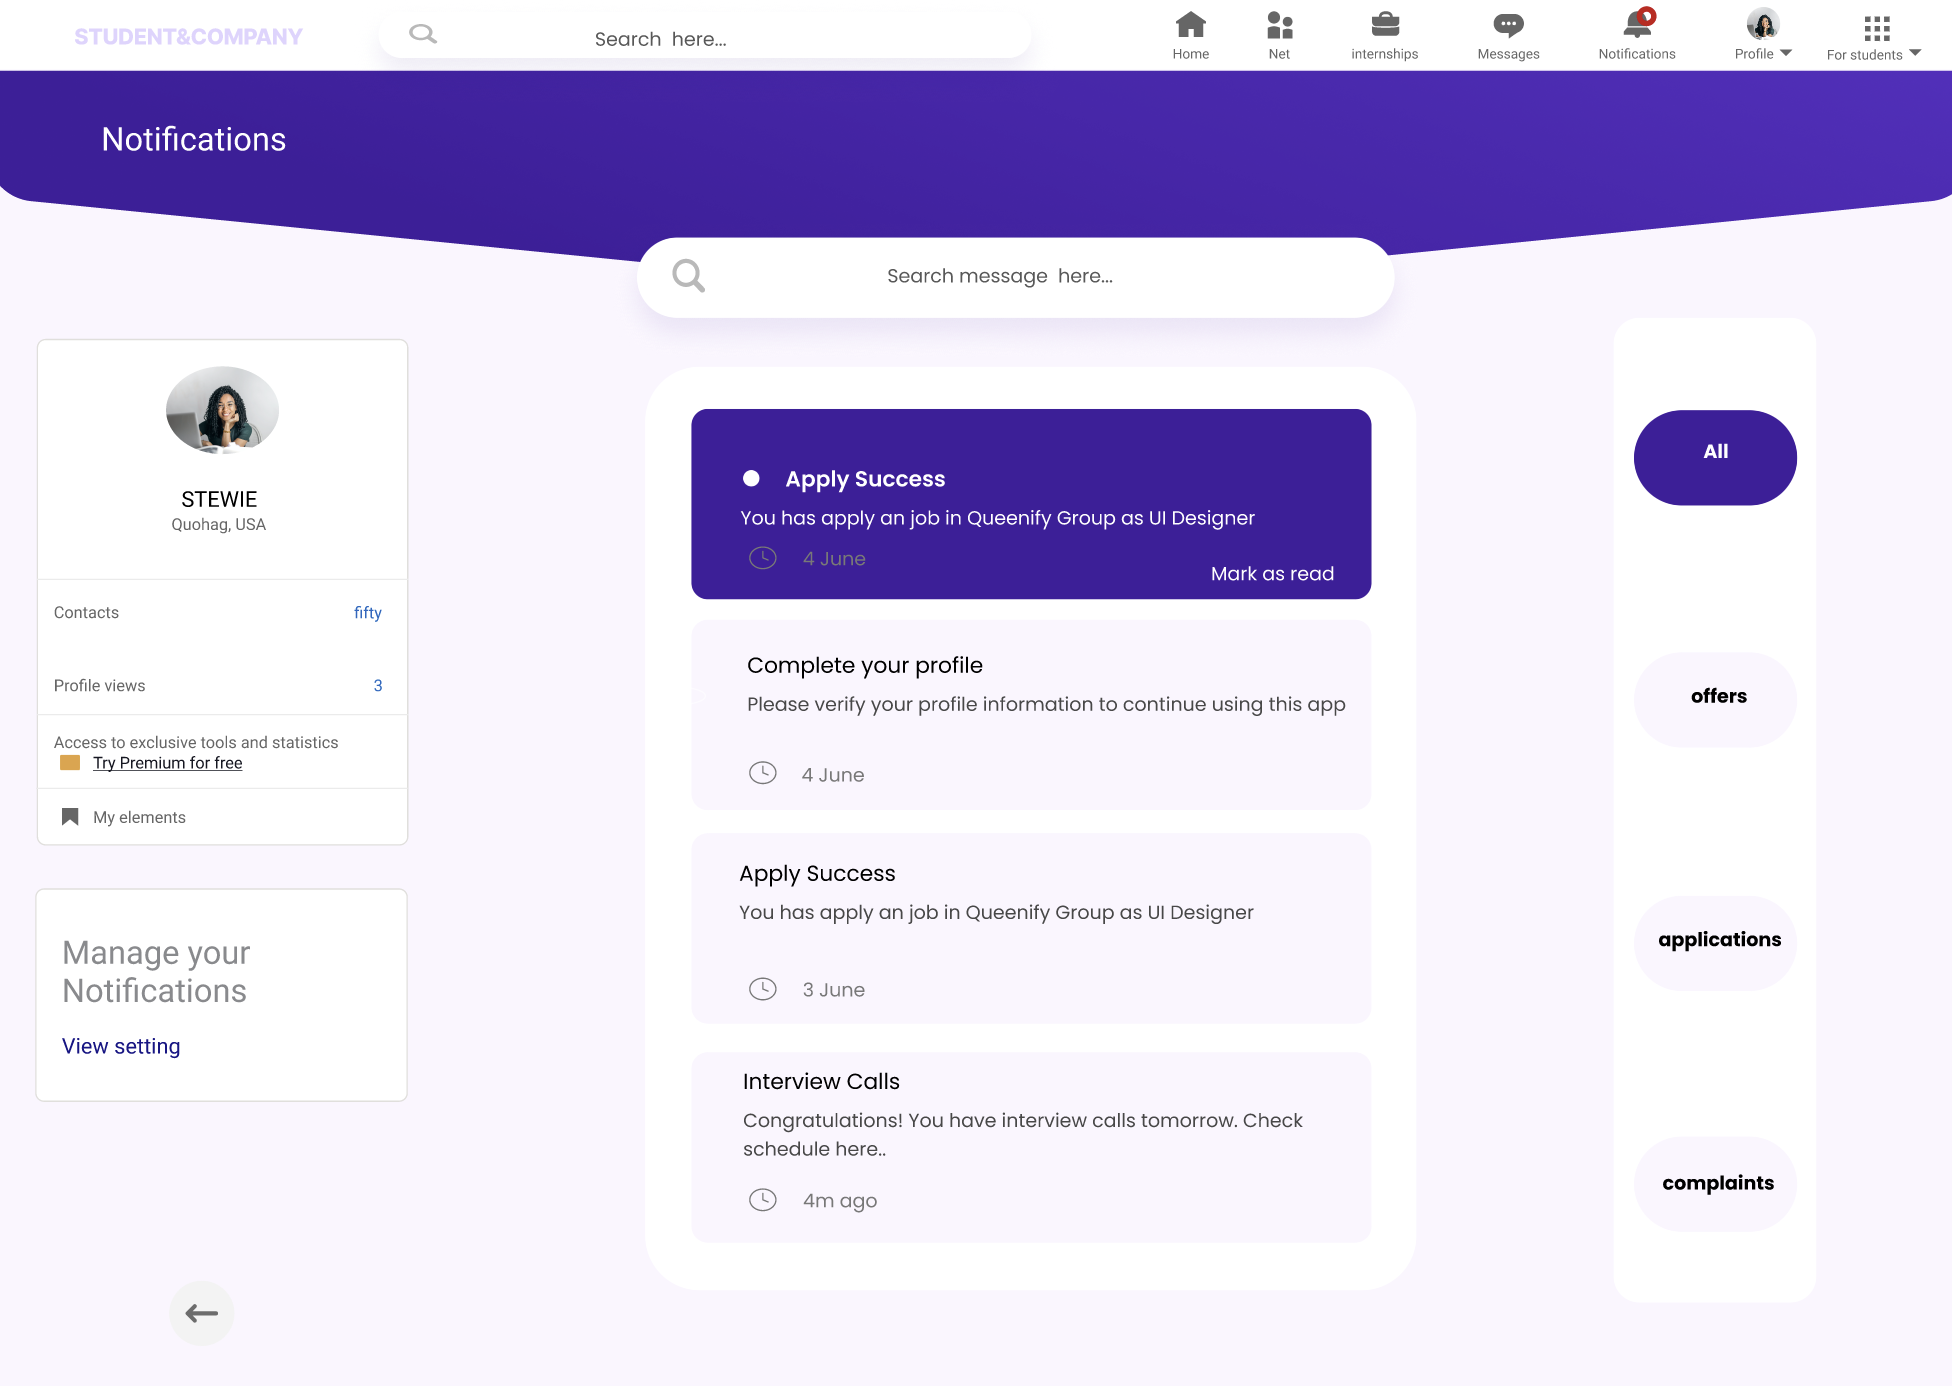
\includegraphics[width=0.5\linewidth]{Images/Interface Images/user interface/Screenshot 2024-12-12 045804.png}
    \caption{Notifications}
    \label{fig:Notifications}
\end{figure}


Users can communicate with each other through a messaging system provided by the platform. Students and companies can interact to discuss internship details, while the university can also use the system to address any complaints or concerns [Figure \ref{fig: Messages}].


\begin{figure} [H]
    \centering
    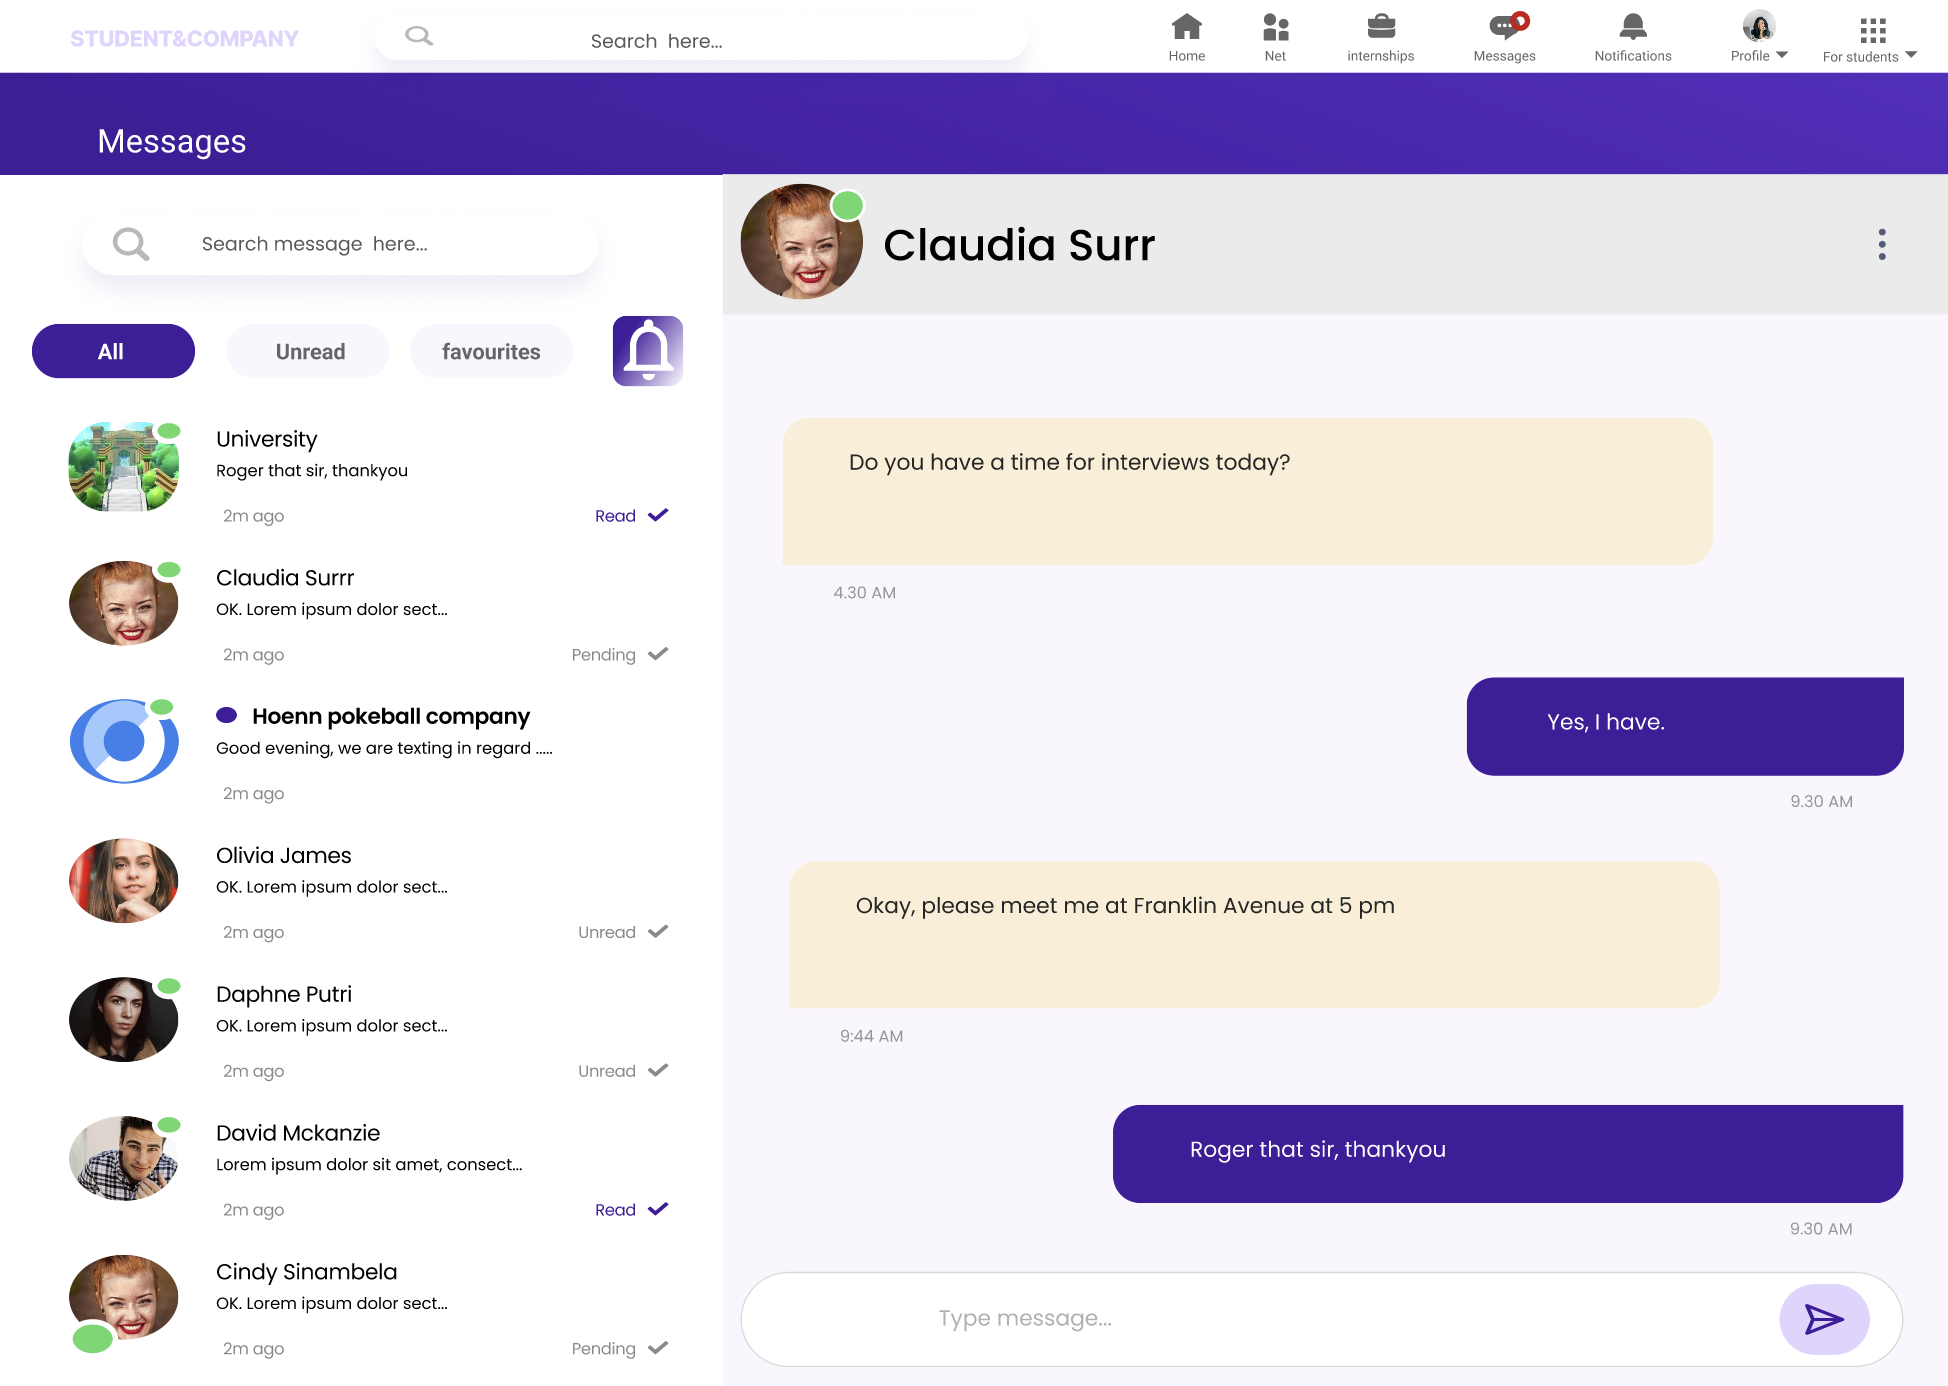
\includegraphics[width=0.5\linewidth]{Images/Interface Images/user interface/Screenshot 2024-12-12 045915.png}
    \caption{Messages}
    \label{fig: Messages}
\end{figure}


Students and companies can also receive feedback requests about their general experience with the platform, provide their own feedback, or submit complaints regarding the progress of the internship once it has started [Figure \ref{fig:Feedback Request}, \ref{fig: Complaints sending}] 

\begin{figure} [H]
    \centering
    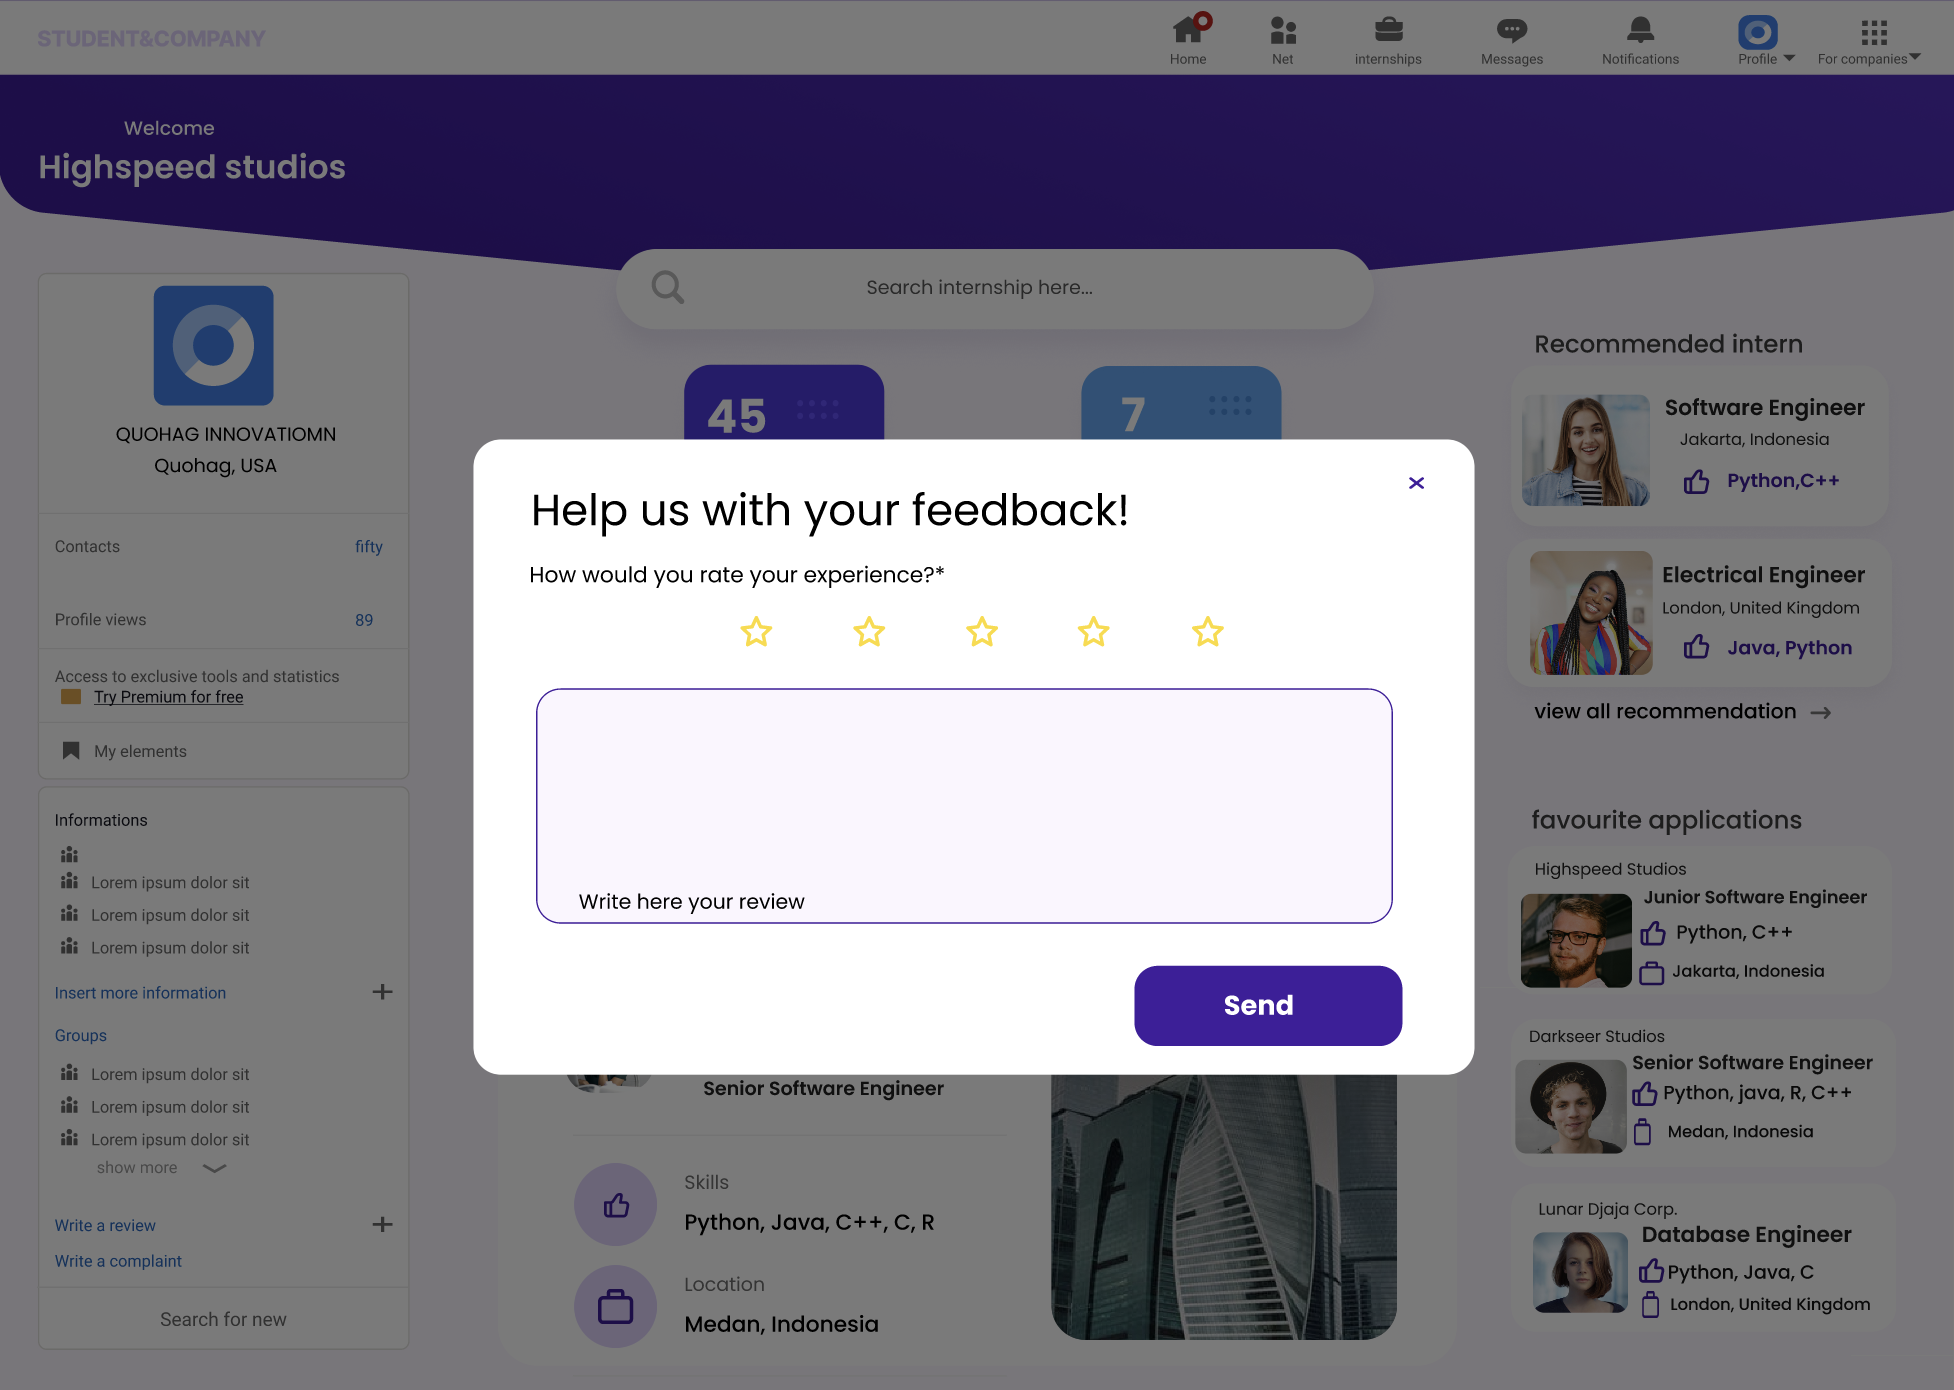
\includegraphics[width=0.5\linewidth]{Images/Interface Images/user interface/Screenshot 2024-12-12 045929.png}
    \caption{Feedback Request}
    \label{fig:Feedback Request}
\end{figure}

\begin{figure} [H]
    \centering
    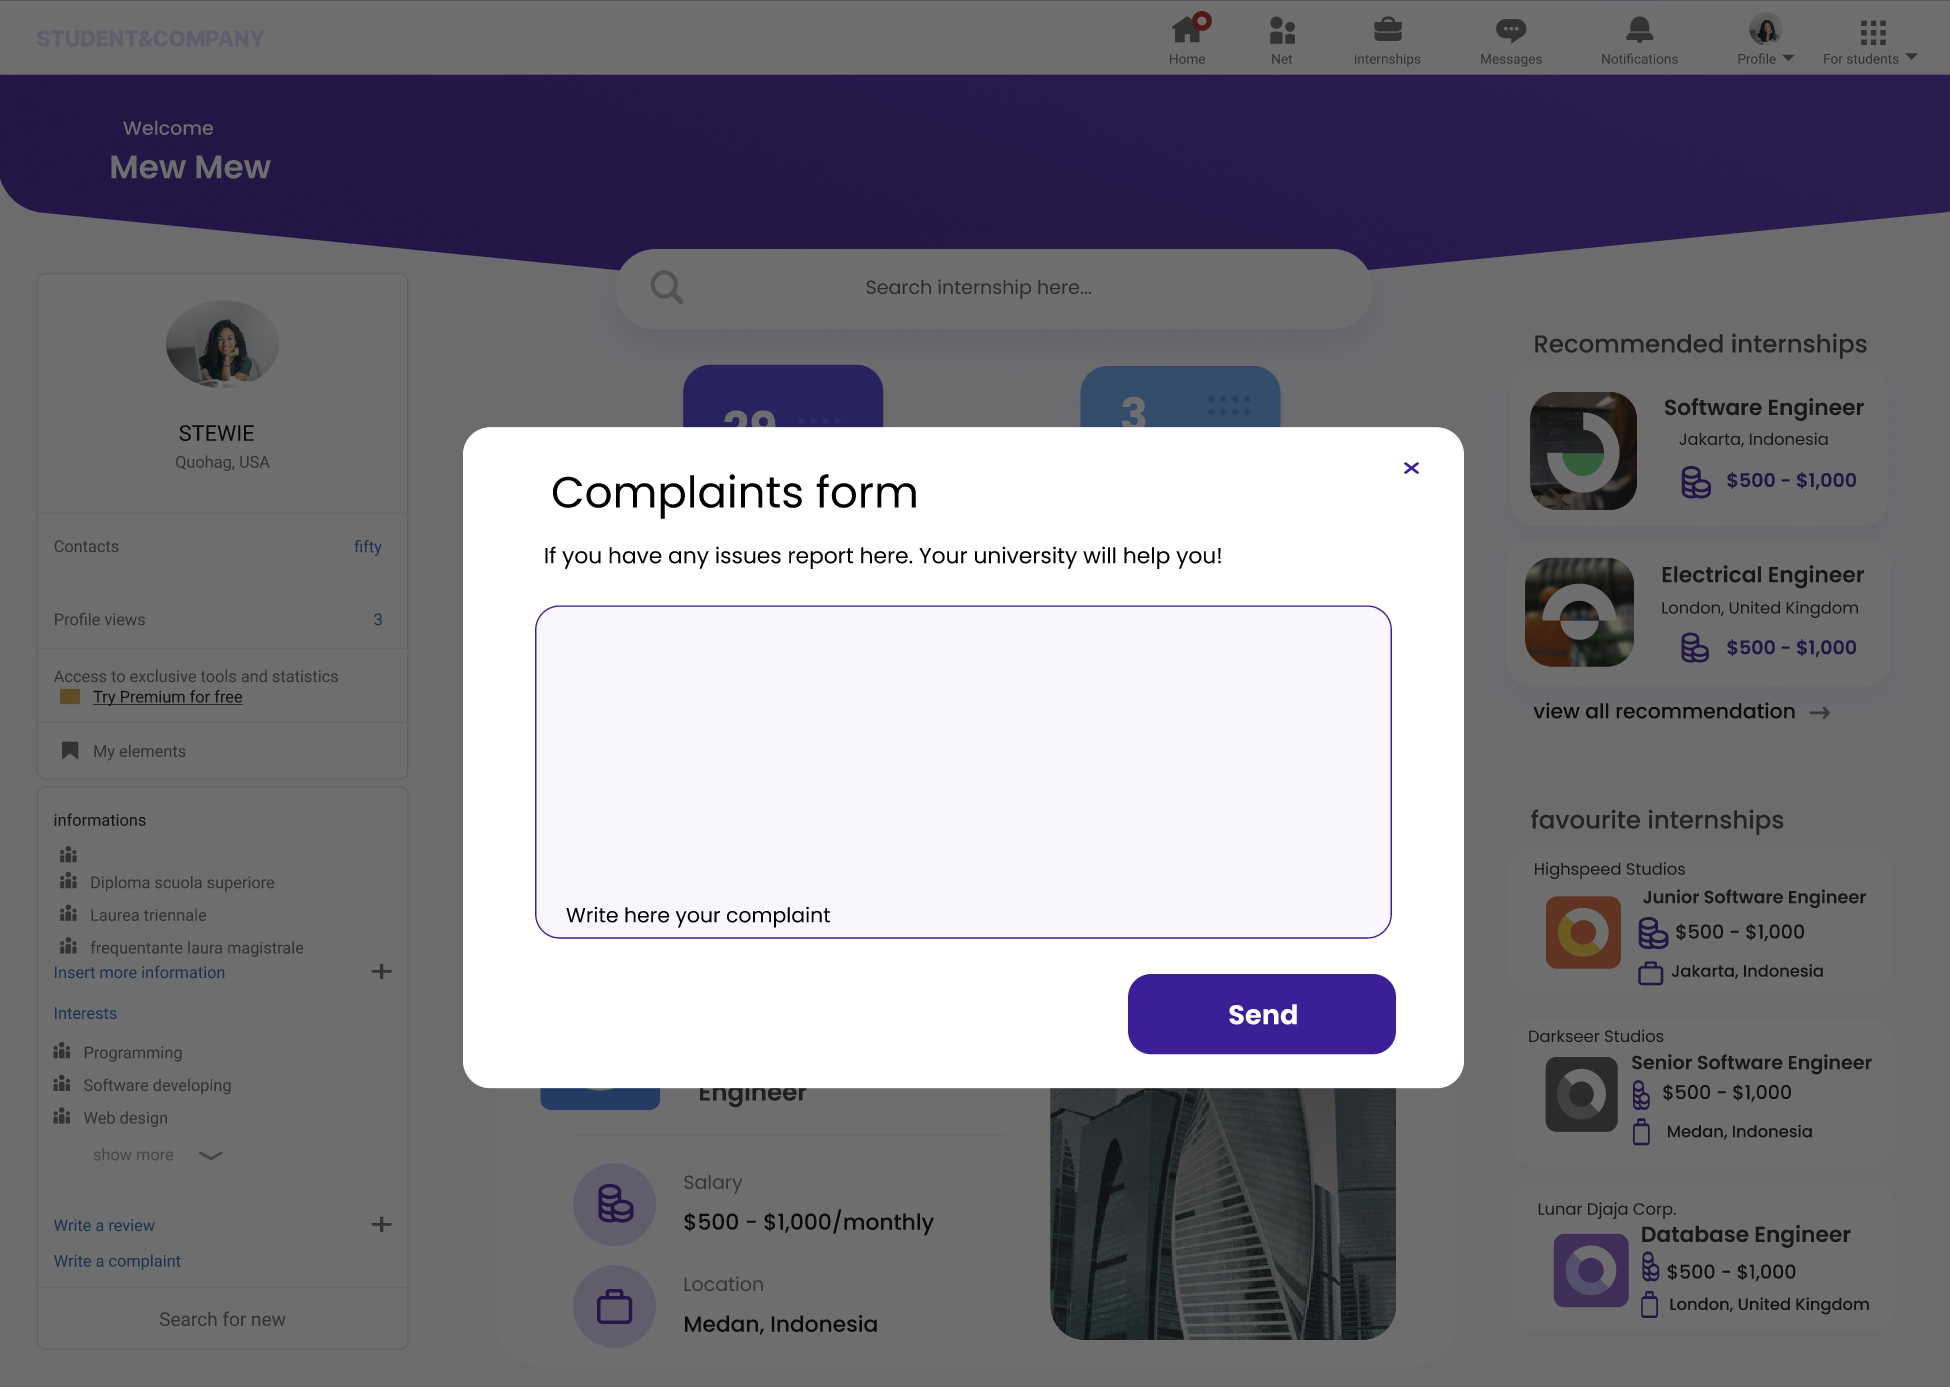
\includegraphics[width=0.5\linewidth]{Images/Interface Images/user interface/Screenshot 2024-12-12 045947.png}
    \caption{Complaints sending}
    \label{fig: Complaints sending}
\end{figure}